\documentclass[oneside]{book}
\usepackage{lmodern}
\usepackage[margin=1in]{geometry}
\usepackage[dvipsnames]{xcolor}
\usepackage[a-3u,pdf17]{pdfx}
\usepackage{hyperref}
\hypersetup{colorlinks=true,linkcolor=Blue}
\usepackage[theorems,breakable]{tcolorbox}
\usepackage[shortlabels]{enumitem}
\usepackage{xfrac}
\usepackage{mathtools}
\usepackage{amssymb}
\usepackage{cleveref}
\usepackage{booktabs}
\usepackage{derivative}
\usepackage{interval}
\intervalconfig{soft open fences,separator symbol={,}}
\usepackage{graphicx}
\graphicspath{{./figures/}}
\usepackage{tikz}
\usetikzlibrary{patterns,positioning,calc}
\usepackage{pgfplots}
\pgfplotsset{samples=100} % possibly uncomment this
\pgfplotsset{compat=1.18}
\usepgfplotslibrary{fillbetween}

\definecolor{myyellow}{RGB}{255,255,168}
\definecolor{mypurple}{RGB}{216,216,255}
\definecolor{mygreen}{RGB}{216,255,216}
\definecolor{myred}{RGB}{255,216,216}
\definecolor{mycyan}{RGB}{204,229,229}

\tcbset{
    common/.style={
            fonttitle=\bfseries,
            coltitle=black,
            boxrule=0pt,
            breakable
        },
    theorem/.style={
            common,
            colback=mypurple,
            colframe=mypurple!95!black,
            fontupper=\itshape{}
        },
}

\newtcbtheorem[number within=section, crefname={definition}{definitions}]
{Definition}{DEFINITION}{
    common,
    colback=myyellow,
    colframe=myyellow!95!black
}{def}

\newtcbtheorem[use counter from=Definition, crefname={remark}{remarks}]
{Remark}{REMARK}{
    common,
    colback=mycyan,
    colframe=mycyan!95!black,
}{remark}

\newtcbtheorem[use counter from=Definition, crefname={theorem}{theorems}]
{Theorem}{THEOREM}{
    theorem
}{thm}

\newtcbtheorem[no counter]
{Proof}{Proof of}{
    common,
    colframe=black!10,
    separator sign={\!\!}
}{pf}

\newtcbtheorem[use counter from=Definition, crefname={example}{examples}]
{Example}{EXAMPLE}{
    common,
    colback=mygreen,
    colframe=mygreen!95!black,
}{ex}

\newtcbtheorem[use counter from=Definition, crefname={corollary}{corollaries}]
{Corollary}{COROLLARY}{
    theorem
}{cor}

\newtcbtheorem[use counter from=Definition, crefname={exercise}{exercises}]
{Exercise}{EXERCISE}{
    common,
    colback=myred,
    colframe=myred!95!black,
}{exercise}

\newtcbtheorem[use counter from=Definition, crefname={proposition}{propositions}]
{Proposition}{PROPOSITION}{
    theorem
}{prop}

\DeclarePairedDelimiterX\Set[1]\{\}{#1}
\DeclarePairedDelimiterX\norm[1]\lVert\rVert{#1}
\DeclarePairedDelimiterX\abs[1]\lvert\rvert{#1}
\DeclarePairedDelimiterXPP{\LN}[1]{\operatorname{\mathrm{ln}}}(){}{#1}
\DeclarePairedDelimiterXPP{\EXP}[1]{\operatorname{\mathrm{exp}}}\{\}{}{#1}

\usepackage{nicematrix}
\newcommand{\R}{\mathbb{R}}
\newcommand{\ER}{\overline{\mathbb{R}}}
\newcommand{\N}{\mathbb{N}}
\newcommand{\Z}{\mathbb{Z}}
\newcommand{\glb}{\mathrm{glb}}
\newcommand{\lub}{\mathrm{lub}}
\newcommand{\LHR}{\stackrel{\text{\tiny L'R}}{=}}
\DeclarePairedDelimiter\sequence{\langle}{\rangle}
\DeclarePairedDelimiterXPP{\bigo}[1]{\mathcal{O}}(){}{#1}

\newcommand{\Dom}{\operatorname{Dom}}
\newcommand{\Cdm}{\operatorname{Cdm}}

\title{%
\LARGE Calculus 2 for Honours Mathematics\\%
\large MATH 138\\%
\normalsize Winter 2019 (1191)}%
\author{Cameron Roopnarine\thanks{\LaTeX{}er}\and Jordan Hamilton\thanks{Instructor}}%
\date{Last updated: \today}

\hypersetup{colorlinks=true,%
linkcolor=Magenta,%
pdftitle={Calculus 2 for Honours Mathematics (MATH 138)},%
pdfauthor={Cameron Roopnarine, Jordan Hamilton},%
pdfsubject={Mathematics},%
pdfkeywords={University of Waterloo, Winter 2019 (1191)}}%

\usepackage{fancyhdr}
\usepackage{lastpage}
\pagestyle{fancy}
\fancyhf{}
\fancyhead[L]{\leftmark}
\fancyhead[R]{\rightmark}
\fancyfoot[L]{Calculus 2 for Honours Mathematics (MATH 138)}
\fancyfoot[C]{}
\fancyfoot[R]{Page \thepage{} of~\pageref*{LastPage}}

\begin{document}

\maketitle
\tableofcontents

\chapter{Characteristics of Time Series}
\section{What is a time series?}
In classical statistics, we normally consider $ X_1,\ldots,X_n\in\mathbf{R}^p $,
a \textbf{simple random sample}.

In particular,
\begin{enumerate}[(1)]
    \item $ X_1,\ldots,X_n $ are i.i.d. (independent and identically distributed)
    \item $ X_i \sim F_\theta $ which is a common distribution characterized
          by $ \theta $.
\end{enumerate}
Examples:
\begin{enumerate}
    \item $ X_i \stackrel{\text{iid}}{\sim} \N{\mu,\sigma^2} $, and we wish to estimate
          and perform inference on $ \mu $ and $ \sigma^2 $.
    \item $ X_i=\begin{bmatrix}
                  Y_i \\
                  Z_i
              \end{bmatrix} $ where $ Y_i $ is a dependent variable, and
          $ Z_i $ is an independent variable.
              {\color{blue}Perhaps we happen to observe
                  $ Y_i $ and $ Z_i $ in pairs, and we stop at a model:}
          \[ Y_i=\beta^\top Z_i+\varepsilon_i\quad \text{where }\varepsilon_i
              \stackrel{\text{iid}}{\sim} \N{0,\sigma_\varepsilon^2} \]
          \begin{Remark}{}{}
              The relationship between $ Y_i $ and $ Z_i $ doesn't
              depend on $ i $, it only depends through the common parameter
              $ \beta $, and it assumes that $ \varepsilon $ has fixed variance
              for each $ i $.
          \end{Remark}
    \item In such settings, one is typically interested in:
          \begin{enumerate}
              \item Prediction: {\color{blue}how based on the data, can we predict
                    how these variables would behave in the future?}
              \item Inference: {\color{blue}how do we use the data to try to estimate
                    and understand better the underlying mechanism which generates
                    the data? For example, a linear model or simple Gaussian model.}
          \end{enumerate}
\end{enumerate}
\begin{Definition}{Time Series}{}
    We say $ X_1,\ldots,X_T $ is an (observed)
    \textbf{time series} of length $ T $ if $ X_t $
    denotes an observation obtained at time $ t $.

    In particular, the observations are ordered in time.
\end{Definition}
\begin{Definition}{Real-valued}{}
    If $ X_t\in\mathbf{R} $, we say $ X_1,\ldots,X_T $ is
    a \textbf{real-valued} or \textbf{scalar} time series.
\end{Definition}
\begin{Definition}{Multivariate}{}
    If $ X_t\in\mathbf{R}^p $, we say $ X_1,\ldots,X_T $
    is a \textbf{multivariate} or \textbf{vector-valued}
    time series.
\end{Definition}

\begin{figure}[!ht]
    \centering
    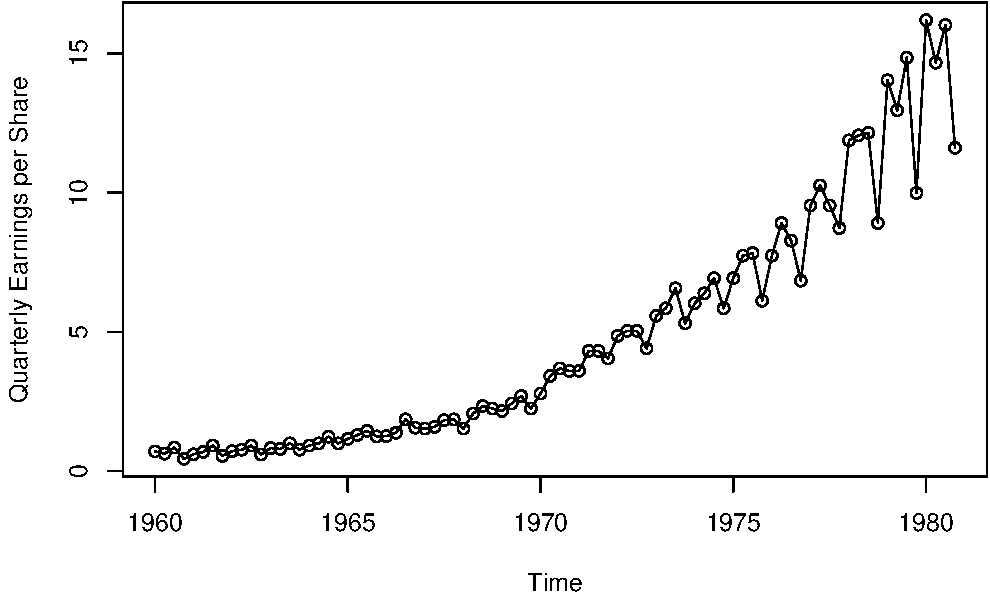
\includegraphics[width=0.75\textwidth]{jj.pdf}
    \caption{Quarterly Johnson and Johnson Earnings}\label{fig:jj}
\end{figure}
Observe that in~\Cref{fig:jj}:
\begin{itemize}
    \item The earnings are steadily increasing over time.
    \item There is heterogeneity in the variance over time.
\end{itemize}

With time series data, we are typically concerned
with the same goals as in classical statistics (prediction and inference).
However, in contrast, with time series, the data often exhibit:
\begin{enumerate}[(1)]
    \item Heterogeneity
          \begin{itemize}
              \item Time trends $ \rightarrow \E{X_t}\neq \E{X_{t+h}} $
              \item Heteroskedasticity
                    $ \rightarrow \Var{X_t}\neq \Var{X_{t+h}} $
          \end{itemize}
          {\color{blue}In classical statistics, it's assumed that all the observations have the
          same distribution which is clearly \underline{not} the case in time series.}
    \item Serial Dependence (Serial Correlation)
          \begin{itemize}
              \item Observations that are temporally close appear to depend
                    on each other.
          \end{itemize}
          {\color{blue}In classical statistics, each successive observation is assumed
          to be independent which is clearly \underline{not} the case in time series.}
\end{enumerate}

\begin{figure}[!ht]
    \centering
    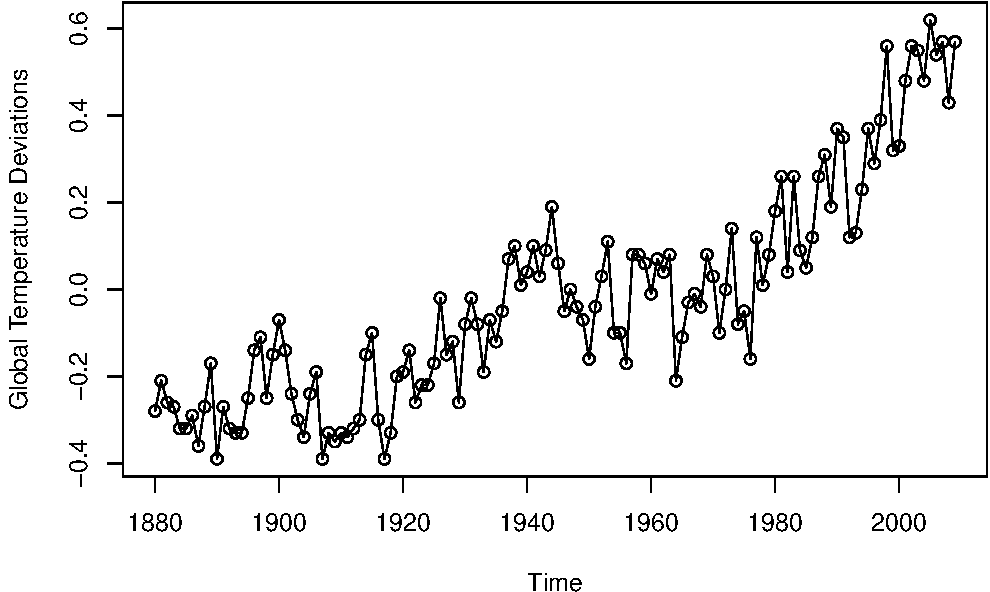
\includegraphics[width=0.75\textwidth]{gtemp.pdf}
    \caption{$ x_t $ is the deviation of global mean
        yearly temperature from the mean computed from 1951--1980}\label{fig:gtemp}
\end{figure}

Observe that in~\Cref{fig:gtemp}:
\begin{itemize}
    \item The global temperature is steadily increasing over time.
    \item There is heterogeneity in the mean over time.
    \item Heterogeneity in the variance over time is not very apparent.
    \item Serial dependence occurs.
\end{itemize}

\begin{Definition}{Time series (Formal Definition)}{}
    We say $ \set{X_t}_{t\in\mathbf{Z}} $
    is a \textbf{time series} if $ \set{X_t : t\in\mathbf{Z}} $
    is a stochastic process indexed by $ \mathbf{Z} $.
\end{Definition}
In other words, there is a common probability space
$ (\Omega,\mathcal{F},\mathbb{P}) $ so that for all
$ X_t:\Omega\to\mathbf{R} $ is a random variable.

In relation to the original definition, we say
$ X_1,\ldots,X_T $ is an \textbf{observed stretch} (\textbf{realization},
\textbf{simple path}) of length $ T $ from $ \set{X_t}_{t\in\mathbf{Z}} $.

    {\color{blue}Formally speaking, we think of a time series as being a little snippet
        of one long sample path the stochastic process for which would characterize
        all the serial dependence, time trends, and heteroskedasticity,
        that exist within a time series.}

\section{Basic Principles of Forecasting}
Consider a time series of length $ T $, namely $ X_1,\ldots,X_T $.
Based on $ X_1,\ldots,X_T $, we would like to produce a ``best guess''
for $ X_{T+h} $:
\[ \hat{X}_{T+h}=\hat{X}_{T+h\mid T}=f_h(X_T,\ldots,X_1) \]
\begin{Definition}{Forecast, Horizon}{}
    For $ h\ge 1 $, our ``best guess''
    \[ \hat{X}_{T+h}=f_h(X_T,\ldots,X_1) \]
    is called a \textbf{forecast} of $ X_{T+h} $
    at \textbf{horizon} $ h $.
\end{Definition}
There are two primary goals in forecasting:
\begin{itemize}
    \item Goal 1: Choose $ f_n $ ``optimally.'' Normally,
          we or the practitioner have some measure, say $ L(\cdot,\cdot) $,
          in mind for determining how ``close'' $ \hat{X}_{T+h} $
          is to the true value, $ X_{T+h} $. We then wish to choose $ f_h $ so that
          $ L(X_{T+h},f_h(X_T,\ldots,X_1)) $
          is minimized.

          \begin{Example}{}{}
              Most common measure $ L(\cdot,\cdot) $ is mean-squared error
              (MSE), where
              \[ L(X,Y)=\E{(X-Y)^2} \]
          \end{Example}
    \item \textbf{Goal 2}: Quantify the uncertainty in the forecast.
          This entails providing some description of how close
          we expect $ \hat{X}_{T+h} $ to be to $ X_{T+h} $.
          \begin{Example}{Why is it important to quantify uncertainty?}{}
              Suppose every minute, we flip a coin and denote
              \begin{itemize}
                  \item $ H\to 1 $
                  \item $ T\to -1 $
                  \item $ X_t= $ outcome in minute $ t $,
                        where $ t=1,\ldots,T $.
              \end{itemize}
              This produces a time series of length $ T $, which is a random
              sequence of $ (1) $'s and $ (-1) $'s. Note $ \E{X_t}=0 $.
              So, if we wish to forecast for $ h\ge 1 $,
              consider $ \hat{X}_{T+h}=f(X_T,\ldots,X_1) $
              \begin{align*}
                  L(X_{T+h},\hat{X}_{T+h})
                   & =\E{(X_{T+h}-\hat{X}_{T+h})^2}                                   \\
                   & =\E{X_{T+h}^2}+\E{\hat{X}_{T+h}^2}-2\E{X_{T+h}\hat{X}_{T+h}}     \\
                   & =\E{X_{T+h}^2}+\E{\hat{X}_{T+h}^2}-2\E{X_{T+h}}\E{\hat{X}_{T+h}} \\
                   & =\E{X_{T+h}^2}+\E{\hat{X}_{T+h}^2}
              \end{align*}
              Furthermore, note that
              $ \E{X_{T+h}^2}=\Var{X_t} $ since $ \E{X_{T+h}}=0 $.

              We can write $ \E{X_{T+h}\hat{X}_{T+h}}=\E{X_{T+h}}\E{\hat{X}_{T+h}} $ since
              $ \hat{X}_{T+h} $ is a function of the data
              $ X_T,\ldots,X_1 $, and hence independent of $ X_{T+h} $.

              We can minimize this by taking $ \hat{X}_{T+h}=0 $. There's
              nothing ``wrong'' with this forecast. But ideally,
              we would also be able to say that the sequence appears to be random,
              and that we don't expect this forecast to be close to the actual value.

                  {\color{blue}Furthermore, for this basic reason, one can always
                      argue that any forecast that's not accompanied with some
                      type of quantification of how close we expect the forecast to be,
                      is at very least hard to interpret; at worst, meaningless
                      because it doesn't
                      describe the accuracy for which we expect the forecast to perform.}
          \end{Example}
\end{itemize}
How can we quantify the uncertainty in forecasting?

Ideal: The predictive distribution:
\[ X_{T+h}\mid X_T,\ldots,X_1 \]
Excellent: Predictive intervals/sets. For some $ \alpha\in(0,1) $
find $ I_\alpha $ so that
\[ \Prob{X_{T+h}\in I_\alpha\given X_T,\ldots,X_1}=\alpha \]
($ \alpha=0.95 $, for example). Often such intervals take the form
\[ I_\alpha=(\hat{X}_{T+h}-\hat{\sigma}_h,\hat{X}_{T+h}+\hat{\sigma}_h) \]
Concluding remarks:
\begin{enumerate}
    \item Estimating predictive distribution leads one towards
          estimating the joint distribution of
          \[ X_{T+h},X_T,\ldots,X_1 \]
          For example, ARMA and ARIMA models.
    \item It is important that we acknowledge that some things cannot be predicted!
\end{enumerate}
``It is tough to make predictions, especially about the future.''---Yogi Berra

\section{Definitions of Stationary}
Given a time series $ X_1,\ldots,X_T $, we are
frequently interested in estimating the joint distribution of
\[ X_{T+h},X_T,\ldots,X_1 \]
which is useful for forecasting and inference.

The joint distribution is a feature of the process
$ \set{X_{t}}_{t\in\mathbf{Z}} $
\[ X_1,\ldots,X_T\xrightarrow[\text{infer}]{}\set{X_t}_{t\in\mathbf{Z}} \]
\begin{itemize}
    \item $ X_1,\ldots,X_T $: Observed data.
    \item $ \set{X_t}_{t\in\mathbf{Z}} $: Stochastic process.
\end{itemize}

Worst case: $ X_t\sim F_t $, where $ F_t $ is a \emph{changing}
function of $ t $. If so, it is hard to pool the data
$ X_1,\ldots,X_T $, to estimate $ F_t $. If
\textbf{serial dependence} occurs; that is, if the
distribution of $ (X_t,X_{t+h}) $
depends strongly on $ t $, then we have a similar problem in estimating
e.g.\ $ \Cov{X_t,X_{t+h}} $.

\begin{Definition}{Strictly stationary}{}
    We say that a time series $ \set{X_t}_{t\in\mathbf{Z}} $
    is \textbf{strictly stationary} (\textbf{strongly stationary})
    if for each $ k\ge 1 $, $ i_1,\ldots,i_k,h\in\mathbf{Z} $,
    \[ (X_{i_1},\ldots,X_{i_k})\stackrel{\text{d}}{=}
        (X_{i_{1}+h},\ldots,X_{i_k+h}) \]
    {\color{blue}If we look at the $ k $-dimensional joint distribution
    $ (X_{i_1},\ldots,X_{i_k}) $
    of the series at points $ i_1,\ldots,i_k $, then
    strict stationary means this is shift-invariant.}
    That is, shifting the window on which
    you view the data, does \underline{not} change its distribution.
    This implies that if $ F_t=\text{CDF} $ of $ X_t $, then
    $ F_t=F_{t+h}=F $
    that is, all variables have a common distribution function.
\end{Definition}
\begin{Definition}{Mean function}{}
    For a time series $ \set{X_t}_{t\in\mathbf{Z}} $, with
    $ \E{X_t^2}<\infty $ for all $ t\in\mathbf{Z} $,
    we denote the \textbf{mean function} of the time series as
    \[ \mu_t=\E{X_t} \]
\end{Definition}
\begin{Definition}{Autocovariance function, Lag}{}
    The \textbf{autocovariance} function of the time series $ \set{X_t}_{t\in\mathbf{Z}} $
    is defined as
    \[ \gamma(t,s)=\E{(X_t-\mu_t)(X_s-\mu_s)}=\Cov{X_t,X_s} \]
\end{Definition}
\begin{Definition}{Weakly stationary, Lag}{}
    We say that a time series $ \set{X_t}_{t\in\mathbf{Z}} $
    is \textbf{weakly stationary} if $ \E{X_t}=\mu $
    (does not depend on $ t $), and if
    \[ \gamma(t,s)=f(\abs{t-s}) \]
    that is, $ \gamma(t,s) $ is a function of $ \abs{t-s} $. In this case,
    we usually write
    \[ \gamma(h)=\Cov{X_t,X_{t+h}} \]
    and we call the input $ h $ the \textbf{lag} parameter.
\end{Definition}
Additional terminology:
\begin{itemize}
    \item The property when $ \E{X_t}=\mu $ does not depend
          on $ t $ is often called the \textbf{first order stationary}.
    \item The property when $ \gamma(t,s)=\gamma(\abs{t-s}) $
          only depends on the lag $ \abs{t-s} $ is called the
          \textbf{second order stationary}.
    \item For a second order stationary process,
          \begin{align*}
              \gamma(h)
               & =\Cov{X_t,X_{t+h}}                                      \\
               & =\Cov{X_{t-h},X_{t-h+h}} & \quad & t\rightarrow{} (t-h) \\
               & =\Cov{X_t,X_{t-h}}                                      \\
               & =\gamma(-h)
          \end{align*}
          Since $ \gamma(h)=\gamma(-h) $, we
          normally, we only record $ \gamma(h) $ for $ h\ge 0 $.
\end{itemize}
\section{White Noise and Stationary Examples}
\begin{Definition}{Strong white noise}{}
    We say $ \set{X_t}_{t\in\mathbf{Z}} $ is a
    \textbf{strong white noise} if $ \E{X_t}=0 $
    and the $ \set{X_t}_{t\in\mathbf{Z}} $ are i.i.d.
\end{Definition}
\begin{Definition}{Weak white noise}{}
    We say $ \set{X_t}_{t\in\mathbf{Z}} $ is a
    \textbf{weak white noise} if $ \E{X_t}=0 $
    and
    \[ \gamma(t,s)=\Cov{X_t,X_s}=\begin{cases}
            \sigma^2 & \abs{t-s}=0 \\
            0        & \abs{t-s}>0
        \end{cases} \]
\end{Definition}
\begin{Definition}{Gaussian white noise}{}
    We say $ \set{X_t}_{t\in\mathbf{Z}} $ is a
    \textbf{Gaussian white noise}
    if $ X_t\stackrel{\text{iid}}{\sim}\N{0,\sigma^2} $.
\end{Definition}
\begin{figure}[!ht]
    \centering
    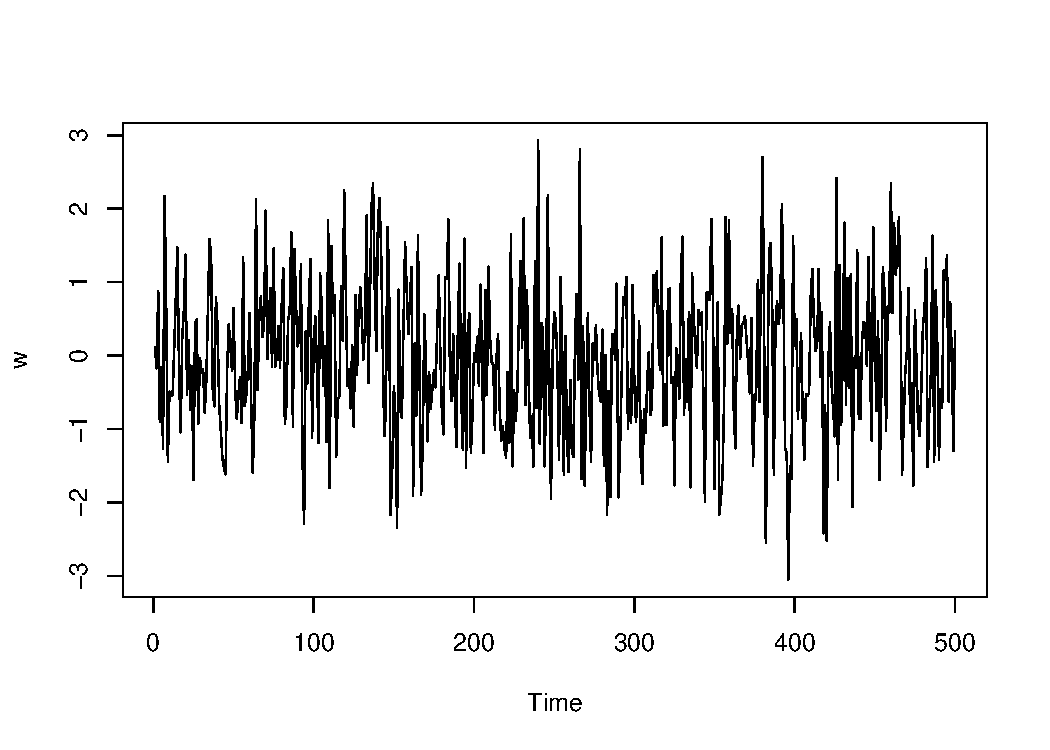
\includegraphics[width=0.75\textwidth]{wn.pdf}
    \caption{Gaussian White Noise of Length 500}\label{fig:wn}
\end{figure}
Figure~\ref{fig:wn} is a Gaussian \emph{white} noise series.
\textbf{White} comes from spectral analysis,
in which a white noise series shares the same spectral properties as white light:
all periodicities occur with equal strength.
\begin{Example}{}{}
    Suppose $ \set{W_t}_{t\in\mathbf{Z}} $
    is a strong white noise, then $ \E{W_t}=0 $;
    that is, it doesn't depend on $ t $.
    \[ \gamma(t,s)=\Cov{W_t,W_s}=\E{W_t W_s}=
        \begin{cases}
            \sigma_W^2 & \abs{t-s}=0 \\
            0          & \abs{t-s}>0
        \end{cases} \]
    only depends on $ \abs{t-s} $.

    $ \set{W_t}_{t\in\mathbf{Z}} $ is
    \textbf{weakly stationary}. Furthermore,
    $ \set{W_t}_{t\in\mathbf{Z}} $ is
    \textbf{strictly stationary}. Let $ k\ge 1 $
    with $ i_1<\cdots i_k $ and $ h\in\mathbf{Z} $, then
    \begin{align*}
        \Prob{W_{i_1}\le t_1,\ldots,W_{i_k}\le t_k}
         & =\prod_{j=1}^k\Prob{W_{i_j}\le t_j}                   & \quad & \text{independence} \\
         & =\prod_{j=1}^k\Prob{W_{{i_j}+h}\le t_j}                                             \\
         & =\Prob{W_{{i_1}+h}\le t_1,\ldots, W_{{i_k}+h}\le t_k}
    \end{align*}
\end{Example}
\begin{Example}{}{}
    Suppose $ \set{W_t}_{t\in\mathbf{Z}} $ is a strong white noise.
    Define $ X_t=W_t+\theta W_{t-1} $ for $ \theta\in\mathbf{R} $.
    Since $ \set{W_t}_{t\in\mathbf{Z}} $ is a strong white noise, we
    have $ \E{W_t}=0 $ for all $ t $, and so we
    have $ \E{X_t}=\E{W_t+\theta W_{t-1}}=\E{W_t}+\theta\E{W_{t-1}}=0 $
    which is first order stationary.
    \[ \gamma(t,s)=\Cov{X_t,X_s}=\begin{cases}
            (1+\theta^2)\sigma_W^2 & \abs{t-s}=0 \\
            \theta\sigma_W^2       & \abs{t-s}=1 \\
            0                      & \abs{t-s}>0
        \end{cases} \]
    We obtain these calculations as follows:
    \begin{itemize}
        \item $ \abs{t-s}=0 $.
              \[ \E{(W_t+\theta W_{t-1})^2}
                  =\E{W_t^2}+\theta^2\E{W_{t-1}^2}+2\E{\theta W_t W_{t-1}}
                  =(1+\theta^2)\sigma_W^2 \]
        \item $ t=s+1 $ (or $ s=t+1 $).
              \[ \E{(W_{s+1}+\theta W_s)(W_s+\theta W_{s-1})}=\theta\E{W_s^2}=\theta\sigma_W^2 \]
              since $ W_{s+1} $ is independent of $ W_s $ and $ W_{s-1} $.
              The calculation is easy to verify.
        \item $ \abs{t-s}>1 $. $ W_t+\theta W_{t-1} $ is independent of
              $ W_s+\theta W_{s-1} $.
    \end{itemize}
    $ \set{X_t}_{t\in\mathbf{Z}} $ is also strictly stationary.
    Suppose $ k\ge 1 $, $ i_1,\ldots,i_k, h\in\mathbf{Z} $
    with $ i_1<\cdots<i_k $, then
    \begin{align*}
        \Prob{X_{i_1}\le t_1,\ldots,X_{i_k}\le t_k}
         & =\Prob{W_{i_1}+\theta W_{{i_1}-1}\le t_1,\ldots,W_{i_k}+\theta W_{{i_k}-1}\le t_k} \\
         & =\Prob*{\begin{bmatrix}
                W_{{i_1}-1} \\
                W_{i_1}     \\
                \vdots      \\
                W_{i_k}
            \end{bmatrix}\in B}                                           \\
         & =\Prob*{\begin{bmatrix}
                W_{{i_1-1}+h} \\
                \vdots        \\
                W_{{i_k}+h}
            \end{bmatrix}\in B}                                           \\
         & =\Prob{X_{{i_1}+h}\le t_1,\ldots,X_{{i_k}+h}\le t_k}
    \end{align*}
    where $ B $ is some subset of $ \mathbf{R}^{i_k-i_1+1} $, and hence
    is shift-invariant.
\end{Example}
\begin{Definition}{Bernoulli shift}{}
    Suppose $ \set{\varepsilon_t}_{t\in\mathbf{Z}} $ is a
    strong white noise. If $ X_t=g(\varepsilon_t,\varepsilon_{t-1},\ldots) $
    for some function $ g:\mathbf{R}^\infty \to \mathbf{R} $, we say that
    $ \set{X_t}_{t\in\mathbf{Z}} $ is a \textbf{Bernoulli shift}.
\end{Definition}
\begin{Theorem}{}{}
    If $ \set{X_t}_{t\in\mathbf{Z}} $ is a Bernoulli shift, then
    $ \set{X_t}_{t\in\mathbf{Z}} $ is strictly stationary.
\end{Theorem}
\begin{Remark}{}{}
    Norbert Wiener conjectured that \textbf{every} stationary
    sequence is a Bernoulli shift, which is not true. The truth is,
    almost every one is.
\end{Remark}
\begin{Exercise}{}{}
    Suppose $ \set{W_t}_{t\in\mathbf{Z}} $ is a strong white noise.
    The \textbf{two-sided random walk} is defined as
    \[ X_t=\sum_{i=0}^{t} W_i+\sum_{i=t}^{-1} W_i  \]
    Show that $ \set{X_t}_{t\in\mathbf{Z}} $ is first order stationary,
    but $ \set{X_t}_{t\in\mathbf{Z}} $ is \underline{not} second order stationary.
\end{Exercise}
\section{Weak versus Strong Stationary}
Sadly, $ \set{X_t}_{t\in\mathbf{Z}} $ is strictly stationary does \underline{not} imply
$ \set{X_t}_{t\in\mathbf{Z}} $ is weakly stationary.
\begin{Example}{}{}
    Suppose $ X_t\stackrel{\text{iid}}{\sim} $ Cauchy Random Variables;
    that is,
    \[ \Prob{X_t\le s}=\int_{-\infty}^{s} \frac{1}{\pi(1+x^2)}\, d{x}  \]
    Then, $ \E{X_t} $ does not exist, and hence $ \set{X_t}_{t\in\mathbf{Z}} $ cannot
    be weakly stationary. However, $ \set{X_t}_{t\in\mathbf{Z}} $ is strictly
    stationary in this case since $ \set{X_t}_{t\in\mathbf{Z}} $ is a strong
    white noise.
\end{Example}
\begin{Theorem}{}{strongly_imp_weakly}
    If $ \set{X_t}_{t\in\mathbf{Z}} $ is strongly stationary and $ \E{X_0^2}<\infty $,
    then $ \set{X_t}_{t\in\mathbf{Z}} $ is weakly stationary.
\end{Theorem}
\begin{Proof}{\Cref{thm:strongly_imp_weakly}}{}
    Note that if $ \set{X_t}_{t\in\mathbf{Z}} $ is strictly stationary,
    \[ (X_t)\stackrel{\text{d}}{=}(X_0) \]
    so that $ \E{X_t}=\E{X_0} $ which does not depend on $ t $, and also
    \[ \Var{X_t}=\Var{X_0} \]
    By the Cauchy-Schwarz inequality,
    \[ \gamma(t,s)=\Cov{X_t,X_s}\le \Var{X_t}<\infty \]
    and suppose $ t<s $,
    \[ \Cov{X_t,X_s}=\Cov{X_0,X_{s-t}}=f(\abs{s-t}) \]
    since it is shift-invariant, and hence if we shift everything over by $ t $,
    \[ (X_t,X_s)\stackrel{\text{d}}{=}(X_{t-t},X_{s-t})\stackrel{\text{d}}{=}(X_0,X_{s-t}) \]
\end{Proof}
\begin{Definition}{Gaussian process}{}
    $ \set{X_t}_{t\in\mathbf{Z}} $ is said to be a
    \textbf{Gaussian process} (\textbf{Gaussian time series}) if
    for each $ k\ge 1 $, $ i_1<i_2<\cdots<i_k $ we have
    \[ (X_{i_1},\ldots,X_{i_k})\sim
        \Mvn{\symbf{\mu}_k(i_1,\ldots,i_k),\symbf{\Sigma}_{k\times k}(i_1,\ldots,i_k)} \]
    \[ \symbf{\mu}_k=\begin{bmatrix}
            \E{X_{i_1}} \\
            \vdots      \\
            \E{X_{i_k}}
        \end{bmatrix}\quad
        \symbf{\Sigma}_{k\times k}=
        \Cov{X_{i_j},X_{i_r}}_{1\le j,\, r\le k} \]
\end{Definition}
\begin{Theorem}{}{weak_gaussian_imp_strictly}
    If $ \set{X_t}_{t\in\mathbf{Z}} $ is weakly stationary and a Gaussian process, then
    $ \set{X_t}_{t\in\mathbf{Z}} $ is strictly stationary.
\end{Theorem}
\begin{Proof}{\Cref{thm:weak_gaussian_imp_strictly}}{}
    If $ \set{X_t}_{t\in\mathbf{Z}} $ is weakly stationary, then $ \E{X_t}=\mu $ for all $ t $.
    \[ (X_{i_1},\ldots,X_{i_k})\rightarrow
        \begin{bmatrix}
            \E{X_{i_1}} \\
            \vdots      \\
            \E{X_{i_k}}
        \end{bmatrix}=\begin{bmatrix}
            \mu    \\
            \vdots \\
            \mu
        \end{bmatrix}=\symbf{\mu}=
        \begin{bmatrix}
            \E{X_{{i_1}+h}} \\
            \vdots          \\
            \E{X_{{i_k}+h}}
        \end{bmatrix} \]
    Also,
    \begin{align*}
        \Var{X_{i_1},\ldots,X_{i_k}}
         & =\Cov{X_{i_j},X_{i_r}}_{1\le j,\, r\le k} \\
         & =\Cov{X_0,X_{i_r-i_j}}_{1\le j,\, r\le k} \\
         & =\Cov{X_0,X_{i_r+h},X_{i_r+h-(i_j+h)}}    \\
         & =\Cov{X_{i_j+h},X_{i_r+h}}                \\
         & =\Var{X_{i_1+h},\ldots,X_{i_k+h}}
    \end{align*}
\end{Proof}
\begin{Example}{}{}
    Using the Gaussian assumption
    \[ (X_{i_1},\ldots,X_{i_k})
        \stackrel{\text{d}}{=}\Mvn{\symbf{\mu},\symbf{\Sigma}_{k\times k}}
        \stackrel{\text{d}}{=}(X_{i_1+h},\ldots,X_{i_k+h}) \]
    Hence $ \set{X_{t}}_{t\in\mathbf{Z}} $ is strictly stationary
    in this case.
\end{Example}
\begin{Exercise}{}{}
    Prove that if $ \set{X_t}_{t\in\mathbf{Z}} $ is \underline{not}
    weakly stationary; that is, either $ \E{X_t} $ depends on $ t $
    or $ \gamma(t,s) $ does not depend on the lag,
    then $ \set{X_t}_{t\in\mathbf{Z}} $ is \underline{not} strictly stationary.
\end{Exercise}

\section{\texorpdfstring{$ \dagger $}{†} Theoretical L2 Framework for Time Series}
\begin{itemize}
    \item $ X_t = \lim\limits_{{h} \to {\infty}} X_{h,t} $. In what sense
          does this limit exist?
    \item How ``close'' are two random variables $ X $ and $ Y $?
    \item Is there a random variable that achieves
          \[ \inf_{y\in S}d(Y,S) \]
\end{itemize}
\begin{Definition}{$ L^2 $ space}{}
    Consider a probability space $ (\Omega,\mathcal{F},\mathbb{P}) $.
    The space $ L^2 $ is the set of random variables
    $ X:\Omega\to\mathbf{R} $ measurable so that $ \E{X^2}<\infty $.
\end{Definition}
\begin{Definition}{$ L^2 $-time series}{}
    We say that $ \set{X_t}_{t\in\mathbf{Z}} $ is
    and $ L^2 $-time series if $ X_t\in L^2 $ for all
    $ t\in\mathbf{Z} $.
\end{Definition}
$ L^2 $ is a Hilbert space when equipped
with inner product, $ X,Y\in L^2 $.
\[ \innerp{X}{Y}=\E{XY} \]
$ \innerp{}{} $ is an inner product since it is
\begin{enumerate}[(1)]
    \item Linear: $ \innerp{aX+bY}{Z}=a\innerp{X}{Z}+b\innerp{Y}{Z} $.
    \item ``Almost'' Positive Definite:
          $ \innerp{X}{X}=\E{X^2}=0 \iff X=0 $ almost surely.
          Which implies $ \Prob{X=0}=1 $.
    \item Symmetric: $ \innerp{X}{Y}=\innerp{Y}{X} $.
\end{enumerate}
$ L^2 $ is complete with this inner product; that is,
whenever $ X_n\in L^2 $ so that $ \E{(X_n-X_m)^2}\to 0 $
as $ n,m\to\infty $, then there exists $ X\in L^2 $
so that $ X_n\to X $; that is, $ \E{(X_n-X)^2}\to 0 $.
This follows from the ``famous'' Riesz-Fischer Theorem.
\subsection{Useful Tools for Time Series}
\begin{enumerate}[(1)]
    \item \textbf{Existence of Limits}
          \[ X_{t,n}=\sum_{j=0}^{n} \Psi_j \varepsilon_{t-j}
          \]
          $ \set{\varepsilon_t}_{t\in\mathbf{Z}} $ is a strong white noise.
          Since for $ n>m $,
          \[ \E{(X_{t,n}-X_{t,m})^2}
              =\E[\bigg]{\biggl(\sum_{j=m+1}^{n} \Psi_j \varepsilon_{t-j}\biggr)^{\!2}}
              =\sum_{j=m+1}^{n} \Psi_j^2\sigma_{\varepsilon}^2\to 0\text{ as }
              n,m\to \infty \]
          only if $ \sum_{j=0}^{\infty} \Psi_j^2<\infty $, then there \textbf{must}
          exist a random variable $ X_t $ (by the completeness of $ L^2 $), so that
          \[ X_t=\lim\limits_{{n} \to {\infty}} X_{t,n}=\sum_{j=0}^{\infty}
              \Psi_j \varepsilon_{t-j} \]
    \item \textbf{Projection Theorem and Forecasting}.
          Forecasting can be often cast as finding a random variable $ Y $ among
          a collection of possible forecasts $ \mathcal{M} $ (e.g.
          $ \mathcal{M}=\Span{X_T,\ldots,X_1} $) so that
          \[ Y={\arg\inf}_{Z\in\mathcal{M}}\E{(X_{T+h}-Z)^2} \]
          When $ \mathcal{M} $ is a closed linear subspace of $ L^2 $,
          the Projection Theorem guarantees that such a $ Y $ exists,
          and it must satisfy
          \[ \innerp{X_{T+h}-Y}{Z}=0\quad\forall Z\in\mathcal{M} \]
          must be in the orthogonal complement.
\end{enumerate}

\section{Signal and Noise Models}
``Ideally,'' a time series that we are considering
was generated from a stationary process. If so,
we can pool data to estimate the processes underlying structure
(e.g.\ its marginal distribution and serial dependence structure)

Most time series are evidently \underline{not} stationary.

Looking back at Figure~\ref{fig:jj}:
\begin{itemize}
    \item Mean appears to increase, so it is not first order stationary;
    \item Variability also appears to increase, so it is not
          second order stationary;
    \item Therefore, it is not strictly stationary.
\end{itemize}
Signal and Noise Model: $ X_t=S_t+\varepsilon_t $
\begin{itemize}
    \item $ S_t $ is the \textbf{deterministic}
          ``signal'' or ``trend'' of the series
    \item $ \varepsilon_t $ is the ``noise'' added
          to the signal satisfying $ \E{\varepsilon_t}=0 $, hence
          $ \E{X_t}=\E{S_t+\varepsilon_t}=\E{S_t} $.
          There exists a (strong) white noise $ \set{W_t}_{t\in\mathbf{Z}} $
          so that
          \[ \varepsilon_t=g(W_t,W_{t-1}\ldots,)\quad\text{[Stationary Noise]} \]
          \[ \varepsilon_t=g_t(W_t,W_{t-1}\ldots,)\quad\text{[Non-stationary Noise]} \]
          The terms $ \set{W_t}_{t\in\mathbf{Z}} $ are often called the
          ``innovations'' or ``shocks'' during the random behaviour
          of $ X_t $.

              {\color{blue}$ g $ is used to try to capture noise that can
                  potentially have serial dependence.}
\end{itemize}
\begin{Example}{}{}
    An example of a function $ g $ so that $ \varepsilon_t=g_t(W_t,W_{t-1},\ldots) $
    might be a \textbf{random walk}; that is, $ \varepsilon_t=\sum_{j=0}^{t} W_j $.
    Another example could be the \textbf{changing variance models}; that is,
    $ \varepsilon_t=\sigma(t)W_t $.
\end{Example}
Our goal is to estimate $ S_t $, and then infer the structure of $ \varepsilon_t $.

In Figure~\ref{fig:gtemp}, the model appears to be non-stationary
(trending upwards over time),
so we might try the signal and noise model. We might posit
a linear trend, or even higher order functions.

For the temperature data, we may posit that
\[ S_t=\beta_0+\beta_1 t\quad\text{[Linear Trend]} \]
The trend may be estimated by ordinary least squares (OLS).
We choose $ \beta_0 $ and $ \beta_1 $ to minimize
\[ \sum_{t=1}^{T} \bigl[X_t-(\beta_0+\beta_1 t)\bigr]^2 \]
This can be done in R using the \code{lm()} command, and
can easily be computed with calculus. Figure~\ref{fig:gtemp_lm}
is a small example of the global temperature data superimposed
with \code{lm()}'s estimate.
\begin{figure}[!ht]
    \centering
    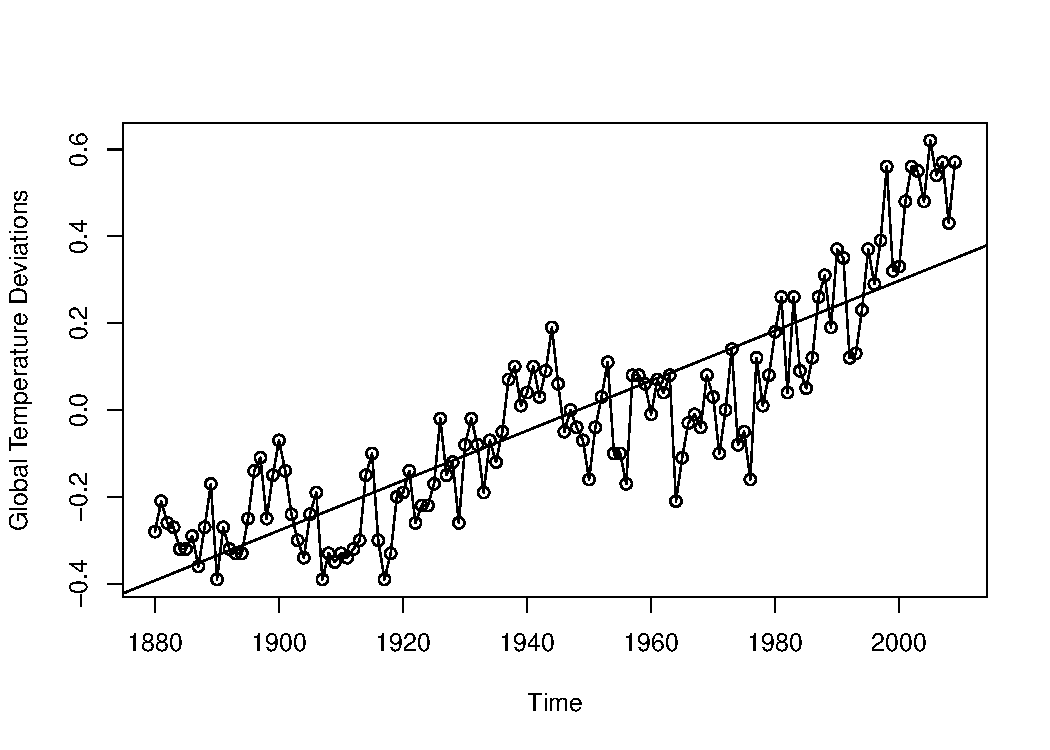
\includegraphics[width=0.75\textwidth]{gtemp_lm.pdf}
    \caption{OLS estimate of a linear trend.}\label{fig:gtemp_lm}
\end{figure}
Let's introduce some terminology about trends.
\begin{Definition}{Detrended time series}{}
    Detrending a time series constitutes computing the
    residuals based on an estimate for the signal/trend.

    A \textbf{detrended time series} is a time series of such residuals.
    \begin{enumerate}
        \item Estimate $ S_t\to \hat{S_t} $
        \item Detrend series: $ X_t-\hat{S_t}=Y_t $
              where $ Y_t $ is the ``detrended'' series.
    \end{enumerate}
\end{Definition}

If the trend is zero, there appears to be a substantial serial
dependence remaining in the time series.

\section{Time Series Differencing}
Signal and Noise Model: $ X_t=S_t+\varepsilon_t $. Hopefully,
upon estimating $ S_t $ with $ \hat{S}_t $,
we find $ X_t-\hat{S}_t=\hat{\varepsilon}_t $ (detrended series)
looks reasonably stationary. If the residuals would be
reasonably stationary, we might
proceed in estimating their underlying structure of $ \set{\hat{\varepsilon}_t}_{t=1,\ldots,T} $.
as if it were stationary. {\color{blue}In particular, we might try to estimate their marginal
        distributions and/or their serial dependence structure. If we thought those estimates
        were reasonably good, we would have a good idea of how the time series $ X_t $ behaves.}

\textbf{Random Walk with Drift Model}. Let $ \varepsilon_t $ be a strong white noise.
\begin{align*}
    X_t
     & =\delta+X_{t-1}+\varepsilon_t                                                                                  \\
     & =\delta+\delta+X_{t-2}+\varepsilon_{t-1}+\varepsilon_t                                                         \\
     & =\delta+\delta+\delta+X_{t-3}+\varepsilon_{t-2}+\varepsilon_{t-1}+\varepsilon_{t}                              \\
     & \vdots                                                                            & \quad & \text{$ t $ times} \\
     & =t\delta+X_0+\sum_{j=1}^{t} \varepsilon_j
\end{align*}
where we note that $ t\delta+X_0=S_t $ is a linear signal,
and $ \sum_{j=1}^{t} \varepsilon_j $ is a
random walk noise.

Notice that under the Random Walk Model.
\[ X_t-X_{t-1}=\nabla X_t=\delta+\varepsilon_t \]
So, if $ X_t $ follows a random walk model, the series $ Y_t=\delta X_t $
should behave like a white noise shifted by $ \delta $.

\begin{Definition}{Differenced time series}{}
    Differencing a time series constitutes
    computing the difference between successive terms.

    A \textbf{differenced time series} is a time series of such differences.
    The first differenced series is denoted
    \[ \nabla X_t=X_t-X_{t-1} \]
    and is the series of length $ T-1 $, namely
    \[ X_2-X_1,X_3-X_2,\ldots,X_T-X_{T-1} \]
    Higher order differences are calculated recursively, so
    \[ \nabla^d X_t=\nabla^{d-1}\nabla X_t \]
    where $ \nabla^d $ is the $ d^{\text{th}} $ order difference and
    we define $ \nabla^0 X_t=X_t $.
\end{Definition}

Detrending and Differencing are both ways of reducing a
(potentially non-stationary) time series
to an approximately stationary series.

\underline{Differencing vs. Detrending}

\emph{Pros}:
\begin{itemize}
    \item Differencing does not require the parameter estimation
          (don't need to estimate $ S_t $).
    \item Higher order differencing can reduce even very
          ``trendy'' series to look more like noise.
\end{itemize}
\emph{Cons}:
\begin{itemize}
    \item Differencing can ``wash away'' features of the series,
          and introduce more complicated structures.
    \item The trend is often of interest, and good estimates
          of the trend lead to improved long-range forecasts.
\end{itemize}
\begin{Example}{Differencing can complicate time series}{}
    $ X_t=W_t $ where $ W_t $ is a strong white noise.
    \[ \nabla X_t=W_t-W_{t-1}=Y_t \]
    \[ \gamma_X(h)=\Cov{X_t,X_{t+h}}=\begin{cases}
            \sigma_W^2 & h=0    \\
            0          & h\ge 1
        \end{cases} \]
    More complicated:
    \[ \gamma_Y(h)=\Cov{Y_t,Y_{t+h}}=\begin{cases}
            2\sigma_W^2 & h=0    \\
            -\sigma_W^2 & h=1    \\
            0           & h\ge 2
        \end{cases} \]
\end{Example}

\section{Sequences and Their Limits}
\subsection{Introduction to Subsequences}
\begin{Definition}{}{}
    An infinite sequence of numbers is a list of numbers in a definite order, e.g.,
    \[ a_1,a_2,a_3,a_4,\ldots,a_n,\; a_i\in\R. \]
    \underline{Notation}: $ \Set{a_1,a_2,\ldots,a_n} $ or $ \sequence{a_n}_{n=1}^{\infty} $ or $ \sequence{a_n} $.
\end{Definition}
Sequences can be defined explicitly (in terms of $ n $) or recursively (in terms of previous terms).
\begin{Example}{Explicit Sequences}{}
    \begin{itemize}
        \item $ \Set*{\frac{1}{n+1}}_{n=1}^{\infty} $: $ 1/2,1/3,1/4,1/5,\ldots $.
        \item $ \Set{\sqrt{n+2}}_{n=2}^{\infty} $: $ \sqrt{4},\sqrt{5},\sqrt{6},\ldots $.
        \item $ \Set{(-1)^n}_{n=1}^\infty $: $ -1,1,-1,1,\ldots $.
    \end{itemize}
\end{Example}
\subsection{Recursively Defined Sequences}
\begin{Example}{Recursive Sequences}{}
    \begin{itemize}
        \item $ a_1=1 $, $ a_{n+1}=\sqrt{1+a_n} $, so $ a_1=1 $, $ a_2=\sqrt{2} $, $ a_3=\sqrt{1+\sqrt{2}} $, and so on for $ n\ge 1 $.
        \item Fibonacci's sequence: $ a_1=1 $, $ a_2=1 $, $ a_{n+2}=a_{n+1}+a_n $ for $ n\ge 1 $, i.e.,
              $ 1,1,2,3,5,8,13,\ldots $.
    \end{itemize}
\end{Example}
We can plot sequences on a number line, or we could think of a sequence as a function $ f\colon \N\to\R $, writing $ f(n)=a_n $, e.g.,
for $ a_n=1/2 $ we would write $ f(n)=1/2 $.

\underline{Why study sequences?}
\begin{itemize}
    \item Lots of continuous processes can be modelled with discrete data, as we will see.
    \item We can use recursive sequences to approximate solutions to equations that can't be solved explicitly (Newton's Method).
    \item For another (ancient) application, see page 14 of the course notes about calculating square roots.
\end{itemize}
Our goal now will be to determine how to find the limit of a sequence, that is, find what the value of the terms of the sequence
are approaching (if it exists).

We may want to build new sequences out of old ones or only discuss what happens to a sequence eventually, that is, after a certain index.
\begin{Example}{}{}
    For $ \Set{\frac{1}{n}}_{n=1}^{\infty} $, if we consider only the odd terms, we get $ 1,1/3,1/5 $, or the $ k\textsuperscript{th} $
    term is
    \[ \frac{1}{2k-1} \]
    for $ k\in\N $.
    This is called a subsequence.
\end{Example}
\subsection{Subsequences and Tails}
\begin{Definition}{Subsequence}{}
    If $ \sequence{a_n} $ is a sequence and $ {n_1,n_2,\ldots} $ is a sequence of natural numbers, where
    $ n_1<n_2<n_3<\cdots $, then the sequence
    \[ \Set{a_{n_1},a_{n_2},\ldots}=\sequence{a_{n_k}} \]
    is a \textbf{subsequence} of $ \sequence{a_n} $.
\end{Definition}
One particular subsequence is $ \Set{a_k,a_{k+1},a_{k+2}} $ for some $ k\in\N $.
This is called the tail of $ \sequence{a_n} $ with cut-off $ k $.

\subsection{Limits of Sequences}
We are going to see lots of different limits this term, but we will start with sequences.
\begin{Example}{}{}
    $ \sequence{\frac{1}{n}} $ seems like it converges to $ 0 $, or that $ 0 $ is the limit of the sequence.
    We saw this when we plotted the sequence. We will eventually want a formal definition, but let's start intuitively.
\end{Example}
Given a sequence $ \sequence{a_n} $, what does it mean to say that $ \sequence{a_n} $ converges to $ L $
as $ n $ goes to infinity?

What about ``as $ n $ gets larger, $ a_n $ gets closer to $ L $?'' Unfortunately, this isn't a good definition. For example, as $ n $
gets larger $ \frac{1}{n} $ gets closer to $ 0 $, but it also gets closer to $ -1 $, $ -2 $, and so on. But, $ 0 $
is \underline{the} limit! What makes it different? Well, the sequence gets infinitely close to $ 0 $,
unlike the other numbers! Let's try to define this again: ``the limit of $ \sequence{a_n} $ is $ L $
if, as $ n $ gets infinitely large, $ a_n $ gets infinitely close to $ L $.'' This is much better!
But how can we formalize the idea of ``infinitely close?''
\begin{Definition}{Formal Definition of the Limit of a Sequence I}{}
    Let $ \sequence{a_n} $ be a sequence in $ \R $. For $ L\in\R $, we say that the sequence $ \sequence{a_n} $ \textbf{converges} to $ L $
    (or that the \textbf{limit} of $ \sequence{a_n} $ is equal to $ L $), and we write $ a_n\to L $ (as $ n\to\infty $), or we write
    $ \lim\limits_{{n} \to {\infty}}a_k=L $, when
    \[ \forall \varepsilon\in\R_{>0}: \exists N\in \R_{>0}:\forall n\in\N:n\ge N\implies \abs{a_n-L}<\varepsilon. \]
    We say that the sequence $ \sequence{a_n} $ \textbf{diverges to infinity}
    (in $ \R $) when there exists $ L\in \R $ such that $ \sequence{a_n} $ converges to $ L $.
    We say that the sequence \textbf{diverges} (in $ \R $) when it does not converge (to any $ L\in\R $).
\end{Definition}
\begin{Example}{}{}
    Consider $ a_n=\frac{1}{n^2} $. We'd guess that the limit is $ 0 $. Say $ \varepsilon=\frac{1}{100} $, can we find a large enough $ n\in N $
    so that $ \abs*{\frac{1}{n^2}-0}<\frac{1}{100}  $ if $ n\ge N $? Well, we need
    \[ \abs*{\frac{1}{n^2}-0}<\frac{1}{100}\implies \frac{1}{n^2}<\frac{1}{100}\implies n^2>100, \]
    so $ n>10 $. Let $ N=11 $, then if $ n\ge N $, we get
    $ \abs*{\frac{1}{n^2}-0}<\frac{1}{100} $. But wait! We aren't done yet! The definition says we need to prove it for any $ \varepsilon>0 $,
    but we only proved it for $ \varepsilon=\frac{1}{100} $. Let's adapt the proof to work for any $ \varepsilon>0 $.
\end{Example}
\underline{Proof that $ \lim\limits_{{n} \to {\infty}}\frac{1}{n^2}=0 $}.
Let $ \varepsilon>0 $ be given. Let $ N>\frac{1}{\sqrt{\varepsilon}} $ for $ N\in \N $. Then, if $ n\ge N $,
we get
\[ \abs*{\frac{1}{n^2}-0}=\frac{1}{n^2}\le \frac{1}{N^2}<\frac{1}{(1/\sqrt{\varepsilon})^2}=\frac{1}{1/\varepsilon}=\varepsilon \]
as desired.

The point is: we have to give a method for choosing $ N $ that works for \underline{any} $ \varepsilon>0 $. Also, the logical order of the
proof is important, so let's do some more examples.

\begin{Example}{}{}
    Prove that $ \displaystyle \lim\limits_{{n} \to {\infty}}\frac{n}{2n+3}=\frac{1}{2} $.
    \tcblower{}
    \textbf{Proof}: Let $ \varepsilon>0 $ be given. Let $ N>\frac{1}{4}\bigl(\frac{3}{\varepsilon}-6\bigr) $ for $ N\in\N $.
    Then, if $ n\ge N $, we get:
    \[ \abs{a_n-L}=\abs*{\frac{n}{2n+3}-\frac{1}{2}}=\frac{3}{4n+6}\le \frac{3}{4N+6}<\frac{3}{4\bigl(\frac{1}{4}(\frac{3}{\varepsilon}-6)\bigr)+6}=\varepsilon \]
    as desired.

    \underline{Aside}: We want
    \[ \frac{3}{4n+6}<\varepsilon\iff \frac{3}{\varepsilon}<4n+6\iff \frac{3}{\varepsilon}-6<4n\iff \frac{1}{4}\biggl(\frac{3}{\varepsilon}-6\biggr)<n. \]
\end{Example}
\begin{Example}{}{}
    Prove that $ \displaystyle \lim\limits_{{n} \to {\infty}}\frac{n^2}{3n^2+7n}=\frac{1}{3} $.
    \tcblower{}
    \textbf{Proof}: Let $ \varepsilon>0 $ be given. Let $ N>\frac{7}{9\varepsilon} $ for $ N\in\N $.
    Then, if $ n\ge N $, we get:
    \[ \abs*{a_n-L}=\abs*{\frac{n^2}{3n^2+7n}-\frac{1}{3}}=\frac{7n}{9n^2+21n}\le \frac{7n}{9n^2}=\frac{7}{9n}\le \frac{7}{9(\frac{7}{9\varepsilon})}=\varepsilon. \]
    \underline{Aside}: We want
    \[ \frac{7}{9n}<\varepsilon\iff \frac{7}{9\varepsilon}<n. \]
\end{Example}
\begin{Remark}{Avoid Common Mistakes}{}
    \begin{itemize}
        \item Don't choose $ \varepsilon $! Let it be arbitrary.
        \item Never assume $ \abs{a_n-L}<\varepsilon $, make sure you only do work in an aside with that inequality since it is what you
              are proving.
        \item In practice, unless you are asked to, do not use this formal definition. We will now try to develop better methods for finding limits.
    \end{itemize}
\end{Remark}
\subsection*{Equivalent Definitions of the Limit}
When proving $ \lim\limits_{{n} \to {\infty}}a_n=L $, we are given $ \varepsilon>0 $, and we try to find $ N\in\N $
so that if $ n\ge N $, then $ \abs{a_n-L}<\varepsilon $. But, this is the same as saying
$ a_n\in (L-\varepsilon,L+\varepsilon) $. Also, the collection of $ \sequence{a_n} $ for which
$ n\ge N $ is the tail of the sequence with cut-off $ N $. So, here's another definition.
\begin{Definition}{}{}
    $ \lim\limits_{{n} \to {\infty}}a_n=L $ if for any $ \varepsilon>0 $, the interval
    $ (L-\varepsilon,L+\varepsilon) $ contains a tail of the sequence $ \sequence{a_n} $.
\end{Definition}
Let's push it further! Since the above is true for any $ \varepsilon>0 $, if we pick any
open interval $ (a,b) $ containing $ L $, then we can find a small enough $ \varepsilon>0 $
so that $ (L-\varepsilon,L+\varepsilon)\subseteq (a,b) $. Therefore, any interval containing
$ L $ also contains a tail of $ \sequence{a_n} $. Let's collect all of these alternate (but equivalent) definitions together.
\begin{Theorem}{}{}
    The following are equivalent:
    \begin{enumerate}[(1)]
        \item $ \lim\limits_{{n} \to {\infty}}a_n=L $.
        \item For any $ \varepsilon>0 $, $ (L-\varepsilon,L+\varepsilon) $ contains a tail of $ \sequence{a_n} $.
        \item For any $ \varepsilon>0 $, $ (L-\varepsilon,L+\varepsilon) $ contains all but finitely many terms of $ \sequence{a_n} $.
        \item Every interval $ (a,b) $ containing $ L $ contains a tail of $ \sequence{a_n} $.
        \item Every interval $ (a,b) $ containing $ L $ contains all but finitely many terms of $ \sequence{a_n} $.
    \end{enumerate}
    Clearly, changing finitely many terms of $ \sequence{a_n} $ does not affect the convergence or the limit.
\end{Theorem}
\begin{Example}{}{}
    Can a sequence have more than one limit?
    Consider $ \sequence{(-1)^n}=-1,1,-1,1,\ldots $, it equals to both $ 1 $ and $ -1 $ infinitely often. Could both $ 1 $ and $ -1 $
    be the limits? No! Let's prove $ -1 $ isn't a limit.
    \tcblower{}
    \textbf{Proof}: Consider the interval $ (-2,0) $. Clearly $ -1\in(-2,0) $, but
    this interval does not contain any of the infinitely many $ 1 $'s in the sequence. So, $ -1 $
    is not a limit by (5) above. A similar argument can be used with the interval $ (0,2) $ to show
    $ 1 $ is also not a limit. So, does $ \sequence{(-1)^n} $ have a limit at all? Let's prove it doesn't!
    Let $ \varepsilon=1/2 $, and supposed for a contradiction that the sequence converges to $ L\in\R $. That means
    the interval $ (L-1/2,L+1/2) $ must contain all but finitely many terms of the sequence, that is, but $ 1 $ and $ -1 $
    must lie in that interval. But the interval is only $ 1 $ unit long! So there is not $ L\in\R $ for which both $ 1 $ and $ -1 $
    lie inside $ (L-1/2,L+1/2) $. So, $ \sequence{(-1)^n} $ diverges.
\end{Example}
A similar argument can be used to prove limits are unique.
\begin{Theorem}{}{}
    Let $ \sequence{a_n} $ be a sequence in $ \R $. If $ \sequence{a_n} $ has a limit (finite or infinite), then the limit is unique.
    \tcblower{}
    \textbf{Proof}: Suppose for a contradiction that $ L $ and $ M $
    are both limits of $ \sequence{a_n} $ and $ L\ne M $ and WLOG that $ L<M $. Consider two intervals:
    \[ (L-1,\tfrac{L+M}{2})\ni L,\quad (\tfrac{L+M}{2},M+1)\ni M. \]
    This means, by definition, only finitely many terms of the sequence are not in the first interval and only finitely
    many terms are not in the second interval. But the sequence has infinitely many terms! So, at least one term is in both intervals
    which is impossible. This is a contradiction, so $ L=M $.

    \underline{Note}: This does not cover the cases where the limit is infinite.
\end{Theorem}
\begin{Remark}{A Remark on Possible Limits}{}
    If $ a_n\ge 0 $ for all $ n $, then $ \sequence{a_n} $ can't converge to a negative number! If it did, say to $ L<0 $,
    then the interval $ (L-1,0) $ would contain $ L $ but no terms of the sequence.
\end{Remark}
\begin{Theorem}{}{}
    If $ a_n\ge 0 $ for all $ n $ and $ \lim\limits_{{n} \to {\infty}}a_n=L $, then $ L\ge 0 $.
    More generally, if $ \alpha\le a_n\le \beta $ for all $ n $ and $ \lim\limits_{{n} \to {\infty}}a_n=L $,
    then $ \alpha\le L\le \beta $.
\end{Theorem}
\begin{itemize}
    \item Q\@: If $ a_n>0 $ for all $ n $ and $ \lim\limits_{{n} \to {\infty}}a_n=L $ is $ L>0 $?
    \item A\@: Not necessarily! Consider $ a_n=\frac{1}{n}>0 $, but $ L=0 $.
\end{itemize}
\subsection{Divergence to Infinity}
Consider $ a_n=n $. It is clear that the sequence is getting larger without bound, so $ \lim\limits_{{n} \to {\infty}}a_n $
does not exist. That is, $ \sequence{a_n} $ diverges. But we can say more! Since it does not get infinitely large,
we can make a definition to capture this.
\begin{Definition}{}{}
    \begin{itemize}
        \item We say that $ \sequence{a_n} $ \textbf{diverges to $ \infty $}, or that the limit of $ \sequence{a_n} $ is equal to \textbf{infinity}, and we write
              $ a_n\to \infty $ (as $ n\to\infty $), or we write $ \lim\limits_{{n} \to {\infty}}a_n=\infty $, when
              \[ \forall M\in\R_{>0}\; \exists N\in\N\;\forall n\in \N\; \bigl(n\ge N\implies a_n>M\bigr). \]
              Equivalently, any interval of the form $ (M,\infty) $ contains a tail of $ \sequence{a_n} $.
        \item We say that $ \sequence{a_n} $ \textbf{diverges to $ -\infty $}, or that the limit of $ \sequence{a_n} $ is equal to
              \textbf{negative infinity}, and we write
              $ a_n\to -\infty $ (as $ n\to\infty $), or we write $ \lim\limits_{{n} \to {\infty}}a_n=-\infty $, when
              \[ \forall M\in\R_{<0}\; \exists N\in\N\;\forall n\in \N\; \bigl(n\ge N\implies a_n<M\bigr). \]
              Equivalently, any interval of the form $ (-\infty,M) $ contains a tail of $ \sequence{a_n} $.
    \end{itemize}
\end{Definition}
\begin{Example}{}{}
    Show $ \lim\limits_{{n} \to {\infty}}(1-n)=-\infty $.
    \tcblower{}
    \textbf{Proof}: Let $ M<0 $ be given, pick $ N>1-M $ for $ N\in\N $. Then, if $ n\ge N $, we have
    \[ a_n=1-n\le 1-N<1-(1-M)=M. \]
    \underline{Aside}: Want $ 1-n<M\iff 1-M<n $.
\end{Example}
\chapter{ARIMA Models}
\section{Moving Average Processes}
Suppose $ X_t $ is stationary. Identify serial
dependence using ACF $ \hat{\rho}(h) $.
If the lines go out of the dotted blue boundaries,
namely $ \pm \displaystyle \frac{1.96}{\sqrt{T}} $,
within the ACF plot of $ \hat{\rho}(h) $, then we suspect serial dependence.

Posit
\[ X_t=g(W_t,W_{t-1},\ldots)=\sum_{\ell=0}^{\infty} \psi_\ell W_{t-\ell}\quad
    \text{[Linear Process]} \]
Not feasible to estimate infinitely many parameters
$ \set{\psi}_{\ell=0}^{\infty} $. Assume coefficients
arise from a parsimonious linear model $ f $.
\begin{Definition}{Moving average process}{}
    Suppose $ \set{W_t}_{\in\mathbf{Z}} $ is a strong
    white noise with $ \Var{W_t}=\sigma_W^2<\infty $.
    We say $ X_t $ is a \textbf{moving average process}
    of order $ q $ if there exists
    $ \theta_1,\ldots,\theta_q\in\mathbf{R} $ with $ \theta_q\ne 0 $
    such that
    \[ X_t=W_t+\theta_1W_{t-1}+\cdots+\theta_q W_{t-q}=\sum_{\ell=0}^{q}
        \theta_\ell W_{t-\ell} \]
    where $ \theta_0=1 $. We abbreviate this definition
    as $ \MA{q} $.
\end{Definition}
\begin{Definition}{Backshift operator}{}
    The \textbf{backshift operator}, $ B $, is defined
    by
    \[ B^j X_t=X_{t-j} \]
    $ B $ is assumed further to be linear in the sense
    that for $ a,b\in\mathbf{R} $
    \[ (a B^j+b B^k)X_t=
        a B^j X_t+b B^k X_t=a X_{t-j}+b X_{t-k} \]
\end{Definition}
\begin{Example}{}{}
    $ \nabla X_t = $ first difference of $ X_t=(1-B)X_t $
\end{Example}
\begin{Definition}{Moving average polynomial}{}
    The \textbf{moving average polynomial} is defined as
    \[ \theta(x)=1+\theta_1 x+\cdots+\theta_q x^q \]
    If $ X_t\sim\MA{q} $, then
    \[ X_t=W_t+\theta_1W_{t-1}+\cdots+\theta_q W_{t-q}=\theta(B)W_t \]
    which is a succinct expression defining $ \MA{q} $.
\end{Definition}
\subsection*{Properties of $ \MA{q} $ Processes}
\begin{enumerate}
    \item $ \MA{0} $ process is a strong white noise.
    \item If $ X_t\sim\MA{q} $, then
          \[ \E{X_t}=\E[\bigg]{\sum_{\ell=0}^{q} \theta_\ell W_{t-\ell}}=0 \]
          \[ \Var{X_t}=\E[\bigg]{\biggl(\sum_{\ell=0}^{q} \theta_\ell W_{t-\ell}\biggr)^{\!2}}=
              \sum_{\ell=0}^{q} \theta_\ell^2\sigma_W^2 \]
          \begin{align*}
              \gamma(h)
               & =\Cov{X_t,X_{t+h}}                                                \\
               & =\E[\bigg]{\biggl(\sum_{\ell=0}^{q} \theta_\ell W_{t-\ell}\biggr)
              \biggl(\sum_{k=0}^{q} \theta_k W_{t+h-k}\biggr)}                     \\
               & =\begin{dcases}
                  \sum_{j=0}^{q-\abs{h}} \theta_j \theta_{j+h}\sigma_W^2 & 0\le h\le q \\
                  0                                                      & h>q
              \end{dcases}
          \end{align*}
          Therefore,
          \[ \rho(h)=\frac{\gamma(h)}{\gamma(0)} =
              \begin{dcases}
                  \frac{\sum_{j=0}^{q-h} \theta_j \theta_{j+h}}{\sum_{j=0}^{q} \theta_j^2} & 0\le h\le q \\
                  0                                                                        & h\ge q+1
              \end{dcases} \]
          \begin{Remark}{}{}
              By choosing $ \theta_1,\ldots,\theta_q $ appropriately, we can
              get any ACF we want $ \rho(h) $ where $ 1\le h\le q $.
          \end{Remark}
    \item If $ X_t\sim\MA{q} $, then $ X_t $ is $ q $-dependent.
\end{enumerate}
\section{Autoregressive Processes}
\begin{Definition}{Autoregressive process}{}
    Suppose $ \set{W_t}_{t\in\mathbf{Z}} $ is a strong
    white noise with $ \Var{W_t}=\sigma_W^2<\infty $. We say
    $ X_t $ is an \textbf{autoregressive process}
    of order $ 1 $, abbreviated $ \AR{1} $ if there
    exists a constant $ \phi $ such that
    \[ X_t=\phi X_{t-1}+W_t\quad (t\in\mathbf{Z}) \]
    Using the backshift operator, this may also be expressed as
    \[ (1-\phi B)X_t=W_t \]
\end{Definition}
\subsection*{Interpretation}
\textbf{Prediction}: Form a linear model (regression)
predicting $ X_t $ as
\[ X_t=\phi X_{t-1}+W_t \]
where $ X_t $ is the dependent variable
and $ X_{t-1} $ is the covariant/independent variable.

\textbf{Markovian Property}:
\[ X_t\mid (X_{t-1},X_{t-2},\ldots)=X_t\mid X_{t-1} \]
\textbf{Question}: Does there exist a stationary process
$ X_t $ satisfying the following?
\[ X_t=\phi X_{t-1}+W_t \]
Let's see.
\begin{align*}
    X_t
     & =\phi X_{t-1}+W_t                                                                                      \\
     & =\phi(X_{t-z}+W_{t})+W_t                        & \quad & (z\in\mathbf{Z})                             \\
     & =\phi^2(X_{t-2})+\phi W_{t-1}+W_t                                                                      \\
     & \vdots                                          & \quad & k\text{ times}                               \\
     & =\phi^k X_{t-k}+\sum_{j=0}^{k-1} \phi^j W_{t-j} & \quad & \text{if $ \abs{\phi}>1 $, the sum diverges} \\
\end{align*}
Suppose $ \abs{\phi}<1 $, then
\[ \xrightarrow[k\to\infty]{L^2\text{-sense}}0+
    \sum_{j=0}^{\infty} \phi^j W_{t-j} \]
which is a causal linear process. Moreover, if
$ X_t=\sum_{j=0}^{\infty} \phi^j W_{t-j} $, then
$ X_t $ is strictly stationary, and
\begin{align*}
    X_t
     & =\sum_{j=0}^{\infty} \phi^j W_{t-j}                                \\
     & =\sum_{j=1}^{\infty}\phi^j W_{t-j}+W_t                             \\
     & =\phi \sum_{j=1}^{\infty} \phi^{j-1}W_{t-j}+W_t & \quad & j\to j-1 \\
     & =\phi \sum_{j=0}^{\infty} \phi^j W_{t-1-j}+W_t                     \\
     & =\phi X_{t-1}+W_t
\end{align*}
Therefore, $ X_t $ satisfies $ \AR{1} $ equation.
\begin{Theorem}{}{}
    If $ \abs{\phi}<1 $, then there exists a strictly stationary
    and causal linear process $ X_t $ such that
    \[ X_t=\phi X_{t-1}+W_t \]
\end{Theorem}
What if $ \abs{\phi}>1 $? If $ X_t=\phi X_{t-1}+W_t $ for $ t\in\mathbf{Z} $,
then that implies $ X_t=X_{t+1}/\phi-W_{t+1}/\phi $. Iterating
$ k $-times similarly as before, we get
\[ X_t=\frac{X_{t+k}}{\phi^k} -\sum_{j=1}^{k} \frac{W_{t+j}}{\phi^j}
    \xrightarrow[k\to\infty]{L^2\text{-sense}}-\sum_{j=1}^{\infty} \frac{W_{t+j}}{\phi^j}   \]
given that $ \sum_{j=1}^{\infty} \frac{1}{\phi^j} <\infty $.
This sequence is strictly stationary since it is a Bernoulli shift.
Future dependent, normally we try to avoid this.

What if $ \abs{\phi}=1 $? In this case we claim that
there is no stationary process such that $ X_t=\phi X_{t-1}+W_t $. Let's prove this.
Suppose $ \abs{\phi}=1 $. If $ X_t=X_{t-1}+W_{t} $, then
\[ X_t=\sum_{j=1}^{t} W_j+X_0\quad\text{(by iterating)}
    \implies X_t-X_0=\sum_{j=1}^{t} W_j \]
Now,
\[ \Var{X_t-X_0}=\Var{X_t}+\Var{X_0}-2\Cov{X_t,X_0}\le 4\Var{X_0} \]
where in the last inequality we used the fact that $ X_t $ is stationary.
Furthermore,
\[ \Var[\bigg]{\sum_{j=1}^{t} W_j}=t\sigma_W^2\xrightarrow{t\to\infty}\infty \]
\subsection*{Properties of Causal $ \AR{1} $ for $ \abs{\phi}<1 $}
\begin{enumerate}[(1)]
    \item The span of dependence of $ X_t $ is ``infinite''
          \[ X_t=\sum_{\ell=0}^{\infty} \phi^\ell W_{t-\ell} \]
    \item ACF.\@
          \[ \Var{X_t}=\E[\bigg]{\biggl(\sum_{\ell=0}^{\infty}\phi^\ell W_{t-\ell} \biggr)^{\!2}}
              =\sum_{\ell=0}^{\infty} \phi^{2\ell}\sigma_W^2=\frac{\sigma_W^2}{(1-\phi)^2}  \]
          \begin{align*}
              \gamma(h)
               & =\Cov{X_t,X_{t+h}}                                                                                                      \\
               & =\E[\bigg]{\biggl(\sum_{\ell=0}^{\infty} \phi^\ell W_{t-\ell}\biggr)\biggl(\sum_{k=0}^{\infty} \phi^k W_{t+h-k}\biggr)} \\
               & =\sum_{\ell=0}^{\infty} \phi^\ell \phi^{\ell+h}\sigma_W^2                                                               \\
               & =\phi^h \sum_{\ell=0}^{\infty} \sum_{\ell=0}^{\infty} \phi^{2\ell}\sigma_W^2                                            \\
               & =\phi^h \biggl(\frac{\sigma_W^2}{1-\phi^2} \biggr)
          \end{align*}
          where in the first sum we let $ t-\ell=t+h-k $ and in the second sum
          we let $ k=\ell+h $ for $ \ell=0,1,2,\ldots $. Hence,
          \[ \rho(h)=\frac{\gamma(h)}{\gamma(0)} =\phi^h\quad(h\ge 0) \]
          Note: this decays geometrically in the lag parameter.
\end{enumerate}
\begin{Definition}{Autoregressive process, Autoregressive polynomial}{}
    We say $ X_t $ follows an \textbf{autoregressive process} of order $ p $,
    denoted $ \AR{p} $ if there exists coefficients $ \phi_1,\ldots,\phi_p\in\mathbf{R} $
    with $ \phi_p\ne 0 $ such that
    \[ X_t=\phi_1X_{t-1}+\cdots+\phi_p X_{t-p}=W_t \]
    We also define the \textbf{autoregressive polynomial} to be
    \[ \phi(x)=1-\phi_1 x-\cdots-\phi_p x^p \]
    $ X_t\sim \AR{p} $ if $ \phi(B)X_t=W_t $.
\end{Definition}
We've seen the moving average polynomial:
\[ \theta(x)=1+\theta_1 x+\cdots+\theta_q x^q\quad(\theta_q\ne 0) \]
and the autoregressive polynomial:
\[ \phi(x)=1-\phi_1 x-\cdots - \phi_p x^p\quad(\phi_p\ne 0) \]
Why not combine the two?
\begin{Definition}{Autoregressive moving average (ARMA)}{}
    Given a strong white noise sequence $ W_t $, we say
    that $ X_t $ is an autoregressive moving average process
    of orders $ p $ and $ q $, denoted $ \ARMA{p,q} $ if
    \[ \phi(B)X_t=\theta(B)W_t \]
    \[ \phi(z)=1-\phi_1 z-\cdots - \phi_p z^p\quad (\phi_p\ne 0) \]
    \[ \theta(z)=1+\theta_1 z+\cdots+\theta_q z^q \quad (\theta_q\ne 0) \]
    This implies that the model
    \[ X_t=\phi_1X_{t-1}+\cdots+\phi_p X_{t-p}+W_t+
        W_t+\theta_1 W_{t-1}+\cdots+\theta_q W_{t-q} \]
\end{Definition}
Using ARMA models to model autocorrelation: ARMA combines the
following two points.
\begin{itemize}
    \item $ \MA{q} $: ACF may be specified at lags $ 1,\ldots,q $
    \item $ \AR{p} $: ACF has geometric decay/oscillations
\end{itemize}
\begin{Remark}{Parameter redundancy}{}
    Consider $ X_t=W_t $ where $ X_t\sim \MA{0} $, then
    \[ 0.5 X_{t-1}=0.5 W_{t-1} \]
    Therefore,
    \[ X_t-0.5 X_{t-1}=W_{t}-0.5W_{t-1}\implies X_t\sim \ARMA{1,1} \]
    \[ \phi(z)=1-0.5z\implies \text{zero of $\phi$ is }z_0=z \]
    \[ \theta(z)=1-0.5z\implies \text{zero of $\theta$ is }z_0=z \]
    Parameter redundancy manifests as shared zeros in $ \phi $
    and $ \theta $. We always assume the models are ``reduced''
    by factoring and diving away common zeros in $ \phi $.
\end{Remark}
\begin{Definition}{Causal ARMA}{}
    We say an $ \ARMA{p,q} $ is causal if there exists $ \set{X_t}_{t\in\mathbf{Z}} $
    satisfying $ \phi(B)X_t=\theta(B)W_{t}$ and
    \[ X_t=\sum_{\ell=0}^{\infty} \phi_\ell W_{t-\ell}=\phi(B)W_t \quad\text{[Causal Linear Process Solution]} \]
    where $ \phi(B)=\sum_{\ell=0}^{\infty} \phi_\ell B^\ell $
    and $ \sum_{\ell=0}^{\infty} \abs{\phi_\ell}<\infty $ with
    $ \phi_0=1 $.
\end{Definition}
\begin{Definition}{Invertible ARMA}{}
    An $ \ARMA{p,q} $ is invertible if there exists $ \set{X_t}_{t\in\mathbf{Z}} $ satisfying
    $ \phi(B)X_t=\theta(B)W_t $ and
    \[ W_t=\sum_{\ell=0}^{\infty} \pi_\ell X_{t-\ell}=\pi(B)X_t \]
    where $ \pi(B)=\sum_{\ell=0}^{\infty} \pi_\ell B^\ell $
    and $ \sum_{\ell=0}^{\infty} \abs{\pi_\ell}<\infty $ with
    $ \pi_0=1 $.
\end{Definition}
\begin{Remark}{}{}
    Causal $ + $ Invertibility $ \implies  $ Information
    in $ \set{X_t}_{t\le T} $ is the same as Information in
    $ \set{W_t}_{t\le T} $. Also, note that $ \set{X_t}_{t\le T} $ is
    an observed time series.
\end{Remark}
\begin{Theorem}{Causality}{}
    By the fundamental theorem of algebra, the autoregressive
    polynomial $ \phi(z) $ has $ p $ roots,
    say $ z_1,\ldots,z_p\in\mathbf{C} $. If
    \[ \rho=\min_{1\le j\le p}\abs{z_j}>1 \]
    then there exists a stationary and causal $ X_t $
    to the ARMA equations: $ \phi(B)X_t=\theta(B)W_t $.
    \[ X_t=\sum_{\ell=0}^{\infty} \psi_\ell W_{t-\ell} \]
    The coefficients $ \set{\psi_\ell}_{\ell=0}^\infty $
    satisfy
    \[ \sum_{\ell=0}^{\infty} \abs{\psi_\ell}<\infty \]
    in fact,
    \[ \abs{\psi_\ell}\le \frac{1}{\rho^\ell}  \]
    which is the geometric decay. Also,
    \[ \psi(z)=\sum_{\ell=0}^{\infty}\psi_\ell z^\ell=\frac{\theta(z)}{\phi(z)}
        \quad(\abs{z}\le 1)  \]
    In essence,
    \[ X_t=\frac{\theta(B)}{\phi(B)}W_t=\sum_{j=0}^{\infty} \psi_j B^j W_t  \]
    Key: $ \displaystyle \frac{1}{\phi(z)}=\sum_{j=0}^{\infty}
        \phi_j z^j\quad\abs{z}\le 1 $. $ (1/\phi) $ has a convergent power
    series rep. $ \abs{z}\le 1 $
\end{Theorem}
\begin{Theorem}{Invertibility}{}
    If $ z_1,\ldots,z_q $ are the zeros
    of $ \theta(z) $ and $ \min_{1\le i\le q}\abs{z_i}>1 $,
    then $ X_t $ is invertible,
    \[ W_t=\sum_{\ell=0}^{\infty} \pi_\ell X_{t-\ell} \]
    Coefficients $ \set{\pi_\ell}_{\ell=0}^\infty $ satisfy
    \[ \pi(z)=\sum_{\ell=0}^{\infty} \pi_\ell z^\ell =\frac{\phi(z)}{\theta(z)}
        \quad (\abs{z}\le 1)  \]
\end{Theorem}
\underline{Moral}: When we look for coefficients
$ \phi_1,\ldots,\phi_p,\theta_1,\ldots,\theta_q $
we want to do so in such a way that
\[ \phi(z),\theta(z)\ne 0\quad(\abs{z}\le 1) \]
\section{ARMA Process Examples and ACF}
\begin{Example}{}{}
    Consider the $ \ARMA{2,2} $ model
    \[ X_t= \frac{1}{4}X_{t-1} + \frac{1}{8} X_{t-2} + w_t - \frac{5}{6}w_{t-1} +\frac{1}{6}w_{t-2} \]
    Questions:
    {\color{blue}
    \begin{itemize}
        \item Is there a stationary and causal solution to $X_t$?
        \item Is it invertible?
        \item Is there parameter redundancy?
    \end{itemize}}
    AR polynomial:
    \[ \phi(z)=1-\frac{1}{4}z- \frac{1}{8}z^2  \]
    MA polynomial:
    \[ \theta(z)= 1-\frac{5}{6}z + \frac{1}{6}z^2\]
    Roots for $\phi$:
    \[ \frac{2 \pm \sqrt{4+ 4(8)}}{-2} =-1 \pm 3=-4,2 \]
    Roots for $\theta$: $ 2,3 $
    \[ \implies \phi(z)= -\frac{1}{8}(z+4)(z-2) \quad \theta(z) = \frac{1}{6}(z-2)(z-3)\]
    Note that $\phi (z)$ and $\theta (z)$ share common $(z-2)$ which indicates
    that the parameters are redundant.
    Therefore, $X_t$ satisfies an $ \ARMA{1,1} $ with
    \[\phi(z)=-\frac{1}{8}(z+4), \quad \theta(z)= \frac{1}{6}(z-3)\]
    Since the roots of $\phi$ and $\theta$ are
    outside of the unit circle in $\mathbb{C}$, $X_t$ is
    stationary, causal, and invertible.
\end{Example}
\begin{Example}{}{}
    Suppose
    \[ X_t =-\frac{1}{4} X_{t-1}+W_t-\frac{1}{3}W_{t-1}\]
    where $X_t \sim \ARMA{1,1}$.
    \[\phi(z)=1+\frac{1}{4}(z) \implies \text{Root is $-4$.}\]
    So $X_t$ is stationary and causal, and can be represented as a linear process:
    \[X_t= \sum^{\infty}_{\ell=0} \psi_\ell w_{t-\ell} \]
    We need to calculate the coefficients $\psi_\ell$.

    We know
    \[\psi(z)= \sum^{\infty}_{\ell=0} \psi_\ell z^\ell = \frac{\theta(z)}{\phi(z)}\quad (\abs{z}\leq 1)  \]
    \[\implies \psi(z)\phi(z)=\theta(z) \]
    Note that both $ \psi(z)\phi(z) $ and $ \theta(z) $ are power series, therefore
    we can calculate $ \psi_\ell $ by matching coefficients.
    \begin{itemize}
        \item $ \displaystyle \phi(z)=1+ \frac{1}{4}z $
        \item $ \displaystyle  \theta(z)= 1-\frac{1}{3}z $
        \item $ \psi(z)\phi(z)=\theta(z) $
    \end{itemize}
    Let's compute it.
    \begin{align*}
        z^0    :\quad & \psi_0=1                                                                                           \\
        z^1    :\quad & \frac{\psi_0}{4}+\psi_1=-\frac{1}{3}  &  & \implies \psi_1=\frac{-7}{12}                           \\
        z^2    :\quad & \frac{\psi_1}{4}+\psi_2 = 0           &  & \implies \psi_2=-\frac{7}{12} \biggl(\frac{1}{4}\biggr) \\
        \vdots \quad  &                                                                                                    \\
        z^\ell :\quad & \frac{\psi^{\ell-1}}{4} + \psi^\ell=0 &  & \implies
        \psi^\ell= -\frac{7}{12}\biggl(\frac{1}{4}\biggr)^{\ell-1}
    \end{align*}
    Finite linear difference equation must be solved. (Automated in R with \texttt{ARMAtoMA()}).
    If $X_t$ is a stationary and causal solution to the $\ARMA{p,q}$ model.
    \[X_t = \sum^{\infty}_{j=0} \psi_j W_{t-j}\]
    \[\gamma_X(h) =
        \E{X_t X_{t+h}}= \E[\bigg]{\biggl(\sum^{\infty}_{j=0}\psi_j W_{t-j}\biggr)\biggl(\sum^{\infty}_{k=0} \psi_k W_{t+h-k}\biggr)} \]
    Note that
    \[t-j= t+h-k, \implies k=h+j,j=0,1,2,\ldots\quad  \E{X^2_{t-j}}={\sigma_w}^2\]
    Therefore,
    \[\gamma_X(h) =\sigma_W^2 \sum^{\infty}_{j=0} \psi_j \psi_{j+h} \]
    Coefficients can be solved for as in the previous examples by solving a finite difference equation.
    (Automated in R with \texttt{ARMAacf}).
\end{Example}

\makeheading{Week 4}
\section{The Problem of Multiple Comparisons}
\begin{itemize}
      \item We have seen that ``gatekeeper'' tests of overall equality such as:
            \begin{tightcenter}
                  $ \mathbf{H}_0 $: $ \theta_1=\theta_2=\cdots=\theta_m $ versus $ \mathbf{H}_\text{A} $: $ \theta_j\ne \theta_k $ for some $ j\ne k $
            \end{tightcenter}
            are often rejected.
      \item We may follow this up with a series of pairwise comparisons to determine which condition(s) is (are)
            optimal.
            \begin{itemize}
                  \item We already know how to do this!
                        \begin{itemize}
                              \item $ Z $-tests, $ t $-tests, $ F $-tests, $ \chi^2 $-tests, randomization tests.
                        \end{itemize}
            \end{itemize}
      \item HOWEVER, when doing multiple comparisons like this, we encounter the \textbf{multiple comparison} or
            \textbf{multiple testing problem}.
            \begin{itemize}
                  \item Type I Errors are more likely to occur in a family of tests than an individual test.
            \end{itemize}
      \item To frame this discussion, let's define some notation:
            \begin{itemize}
                  \item $ M $: the number of hypotheses tested.
                  \item $ M_0 $: the number of true null hypotheses.
                  \item $ M_A $: the number of false null hypotheses.
                  \item $ R $: the number of null hypotheses that we reject.
                  \item $ M-R $: the number of null hypotheses that we don't reject.
                  \item $ V $: the number of true null hypotheses that were incorrectly rejected; that is, the number of Type I Errors.
                  \item $ S $: the number of false null hypotheses that were incorrectly rejected.
                  \item $ U $: the number of true null hypotheses that were correctly accepted.
                  \item $ T $: the number of false null hypotheses that were incorrectly accepted; that is, the number of Type II Errors.
                  \item $ M=M_0+M_A $.
            \end{itemize}
      \item We summarize the outcomes of these $ M $ decisions in~\Cref{multipletesttable}.
            \begin{table}[!htbp]
                  \centering
                  \caption{Outcomes From $M$ Simultaneous Hypothesis Tests}
                  \begin{NiceTabular}{cc|cc|c}
                        \multicolumn{2}{c}{}   & \multicolumn{2}{c}{\emph{Decision}} &                                                                               \\
                        \multicolumn{2}{c}{}   & Reject $ \mathbf{H}_0 $               & Accept $ \mathbf{H}_0 $ & \multicolumn{1}{c}{}                                \\
                        \cmidrule{2-5}
                        \multirow{2}{*}{\emph{Truth}} & $ \mathbf{H}_0 $ is True              & $V$                     & $U$                       & $M_0$                   \\
                        & $ \mathbf{H}_0 $ is False             & $S$                     & $T$                       & $M_A$                   \\
                        \cmidrule{2-5}
                        \multicolumn{1}{c}{}   & \multicolumn{1}{c}{}                  & \multicolumn{1}{c}{$R$} & \multicolumn{1}{c}{$M-R$} & \multicolumn{1}{c}{$M$}
                  \end{NiceTabular}\label{multipletesttable}
            \end{table}
            \begin{itemize}
                  \item $ R $ and $ M-R $ are observable.
                  \item $ M_0,M_A,V,U,S,T $ are random variables; that is, the
                        random process of collecting data and testing the $ M $
                        hypotheses determines their values. Therefore, they are all unobservable.
            \end{itemize}
      \item Ideally, we would like $ V $ and $ T $ to be small.
            \begin{itemize}
                  \item $ T $ is controlled via sample size as it is related to power.
                  \item We control functions of $ V $ with sophisticated and clever statistical methods.
            \end{itemize}
\end{itemize}
\subsection{Family-Wise Error Rate}
\begin{Definition}{Family-wise error rate}{}
      The \textbf{family-wise error rate} is the probability of committing a Type I Error in \emph{any} of the
      $M$ hypothesis tests.
      \[ \FWER=\Prob{V\ge 1} \]
      That is, the probability of making at least one Type I Error in $ M $ tests.
\end{Definition}
\begin{itemize}
      \item If we use a significance level of $ \alpha $ for each of the $ M $ tests, the FWER will be much greater
            than $ \alpha $.
      \item Boole's Inequality, which is $ \Prob{A\cup B}=\Prob{A}+\Prob{B}-\Prob{A\cap B}\le \Prob{A}+\Prob{B} $, provides an upper bound:
            \begin{align*}
                  \FWER
                   & =\Prob*{V\ge 1}                                                                             \\
                   & =\Prob*{\text{At least one Type I Error in $ M $ tests}}                                    \\
                   & =\Prob*{\bigcup_{k=1}^M \text{Type I Error on test $ k $}}                                  \\
                   & \le \sum_{k=1}^{M} \Prob*{\text{Type I Error on test $ k $}} &  & \text{Boole's Inequality} \\
                   & =\sum_{k=1}^{M} \alpha                                                                      \\
                   & =M\alpha
            \end{align*}
            \begin{Example}{FWER}{}
                  If $ M=10 $ and $ \alpha=0.05 $, then $ \FWER\le 0.5 $.
            \end{Example}
      \item If we're willing to assume that the $M$ tests are independent then:
            \begin{align*}
                  \FWER
                   & =\Prob*{V\ge 1}                                                                            \\
                   & =\Prob*{\text{At least one Type I Error in $ M $ tests}}                                   \\
                   & =1-\Prob*{\text{No Type I Error in $ M $ tests}}                                           \\
                   & =1-\Prob*{\bigcap_{k=1}^M\text{No Type I Error on test $ k $}}                             \\
                   & =1-\prod_{k=1}^M\Prob*{\text{No Type I Error on test $ k $}}   &  & \text{by independence} \\
                   & =1-\prod_{k=1}^M(1-\alpha)                                                                 \\
                   & =1-(1-\alpha)^M
            \end{align*}
      \item This error rate, as a function of $M$ can be seen in~\Cref{fig:FWER}. As $ M $ increases, $ \FWER $ also increases.
            In fact, $ \lim\limits_{{M} \to {\infty}} \FWER=1 $.
            \begin{figure}[!htbp]
                  \centering
                  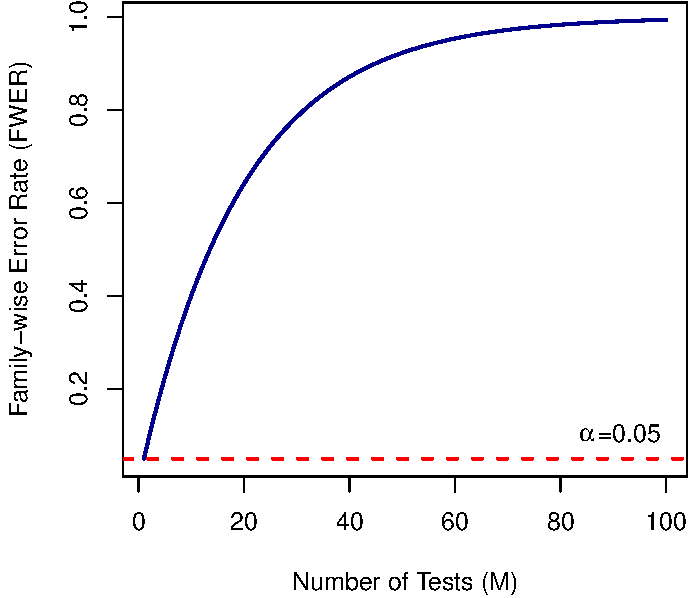
\includegraphics[width=0.5\textwidth]{FWER.pdf}
                  \caption{Family-Wise Error Rate Versus the Number of Hypothesis Tests, $M$.}\label{fig:FWER}
            \end{figure}
      \item A common value of $ M $ is $ \binom{m}{2} $: the number of pairwise comparisons necessary to compare each condition
            to every other condition.
            \begin{Example}{}{}
                  If $ m=5 $ and $ \alpha=0.05 $, then $ M=\binom{5}{2}=10 $. Therefore, $ \FWER=1-(1-0.05)^{10}=0.4013 $.
            \end{Example}
      \item Available to us are a variety of different statistical techniques that may be used to ensure the FWER
            does not exceed some threshold.
            \[ \FWER\le \alpha^\star \in[0,1] \]
            \begin{Remark}{General Notation}{}
                  \begin{itemize}
                        \item Denote the $ M $ null hypotheses as: $ \mathbf{H}_{0,1},\mathbf{H}_{0,2},\ldots,\mathbf{H}_{0,M} $.
                        \item Denote their corresponding $ p $-values as: $ p_1,p_2,\ldots,p_M $.
                  \end{itemize}
            \end{Remark}
            \begin{Example}{}{}
                  Suppose we test $ M =4 $ hypotheses, and the resulting $ p $-values are $ p_1 =0.015$, $ p_2=0.029 $,
                  $ p_3=0.008 $, and $ p_4=0.026 $.
            \end{Example}
\end{itemize}
\subsubsection*{The Bonferroni Correction}
\begin{itemize}
      \item This is the simplest method.
      \item Reject $ \mathbf{H}_{0,k} $ if
            \[ p_k\le \frac{\alpha^\star}{M} \quad\text{for }k=1,2,\ldots,M \]
            So, we test all $ M $ hypotheses at a significance level of $ \alpha^\star/M $.
      \item The procedure ensures $ \FWER\le \alpha^\star $. From Boole's Inequality,
            we know that
            \[ \FWER\le M\biggl(\frac{\alpha^\star}{M}\biggr)=\alpha^\star \]
      \item If we assume independence, the Bonferroni-corrected FWER becomes
            \[ 1-\biggl(1-\frac{\alpha^\star}{M} \biggr)^{\! M} \]
            Taking the limit of $ M \to\infty $ yields,
            \[ \lim\limits_{{M} \to {\infty}}\Biggl[1-\biggl(1-\frac{\alpha^\star}{M} \biggr)^{\! M}\Biggr]=1-e^{-\alpha^\star}  \]
            which for typical values of $ \alpha^\star $ in the range of $ \interval[open left]{0}{0.1} $ is approximately equal to $ \alpha^\star $.
            For example, if $ \alpha^\star=0.1 $, then the error is $ \approx 0.005 $. The asymptotic error rate
            and line of equality can be seen in~\Cref{fig:asymrate}.
            \begin{figure}[!htbp]
                  \centering
                  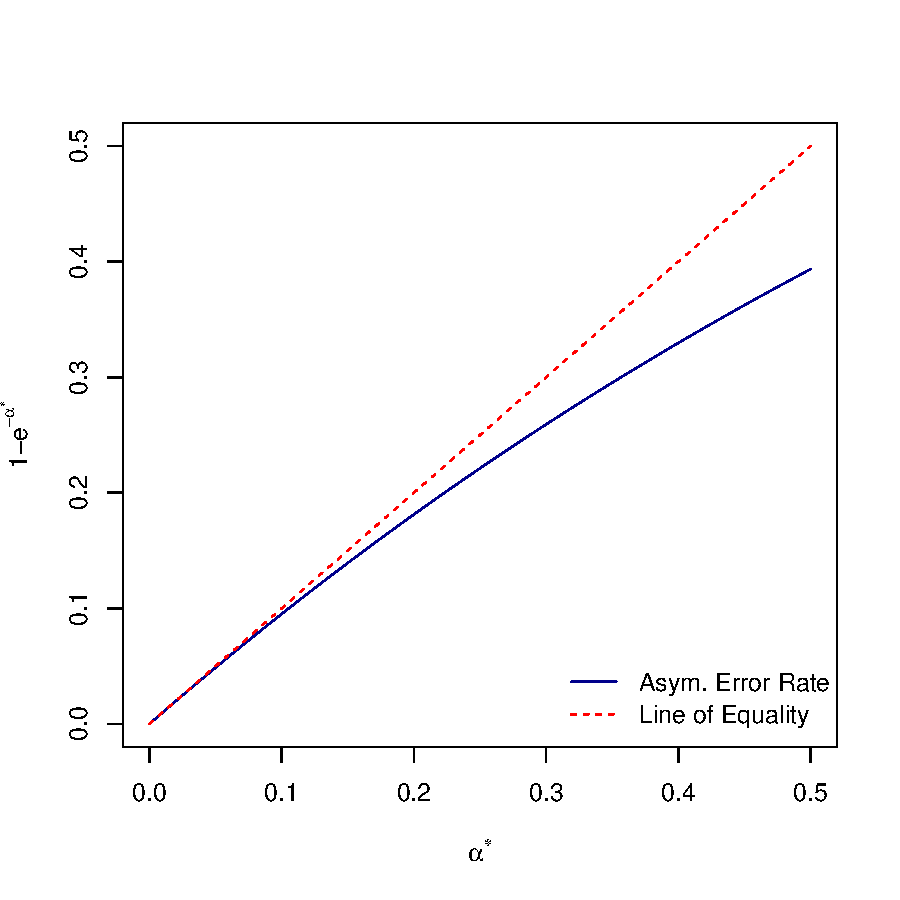
\includegraphics[width=0.5\textwidth]{asymrate.pdf}
                  \caption{Illustration of the Bonferroni Correction for Asymptotically Large $M$.}\label{fig:asymrate}
            \end{figure}
\end{itemize}
\begin{Example}{Four-test Example --- Bonferroni Correction}{}
      Let $ p_1=0.015 $, $ p_2=0.029 $, $ p_3=0.008 $, and $ p_4=0.026 $. Suppose that we wish to ensure
      $ \FWER\le \alpha^\star=0.05 $.

      \vspace{2mm}

      Under the Bonferroni Correction, we compare each
      $ p $-value to $ \alpha^\star/M=0.05/4=0.0125 $. Only $ p_3<0.0125 $, and hence
      only $ \mathbf{H}_{0,3} $ is rejected.
\end{Example}
\subsubsection*{The Šidák Correction}
\begin{itemize}
      \item This approach exploits the FWER formula derived when we assumed the $M$ tests were independent.
      \item Reject $ \mathbf{H}_{0,k} $ if
            \[ p_k\le 1-(1-\alpha^\star)^{1/M}\quad\text{for }k=1,2,\ldots,M \]
            \begin{Remark}{}{}
                  Where does the Šidák Correction come from?
                  \begin{align*}
                        \alpha^\star=\FWER=1-(1-\alpha)^M
                         & \iff 1-\alpha^\star = (1-\alpha)^M   \\
                         & \iff (1-\alpha^\star)^{1/M}=1-\alpha \\
                         & \iff \alpha=1-(1-\alpha^\star)^{1/M} \\
                  \end{align*}
            \end{Remark}
      \item This is actually not much different from the Bonferroni correction since
            \[ \frac{\alpha^\star}{M} \approx 1-(1-\alpha^\star)^{1/M} \]
            \begin{Example}{Bonferroni versus Šidák Correction}{}
                  Let $ \alpha^\star=0.05 $ and $ M=10 $. Then,
                  \[ \frac{\alpha^\star}{M} =0.005\quad\text{and}\quad 1-(1-\alpha^\star)^{1/M}=0.005116 \]
            \end{Example}
\end{itemize}
\begin{Example}{Four-test Example --- Šidák Correction}{}
      Let $ p_1=0.015 $, $ p_2=0.029 $, $ p_3=0.008 $, and $ p_4=0.026 $. Suppose that we wish to ensure
      $ \FWER\le \alpha^\star=0.05 $.

      \vspace{2mm}

      Under the Šidák Correction, we have
      \[ 1-(1-\alpha^\star)^{1/M}=1-(0.95)^{0.25}=0.012741 \]
      Therefore, we only reject $ \mathbf{H}_{0,3} $ since only $ p_3<0.012741 $.
\end{Example}
\subsubsection*{Holm's ``Step-Up'' Procedure}
\begin{itemize}
      \item The Bonferroni and Šidák corrections methods are very strict for large $M$.
            \begin{itemize}
                  \item In these cases \emph{most} null hypotheses will not be rejected.
                  \item If we're too strict, we basically stop rejecting null hypotheses thereby
                        eliminating Type I Errors, but we increase the Type II Errors.
            \end{itemize}
      \item Ideally we would have an approach that is less strict but still controls the FWER at some $ \alpha^\star $.
      \item This is exactly what Holm's Procedure gives us!
            \begin{framed}
                  \begin{enumerate}
                        \item Order the $M$ $p$-values from smallest to largest:
                              \[ p_{(1)},p_{(2)},\ldots,p_{(M)} \]
                              where $ p_{(k)} $ is the $ k^{\text{th}} $ smallest $ p $-value.
                        \item Starting from $ k=1 $ and continuing incrementally, compare
                              $ p_{(k)} $ to $ \alpha^\star/(M-k+1) $. Determine $ k^\star $,
                              the smallest value of $ k $ such that
                              \[ p_{(k)}>\frac{\alpha^\star}{M-k+1} \]
                        \item Reject the null hypotheses $ \mathbf{H}_{0,(1)},\ldots,\mathbf{H}_{0,(k^\star-1)} $
                              and do not reject $ \mathbf{H}_{0,(k^\star)},\ldots,\mathbf{H}_{0,(M)} $.
                  \end{enumerate}
            \end{framed}
      \item What's really happening?
            \begin{align*}
                  p_{(1)} & \text{ versus } \alpha^\star/M     \\
                  p_{(2)} & \text{ versus } \alpha^\star/(M-1) \\
                  p_{(3)} & \text{ versus } \alpha^\star/(M-2) \\
                          & \quad\;\vdots                      \\
                  p_{(M)} & \text{ versus } \alpha^\star
            \end{align*}
            We compare each $ p $-value to a Bonferroni-Corrected significance
            level based on the number of comparisons that remain to be
            made at a particular ``step.''
\end{itemize}
\begin{Theorem}{}{holm_FWER}
      Holm's procedure controls the family-wise error rate.
\end{Theorem}
\begin{Proof}{\Cref{thm:holm_FWER} \dagger}{}
      \begin{itemize}
            \item We need to show that $ \FWER=\Prob{V\ge 1}\le \alpha^\star\in[0,1] $ when using the Holm's procedure.
            \item Let $ p_{(1)},p_{(2)},\ldots,p_{(M)} $ be the ordered $ p $-values and let
                  $ \mathbf{H}_{0,(1)},\mathbf{H}_{0,(2)},\ldots,\mathbf{H}_{0,(M)} $ be the corresponding null hypotheses.
            \item Define $ K_0\subset \set{1,2,\ldots,M} $ to be the subset of indices which correspond
                  to true null hypotheses; that is, $ \mathbf{H}_{0,k} $ is true for $ k\in K_0 $.
            \item We can visualize the sequential decisions made in Holm's Procedure as follows:
                  \[ \overbracket{\underbracket{\mathbf{H}_{0,(1)}\cdots\mathbf{H}_{0,(h-1)}}_{\text{these are false $\mathbf{H}_0$'s}}\mathbf{H}_{0,(h)}\cdots \mathbf{H}_{0,(R)}}^{\text{these are rejected}}\mid \underbracket{\mathbf{H}_{0,(R+1)}\cdots\mathbf{H}_{0,(M)}}_{\text{these are not rejected}} \]
      \end{itemize}
      Let $ \mathbf{H}_{0,(h)} $ be the first \emph{true} $ \mathbf{H}_0 $ that was rejected. Since it was rejected by Holm's procedure, we know that
      \[ p_{(h)}\le \frac{\alpha^\star}{M-h+1} \]
      Also, clearly we must have $ h-1\le M-M_0 $ since $ M-M_0 $ is the total number of false $ \mathbf{H}_0 $'s and $ h-1 $ is the number of false
      $ \mathbf{H}_0 $'s encountered by test $ h $. And so,
      \[
            M_0\le M-h+1
            \iff \frac{1}{M_0} \ge \frac{1}{M-h+1}
            \iff \frac{\alpha^\star}{M_0} \ge \frac{\alpha^\star}{M-h+1}
      \]
      Thus, we must have $ p_{(h)}\le \alpha^\star/(M-h+1)\le \alpha^\star/M_0 $. Therefore,
      \begin{align*}
            \FWER
             & =\Prob*{V\ge 1}                                                                                                                    \\
             & =\Prob*{\text{At least one Type I Error in $M$ tests}}                                                                             \\
             & =\Prob*{\text{Reject at least one true $\mathbf{H}_0$}}                                                                            \\
             & =\Prob*{\exists\, k\in K_0\text{ such that }p_k\le \frac{\alpha^\star}{M_0}}                                                       \\
             & =\Prob*{\bigcup_{k\in K_0}p_k\le \frac{\alpha^\star}{M_0}}                                                                         \\
             & \le \sum_{k\in K_0}\Prob*{p_k\le \frac{\alpha^\star}{M_0}}                   &  & \text{by Boole's Inequality}                     \\
             & =\sum_{k\in K_0}\frac{\alpha^\star}{M_0}                                     &  & \!\!\!\!\begin{tabular}{l}
                  \text{since $p$-values for true null} \\
                  \text{hypotheses follow a $\uniform{0,1}$ distribution}
            \end{tabular}               \\
             & =M_0\biggl(\frac{\alpha^\star}{M_0}\biggr)                                   &  & \text{since the set $K_0$ has cardinality $M_0$} \\
             & =\alpha^\star
      \end{align*}
      Therefore, $ \FWER\le \alpha^\star $ as required.
\end{Proof}
\begin{Example}{Four-test Example ($ M=4 $) --- Holm's Procedure}{}
      Let $ p_1=0.015 $, $ p_2=0.029 $, $ p_3=0.008 $, and $ p_4=0.026 $. Suppose that we wish to ensure
      $ \FWER\le \alpha^\star=0.05 $.
      \begin{align*}
            p_{(1)}=p_3=0.008 & \text{ versus } \alpha^\star/M=0.05/4=0.0125     \\
            p_{(2)}=p_1=0.015 & \text{ versus } \alpha^\star/(M-1)=0.05/3=0.0167 \\
            p_{(3)}=p_4=0.026 & \text{ versus } \alpha^\star/(M-2)=0.05/2=0.025  \\
            p_{(4)}=p_2=0.029 & \text{ versus } \alpha^\star/(M-3)=0.05/1=0.05
      \end{align*}
      We reject $ \mathbf{H}_{0,(1)}=\mathbf{H}_{0,3} $ and $ \mathbf{H}_{0,(2)}=\mathbf{H}_{0,1} $. We do not reject
      $ \mathbf{H}_{0,(3)}=\mathbf{H}_{0,4} $ or $ \mathbf{H}_{0,(4)}=\mathbf{H}_{0,2} $. Note that $ k^\star=3 $.
\end{Example}
\begin{itemize}
      \item The decision process for all three of these methods can be visualized by plotting the ordered $p$-values
            $ p_{(k)} $ versus their ranks $ k=1,2,\ldots,M $ and overlay the significance thresholds which can
            be seen in~\Cref{fig:pvsrank1}.
            \begin{figure}[!htbp]
                  \centering
                  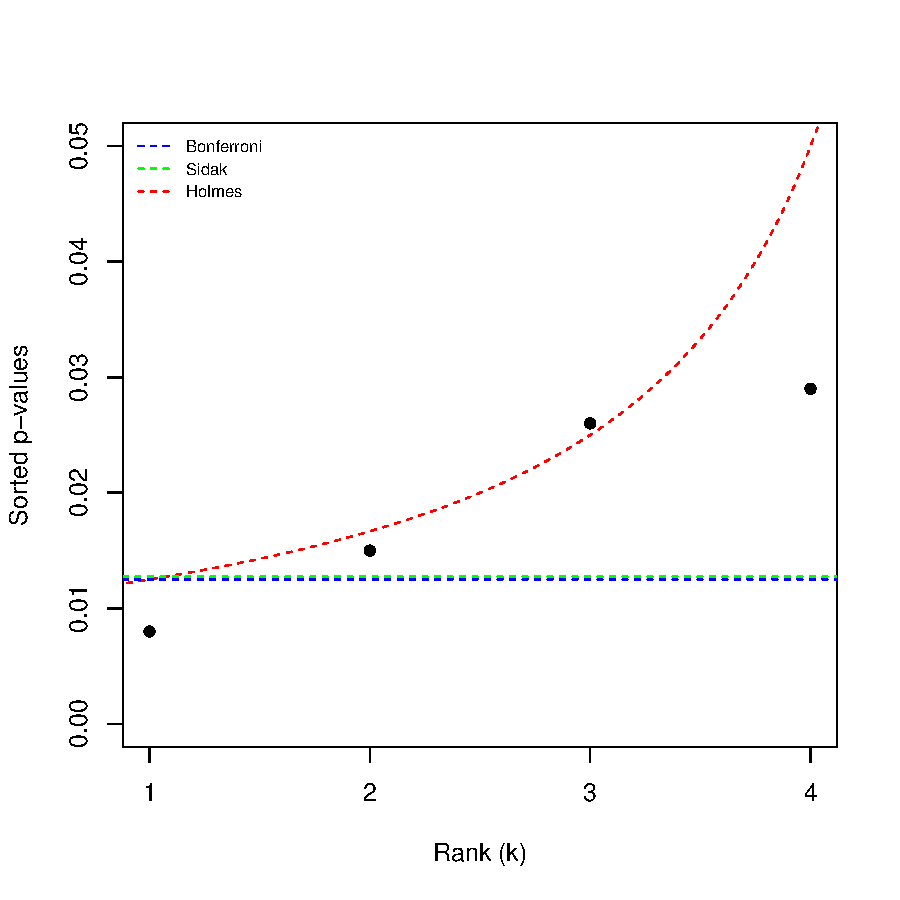
\includegraphics[width=0.5\textwidth]{pvsrank1.pdf}
                  \caption{Significance Thresholds for Several Methods of Correction (1).}\label{fig:pvsrank1}
            \end{figure}
      \item The Bonferroni correction is most strict, followed by the Šidák correction, then by Holm's procedure.
\end{itemize}
\subsubsection*{Adjusted $ p $-values}
\begin{itemize}
      \item So far we have framed each of the correction procedures above as an adjustment to the significance
            threshold against which each $p$-value is compared.
      \item Alternatively (and equivalently) we could invert this process and frame the decision in terms of a
            comparison of \emph{adjusted $p$-values} to $ \alpha^\star $.
      \item This is more familiar (compare our $ p $-values to some constant threshold $ \alpha^\star $).
            \begin{itemize}
                  \item We just need to adjust our $p$-values first.
            \end{itemize}
      \item The decisions made with the following adjusted $p$-values are identical to that achieved by comparing
            unadjusted $p$-values to the methods' adjusted significance thresholds.
            \begin{itemize}
                  \item Bonferroni: Reject $ \mathbf{H}_{0,k} $ if $ p_k^\star\le \alpha^\star $ where
                        \[ p_k^\star=Mp_k \]
                        \begin{Example}{Bonferroni's Adjusted $ p $-values}{}
                              In our four-test example, $ p_1^\star=0.06 $, $ p_2^\star=0.116 $, $ p_3^\star=0.032 $, and $ p_4^\star=0.104 $.
                              Comparing to $ \alpha^\star=0.05 $, we reject $ \mathbf{H}_{0,3} $.
                        \end{Example}
                  \item Šidák: Reject $ \mathbf{H}_{0,k} $ if $ p_k^\star\le \alpha^\star $ where
                        \[ p_k^\star=1-(1-p_k)^M \]
                        \begin{Example}{Šidák's Adjusted $ p $-values}{}
                              In our four-test example, $ p_1^\star=0.0587 $, $ p_2^\star=0.111 $, $ p_3^\star=0.0316 $, and $ p_4^\star=0.1 $.
                              Comparing to $ \alpha^\star=0.05 $, we reject $ \mathbf{H}_{0,3} $.
                        \end{Example}
                  \item Holm: Reject $ \mathbf{H}_{0,k} $ if $ p_{(k)}^\star\le \alpha^\star $ where
                        \[ p_{(k)}^\star=\max_{j\le k}\set*{p_{(j)}(M-j+1)} \]
                        \begin{Example}{Holm's Adjusted $ p $-values}{}
                              Let $ p_1=0.015 $, $ p_2=0.029 $, $ p_3=0.008 $, and $ p_4=0.026 $.
                              \[ \begin{array}{ccccl}
                                          k & p_{(k)} & M-k+1 & p_{(k)}(M-k+1) & p_{(k)}^\star=\max_{j\le k}\set*{p_{(j)}(M-j+1)}      \\
                                          \midrule
                                          1 & 0.008   & 4     & 0.032          & \max\set{0.032}=0.032=p_{(1)}^\star                   \\
                                          2 & 0.015   & 3     & 0.045          & \max\set{0.032,0.045}=0.045=p_{(2)}^\star             \\
                                          3 & 0.026   & 2     & 0.052          & \max\set{0.032,0.045,0.052}=0.052=p_{(3)}^\star       \\
                                          4 & 0.029   & 1     & 0.029          & \max\set{0.032,0.045,0.052,0.029}=0.052=p_{(4)}^\star
                                    \end{array} \]
                              Thus, $ p_1^\star=p_{(2)}^\star=0.045 $, $ p_2^\star=p_{(4)}^\star=0.052 $, $ p_3^\star=p_{(1)}^\star=0.032 $, and
                              $ p_4^\star=p_{(3)}^\star=0.052 $. Comparing to $ \alpha^\star=0.05 $, we reject
                              $ \mathbf{H}_{0,1} $ and $ \mathbf{H}_{0,3} $.
                        \end{Example}
            \end{itemize}
      \item Implemented in R with \code{p.adjust()}.
\end{itemize}
\subsection{False Discovery Rate}
\begin{itemize}
      \item In the mid-1900s, Statisticians developed FWER methods with $ M\approx 20 $ comparisons in mind.
      \item In the era of Big Data, much larger values of $M$ are typical.
      \item For larger values of $M$, traditional methods tend to be very conservative, and so FWER is perhaps
            not the best metric to control.
      \item More recently, emphasis has been placed on controlling the \emph{rate} at which Type I Errors occur.
            \begin{Definition}{False discovery proportion}{}
                  The \textbf{false discovery proportion} (FDP) is
                  \[ Q=\frac{V}{R} \]
                  Thus, $ Q $ is the proportion of all rejected null hypotheses that were rejected
                  in error.
            \end{Definition}
      \item In particular, interest lies in controlling the \textbf{false discovery rate} (FDR).
            \begin{Definition}{False discovery rate}{}
                  The \textbf{false discovery rate} is
                  \[ \E{Q}=\E*{\frac{V}{R}} \]
            \end{Definition}
      \item Unlike the FWER, the FDR is adaptive in the sense that the number of Type I Errors $V$ has different
            implications depending on the size of $M$. That is,
            \begin{itemize}
                  \item Two Type I Errors in 10 tests might be unacceptable.
                  \item Two Type I Errors in 100 tests might be okay.
            \end{itemize}
      \item Methods that control the FDR are less strict than methods that control FWER\@.
            \begin{itemize}
                  \item More Type I Errors will occur with such methods, but this is viewed as acceptable when $M$ is
                        very large.
            \end{itemize}
\end{itemize}
\subsubsection*{Benjamini-Hochberg Procedure}
\begin{itemize}
      \item The Benjamini-Hochberg (BH) procedure for controlling FDR is a sequentially rejective procedure
            much like Holm's procedure for controlling FWER\@. The main difference is the threshold we
            compare the ordered $ p $-values to.
      \item We summarize the BH procedure, which aims to ensure $ \text{FDR}\le \alpha^\star $:
            \begin{framed}
                  \begin{enumerate}
                        \item Order the $M$ $p$-values from smallest to largest:
                              \[ p_{(1)},p_{(2)},\ldots,p_{(M)} \]
                              where $ p_{(k)} $ is the $ k^{\text{th}} $ smallest $ p $-value.
                        \item Starting from $ k=1 $ and continuing incrementally, compare
                              $ p_{(k)} $ to $ k\alpha^\star/M $. Determine $ k^\star $
                              the largest value of $ k $ such that
                              \[ p_{(k)}\le \frac{k\alpha^\star}{M}  \]
                        \item Reject the null hypotheses $ \mathbf{H}_{0,(1)},\ldots,\mathbf{H}_{0,(k^\star)} $
                              and do not reject $ \mathbf{H}_{0,(k^\star+1)},\ldots,\mathbf{H}_{0,(M)} $.
                  \end{enumerate}
            \end{framed}
      \item The decision process associated with this procedure is best visualized with a plot of the ordered $p$-values
            $ p_{(k)} $ versus their ranks $ k=1,2,\ldots,M $ with the significance threshold overlaid which can
            be seen in~\Cref{fig:pvsrank2}.
            \begin{itemize}
                  \item The BH significance threshold is the line with intercept $0$ and slope $ \alpha^\star/M $.
            \end{itemize}
            \begin{figure}[!htbp]
                  \centering
                  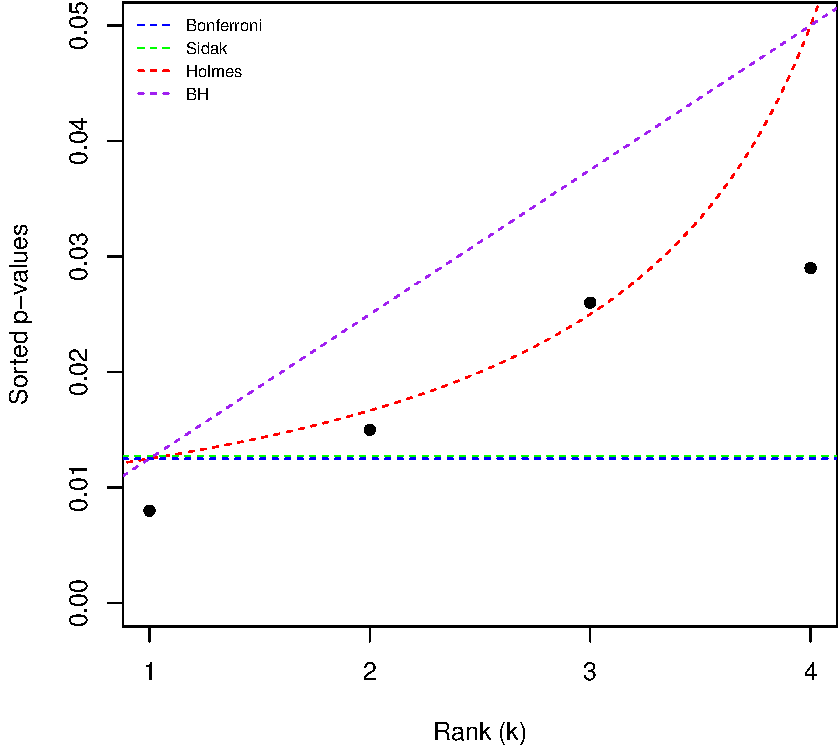
\includegraphics[width=0.5\textwidth]{pvsrank2.pdf}
                  \caption{Significance Thresholds for Several Methods of Correction (2).}\label{fig:pvsrank2}
            \end{figure}
            \begin{Example}{Four-test Example --- Benjamini-Hochberg Procedure}{}
                  Let $ p_1=0.015 $, $ p_2=0.029 $, $ p_3=0.008 $, and $ p_4=0.026 $. Suppose that we wish to ensure
                  $ \FWER\le \alpha^\star=0.05 $. Since all $ p $-values fall below the purple line in~\Cref{fig:pvsrank2},
                  we reject all four null hypotheses.
            \end{Example}
      \item This threshold is much less strict than any of the FWER-control thresholds, but this is the appeal of
            the approach.
      \item The procedure that guarantees $ \text{FDR}\le \alpha^\star $ is beyond the scope of this course.
            However, the proof can be found in~\citet{benjamini} and~\citet{storey}.
      \item Like the FWER controlling methods we can define Benjamini-Hochberg-adjusted $p$-values and invert
            the decision framework by comparing the adjusted $ p $-values to $ \alpha^\star $.
            \begin{itemize}
                  \item Reject $ \mathbf{H}_{0,(k)} $ if $ p_{(k)}^\star\le \alpha^\star $ where
                        \[ p_{(k)}^\star=\min_{j\ge k}\set*{\frac{Mp_{(j)}}{j}} \]
                        \begin{Example}{Benjamini-Hochberg Procedure's Adjusted $ p $-values}{}
                              Let $ p_1=0.015 $, $ p_2=0.029 $, $ p_3=0.008 $, and $ p_4=0.026 $.
                              \[ \begin{array}{cccl}
                                          k & p_{(k)} & M p_{(k)}/k & p_{(k)}^\star=\min_{j\ge k}\set*{Mp_{(j)}/j}          \\
                                          \midrule
                                          1 & 0.008   & 0.032       & \min\set{0.032,0.030,0.035,0.029}=0.029=p_{(1)}^\star \\
                                          2 & 0.015   & 0.030       & \min\set{0.030,0.035,0.029}=0.029=p_{(2)}^\star       \\
                                          3 & 0.026   & 0.035       & \min\set{0.035,0.029}=0.029=p_{(3)}^\star             \\
                                          4 & 0.029   & 0.029       & \min\set{0.029}=0.029=p_{(4)}^\star
                                    \end{array} \]
                              Thus, $ p_1^\star=p_{(2)}^\star=0.029 $, $ p_2^\star=p_{(4)}^\star=0.029 $, $ p_3^\star=p_{(1)}^\star=0.029 $,
                              and $ p_4^\star=p_{(3)}^\star=0.029 $. Comparing to $ \alpha^\star=0.05 $,
                              we reject all $ \mathbf{H}_{0} $'s.
                        \end{Example}
            \end{itemize}
\end{itemize}
\href{https://github.com/Hextical/university-notes/blob/master/year-3/semester-3/STAT 430/code/W4/Multiple_testing_example.R}{[R Code] \texttt{Multiple\_testing\_example}}
\subsection{Sample Size Determination}
\begin{itemize}
      \item So what does all of this mean for power analyses and sample size calculations?
      \item There is a duality between significance level and power.
            \begin{itemize}
                  \item All else equal, reducing a test's significance level will increase the Type II Error rate and hence
                        decrease power.
                  \item Play around with \href{https://nathaniel-t-stevens.shinyapps.io/ErrorIllustrator/}{this interactive app} to gain comfort with this notion.
                        \begin{itemize}
                              \item Assume $ \mathcal{R}=\set*{t\mid t\ge z_\alpha} $.
                              \item Recall that: \begin{itemize}
                                          \item $ \alpha=\Prob*{\text{Type I Error}}=\Prob*{T\in\mathcal{R}\given \text{$ \mathbf{H}_0 $ is true}}=\Prob*{T\ge z_\alpha\given \text{$ \mathbf{H}_0 $ is true}}$.
                                          \item $ \beta=\Prob*{\text{Type II Error}}=\Prob*{T\notin\mathcal{R}\given \text{$ \mathbf{H}_\text{A} $ is true}}=\Prob*{T< z_\alpha\given \text{$ \mathbf{H}_\text{A} $ is true}} $.
                                    \end{itemize}
                        \end{itemize}
            \end{itemize}
      \item Thus, all the correction procedures discussed (which decrease the effective significance level)
            negatively impact power.
      \item In order to maintain power at some pre-specified level, we must compensate by increasing the sample
            size.
      \item Therefore, the more complicated your experiment (i.e., the more conditions it has), the larger your
            sample sizes will need to be.
            \begin{itemize}
                  \item Such modifications can be accounted for when selecting a sample size.
                  \item The significance level you use in your sample size calculations should be the adjusted one based
                        on the correction method you use.
                  \item This is easier to do with \emph{some} correction methods than others.
            \end{itemize}
\end{itemize}

\makeheading{Week 5}
\section*{Primer on Logistic Regression}
\begin{itemize}
      \item Linear regression is an effective method of modelling the relationship between a single response variable
            $ Y $, and one or more explanatory variables $ (x_1,x_2,\ldots,x_p) $.
            \begin{itemize}
                  \item However, ordinary linear regression assumes that the response variable follows a normal distribution
                        (i.e., $ Y \sim \N{\mu,\sigma^2} $).
                  \item When the response variable is binary, this assumption is no longer valid.
            \end{itemize}
      \item When we have a binary response, the Bernoulli distribution (i.e., $ Y \sim \bin{1,\pi} $) is a much more
            appropriate distributional assumption.
            \begin{itemize}
                  \item But ordinary linear regression is no longer appropriate.
                  \item Instead, we use \textbf{Logistic Regression}.
            \end{itemize}
      \item In the context of a linear regression model, the expected response (given
            the values of the explanatory variables) is equated to the \textbf{linear predictor} $ \beta_0+\beta_1x_1+\cdots+\beta_p x_p $:
            \[ \E{Y\given x_1,x_2,\ldots,x_p}=\mu=\beta_0+\beta_1x_1+\cdots+\beta_p x_p \]
      \item In the context of Logistic Regression we also want to relate the expected response to the linear predictor.
            \begin{itemize}
                  \item But now, $ \E{Y}=\pi\in[0,1] $.
                  \item And equating $ \pi $ and $ \beta_0+\beta_1 x_1+\cdots+\beta_p x_p $ does not make sense. In general, the linear predictor need not lie in $ [0,1] $.
                        \[ \pi=\beta_0+\beta_1x_1+\cdots+\beta_p x_p\quad\text{not a good thing to do} \]
            \end{itemize}
      \item Instead, we relate the linear predictor to $ \E{Y}=\pi $ through a monotonic differentiable \textbf{link function} that maps $ [0,1]\to\mathbf{R} $.
            \begin{itemize}
                  \item Logistic Regression arises when this link function is the \textbf{logit} function:
                        \[ \text{logit}(\pi)=\log*{\frac{\pi}{1-\pi}}=\beta_0+\beta_1x_1+\cdots+\beta_p x_p \]
                  \item Inverting this yields the expected response (given the values of the explanatory variables):
                        \[ \widehat{\E{Y\given x_1,x_2,\ldots,x_p}}=\hat{\pi}=\frac{e^{\hat{\beta}_0+\hat{\beta}_1 x_1+\cdots+\hat{\beta}_p x_p}}{1+e^{\hat{\beta}_0+\hat{\beta}_1 x_1+\cdots+\hat{\beta}_p x_p}}
                              =\text{expit}(\beta_0+\beta_1x_1+\cdots+\beta_p x_p)  \]
            \end{itemize}
      \item To interpret $ \beta_0 $, we set each explanatory variable to zero (i.e., $ x_1=x_2=\cdots=x_p=0 $).
            \begin{itemize}
                  \item We see that $ \beta_0 $ is the \textbf{log-odds} that $ Y=1 $ when $ x_1=x_2=\cdots=x_p=0 $.
                        \[ \log*{\frac{\pi}{1-\pi}}=\beta_0 \]
                  \item Equivalently, $ e^{\beta_0} $ is the \textbf{odds} that the response would equal $ 1 $ when $ x_1=x_2=\cdots=x_p=0 $.
                        Exponentiating both sides yields
                        \[ \frac{\pi}{1-\pi}=e^{\beta_0}  \]
            \end{itemize}
      \item The interpretation of $\beta_j$, for $ j=1,2,\ldots,p $, is uncovered by considering the Logistic Regression equation
            for different values of $ x_j $.
            \begin{itemize}
                  \item Let $ \pi_x $ be the value of $ \pi $ when $ x_j=x $ and let $ \pi_{x+1} $ be the value of $ \pi $ when $ x_j=x+1 $.
                        \begin{align*}
                              \log*{\frac{\pi_{x+1}}{1-\pi_{x+1}}}-\log*{\frac{\pi_x}{1-\pi_x}}
                               & =(\beta_0+\beta_1x_1+\cdots+\beta_j(x+1)+\cdots+\beta_p x_p) \\
                               & \quad\quad-(\beta_0+\beta_1x_1+\cdots+\beta_j x+\beta_p x_p) \\
                               & =\beta_j
                        \end{align*}
                  \item Thus:
                        \[ \log*{\frac{\pi_{x+1}}{1-\pi_{x+1}}\Bigg/\frac{\pi_x}{1-\pi_x}}=\beta_j \]
                        and so $ \beta_j $ is interpreted as a \textbf{log-odds ratio}, comparing the odds that $ Y=1 $
                        when $ x_j=x+1 $ versus $ x_j=x $ (all else being equal).
                  \item Equivalently, $ e^{\beta_j} $ is interpreted as the \textbf{odds ratio}, comparing the odds that
                        $ Y=1 $ when $ x_j=x+1 $ versus $ x_j=x $ (all else being equal). Exponentiating yields
                        \[ \frac{\pi_{x+1}}{1-\pi_{x+1}} \Bigg/ \frac{\pi_x}{1-\pi_x} =e^{\beta_j} \]
            \end{itemize}
      \item \textbf{Maximum likelihood estimation} is a method that is used to estimate parameters in Logistic Regression.
            \begin{itemize}
                  \item This means that the $ \hat{\beta} $'s are maximum likelihood estimates, whose corresponding estimators have nice properties, such as:
                        \[ \tilde{\beta}\stackrel{\cdot}{\sim}\N*{\beta,\frac{1}{J(\beta)}} \]
                        where $ J(\beta) $ is the Fisher Information.
                  \item A consequence of this is that hypotheses of the form
                        \begin{tightcenter}
                              $ \mathbf{H}_0 $: $ \beta_j =0 $ versus $ \mathbf{H}_\text{A} $: $ \beta_j\ne 0 $
                        \end{tightcenter}
                        are done with $ Z $-\emph{tests} with test statistics given by
                        \[ t=\frac{\hat{\beta}_j-0}{\Se*{\hat{\beta}_j}}\stackrel{\cdot}{\sim}\N{0,1}  \]
                  \item In order to test hypotheses about several $ \beta $'s being simultaneously equal to zero, we use \emph{likelihood ratio tests}.
            \end{itemize}
\end{itemize}
\chapter{Blocking}
\begin{itemize}
      \item In the context of designed experiments we categorize factors as either:
            \begin{itemize}
                  \item \emph{Design} factors: we manipulate these to quantify their impact on the response.
                        They define the experimental conditions.
                  \item \emph{Allowed-to-vary} factors: these are unknown or known but uncontrollable and thus
                        are \underline{not} controlled in the experiment.
                  \item \emph{Nuisance} factors: we control these to eliminate their effect on the response.
            \end{itemize}
      \item But remember: in practice, context dictates whether a factor should be considered a design factor, a
            nuisance factor, or if it should be allowed to vary.
\end{itemize}
\begin{figure}[!htbp]
      \centering
      
\includegraphics[width=0.8\textwidth]{browsers.pdf}
      \caption{Four Levels of the \emph{browser} Factor.}
\end{figure}
\begin{enumerate}
      \item Usability testing involves studying the ease with which an individual uses a product or service
            for some intended purpose. Suppose investigators are performing a usability test to determine
            with which browser 70 to 80-year-old users find it easiest to look up the phone number of
            the nearest pharmacy. In this example, experimental units (70 to 80-year-olds) are randomly
            assigned to one of four browser conditions, and the investigators measure the time it
            takes to complete the task.
            \begin{itemize}
                  \item Browser is the design factor.
            \end{itemize}
      \item Suppose that Netflix is experimenting with server-side modifications to improve (reduce) the
            latency of Netflix.com. We hypothesize that the current infrastructure serves as a control condition
            and the modified infrastructure reduces median page load time. It is possible
            that a user's browser may also affect page load time, but this effect is not of interest to
            the investigators. To control for the potential impact of one's browser, Netflix initially
            experiments with only Firefox users.
            \begin{itemize}
                  \item Browser is the nuisance factor.
            \end{itemize}
      \item Suppose that Amazon.ca is experimenting with the width of their search bar. They hypothesize
            that a wider search bar will minimize the amount of mouse movement required to
            navigate to it, thereby minimizing the average time-to-query. The experimenters do not care
            which browser a customer uses and so this factor is uncontrolled and hence is \emph{allowed-to-vary}
            during their experiment.
            \begin{itemize}
                  \item Browser is the allowed-to-vary factor.
            \end{itemize}
\end{enumerate}
\begin{itemize}
      \item It's also important to understand the subtle distinction between nuisance factors and design factors in
            the context of a single experiment.
            \begin{itemize}
                  \item We control both factors in the experiment.
                  \item With a design factor we wish to quantify its influence on the response variable.
                  \item With a nuisance factor we do not care to quantify its effect, we wish only to \emph{eliminate} it.
            \end{itemize}
      \item We eliminate the effect of one or more nuisance factors with \textbf{blocking}.
            \begin{itemize}
                  \item To eliminate the effect of a nuisance factor, it cannot be allowed to vary on its own.
                  \item Blocking fixes the nuisance factor at one or more levels (\textbf{blocks}).
                  \item By holding a nuisance factor fixed, it cannot vary and hence cannot influence the response.
                        \begin{itemize}
                              \item This is how Netflix handled the nuisance factor ``browser'' in Example 2.
                        \end{itemize}
            \end{itemize}
\end{itemize}
\section{Randomized Complete Block Designs}
\begin{itemize}
      \item The randomized complete block design (RCBD) is a simple experimental design that may be applied
            when we wish to investigate.
            \begin{itemize}
                  \item A single design factor; e.g., $ m $ levels, $ m $ conditions.
                  \item While controlling for a single nuisance factor; e.g., $ b $ levels, $ b $ blocks.
            \end{itemize}
      \item In a RCBD, we carry out each of the experimental conditions in every one of the blocks.
            \begin{itemize}
                  \item $ m $ conditions happening inside each of $ b $ blocks.
            \end{itemize}
      \item The observed data in such an experiment is $ y_{ijk} $.
            \begin{itemize}
                  \item Response observation for unit $ i=1,2,\ldots,n_{jk} $ in condition $ j=1,2,\ldots,m $
                        within block $ k=1,2,\ldots,b $.
            \end{itemize}
      \item We assume that there are $n_{jk}$ units in $ (\text{condition}, \text{block}) = (j, k) $ and thus an overall total of
            $ N=\sum_{k=1}^{b} \sum_{j=1}^{m} n_{jk} $ units.
            \begin{itemize}
                  \item If $ n_{jk}=n $ for all $ (j,k) $, we call the design ``balanced.''
            \end{itemize}
      \item We tabulate the response data of this form below:
            \begin{table}[!htbp]
                  \centering
                  \caption{Response Observations in a Randomized Complete Block Design}
                  \begin{NiceTabular}{cc|cccc|c}
                        \multicolumn{2}{c}{}       & \multicolumn{4}{c}{\emph{Block}} &                                                                                                                                                                                                                           \\
                        \multicolumn{2}{c}{}       & $1$                                & $2$                                              & $\cdots$                                         & $b$      & \multicolumn{1}{c}{}                                                                                     \\
                        \cmidrule{2-7}
                        \multirow{4}{*}{\emph{Condition}} & $1$                                & $\set{y_{i11}}_{i=1}^{n_{11}}$                   & $\set{y_{i12}}_{i=1}^{n_{12}}$                   & $\cdots$ & $\set{y_{i1b}}_{i=1}^{n_{1b}}$                   & $\bar{y}_{\bullet 1\bullet}$                          \\
                        & $2$                                & $\set{y_{i21}}_{i=1}^{n_{21}}$                   & $\set{y_{i22}}_{i=1}^{n_{22}}$                   & $\cdots$ & $\set{y_{i2b}}_{i=1}^{n_{2b}}$                   & $\bar{y}_{\bullet 2\bullet}$                          \\
                        & $\vdots$                           & $\vdots$                                         & $\vdots$                                         & $\ddots$ & $\vdots$                                         & $\vdots$                                              \\
                        & $m$                                & $\set{y_{im1}}_{i=1}^{n_{m1}}$                   & $\set{y_{im2}}_{i=1}^{n_{m2}}$                   & $\cdots$ & $\set{y_{imb}}_{i=1}^{n_{mb}}$                   & $\bar{y}_{\bullet m\bullet}$                          \\
                        \cmidrule{2-7}
                        \multicolumn{1}{c}{}       & \multicolumn{1}{c}{}               & \multicolumn{1}{c}{$\bar{y}_{\bullet\bullet 1}$} & \multicolumn{1}{c}{$\bar{y}_{\bullet\bullet 2}$} & $\cdots$ & \multicolumn{1}{c}{$\bar{y}_{\bullet\bullet b}$} & \multicolumn{1}{c}{$\bar{y}_{\bullet\bullet\bullet}$}
                  \end{NiceTabular}
            \end{table}
            \begin{itemize}
                  \item Block-specific average responses: $\bar{y}_{\bullet\bullet 1},\bar{y}_{\bullet\bullet 2},\ldots,\bar{y}_{\bullet\bullet b}$.
                  \item Overall average response: $\bar{y}_{\bullet\bullet\bullet}$.
                  \item Condition-specific average responses: $\bar{y}_{\bullet 1\bullet},\bar{y}_{\bullet 2\bullet},\ldots,\bar{y}_{\bullet m\bullet}$.
            \end{itemize}
      \item We calculate the row, column, and overall means as follows:
            \[ \bar{y}_{\bullet j\bullet}=\frac{1}{b} \sum_{k=1}^{b} \bar{y}_{\bullet jk} \]
            \[ \bar{y}_{\bullet\bullet k}=\frac{1}{m} \sum_{j=1}^{m} \bar{y}_{\bullet jk} \]
            \[ \bar{y}_{\bullet\bullet\bullet}=\frac{1}{N} \sum_{k=1}^{b} \sum_{j=1}^{m} n_{jk}\bar{y}_{\bullet jk}=\frac{1}{N} \sum_{k=1}^{b} \sum_{j=1}^{m} \sum_{i=1}^{n_{jk}} y_{ijk} \]
            where $ \bar{y}_{\bullet jk} $ is the average response in $  (\text{condition}, \text{block}) $ cell $ (j, k) $, also
            \[ \bar{y}_{\bullet jk}=\frac{1}{n_{jk}} \sum_{i=1}^{n_{jk}} y_{ijk} \]
      \item Simple summaries such as these provide a crude assessment of whether the condition-to-condition and
            block-to-block variation is large.
            \begin{itemize}
                  \item If the condition-specific averages are very different, this suggests that the design factor influences the response.
                  \item If the block-specific averages are very different, this suggests that the nuisance factor influences the response, and that blocking was appropriate.
            \end{itemize}
      \item The primary analysis goal in a RCBD is to determine whether the expected response differs significantly
            from one condition to another.
            \begin{itemize}
                  \item And if so, to identify the optimal condition.
                  \item While controlling for the potential effect of the nuisance factor.
            \end{itemize}
      \item We've previously done this with gatekeeper tests of the form:
            \begin{tightcenter}
                  $ \mathbf{H}_0 $: $ \theta_1=\theta_2=\cdots=\theta_m $ versus $ \mathbf{H}_\text{A} $: $ \theta_j\ne \theta_k $ for some $ j\ne k $
            \end{tightcenter}
      \item We do the same thing here, while accounting for the nuisance factor, with \emph{appropriately defined} linear (continuous response)
            or logistic (binary response) regression models which contain:
            \begin{itemize}
                  \item An intercept.
                  \item $ m-1 $ indicator variables for the design factor's levels.
                  \item $ b-1 $ indicator variables for the nuisance factor's levels.
            \end{itemize}
      \item We write the linear predictor as:
            \begin{equation}\tag{$\star$}
                  \alpha+\sum_{j=1}^{m-1} \beta_j x_{ij}+\sum_{k=1}^{b-1} \gamma_k z_{ij}\label{lpeqn}
            \end{equation}
            \begin{itemize}
                  \item $ x_{ij}=1 $ if unit $ i $ is in condition $ j $, and zero otherwise.
                  \item $ z_{ik}=1 $ if unit $ i $ is in block $ k $, and zero otherwise.
                  \item The $ \beta $'s jointly quantify the effect of the design factor.
                  \item The $ \gamma $'s jointly quantify the effect of the nuisance factor.
            \end{itemize}
      \item Two relevant hypotheses are:
            \begin{enumerate}[(1)]
                  \item $ \mathbf{H}_0 $: $ \beta_1=\beta_2=\cdots=\beta_{m-1} $ versus $ \mathbf{H}_\text{A} $: $ \beta_j\ne 0 $ for some $ j $.
                        \begin{itemize}
                              \item If we don't reject $ \mathbf{H}_0 $, this suggests the $ x $'s don't need to be in the model
                                    and hence the design factor doesn't significantly influence the response.
                        \end{itemize}
                  \item $ \mathbf{H}_0 $: $ \gamma_1=\gamma_2=\cdots=\gamma_{b-1} $ versus $ \mathbf{H}_\text{A} $: $ \gamma_k\ne 0 $ for some $ k $.
                        \begin{itemize}
                              \item If we don't reject $ \mathbf{H}_0 $, this suggests the $ z $'s don't need to be in the model
                                    and hence the nuisance factor doesn't significantly influence the response. Therefore, blocking wasn't necessary.
                        \end{itemize}
            \end{enumerate}
      \item We test these hypotheses by comparing a \emph{full} model and \emph{reduced} models where the \emph{full} model
            is a model with a linear predictor given by~(\ref{lpeqn}), and a \emph{reduced} model is a model with a linear predictor that arises by $ \mathbf{H}_0 $
            being true.
            \begin{itemize}
                  \item We try to determine whether the full model fits the data significantly better than the reduced one.
            \end{itemize}
\end{itemize}
\subsection{RCBD to Compare Means}
\begin{itemize}
      \item Here, we're interested in testing the following hypothesis (while accounting for the influence of the
            nuisance factor):
            \begin{tightcenter}
                  $ \mathbf{H}_0 $: $ \mu_1=\mu_2=\cdots=\mu_m $ versus $ \mathbf{H}_\text{A} $: $ \mu_j\ne \mu_k $ for some $ j\ne k $.
            \end{tightcenter}
      \item We do this by testing:
            \begin{tightcenter}
                  $ \mathbf{H}_0 $: $ \beta_1=\beta_2=\cdots=\beta_{m-1} $ versus $ \mathbf{H}_\text{A} $: $ \beta_j\ne 0 $ for some $ j $
            \end{tightcenter}
            with an ANOVA in the context of the following linear regression model.
            \[ Y_i=\alpha+\sum_{j=1}^{m-1} \beta_j x_{ij}+\sum_{k=1}^{b-1} \gamma_k z_{ij}+\varepsilon_i \]
            where $ Y_i $ is the response observation for unit $ i=1,2,\ldots,N=\sum_{k=1}^{b} \sum_{j=1}^{m} n_{jk} $
            and $ \varepsilon_i \stackrel{\text{iid}}{\sim}\N{0,\sigma^2} $ is a random error term.
      \item We show the relevant ANOVA table below:
            \begin{table}[!htbp]
                  \centering
                  \caption{Two-Way ANOVA Table Associated With a Randomized Complete Block Design}
                  \begin{NiceTabular}{|l|c|c|c|c|}
                        \toprule
                        Source    & SS                     & d.f.        & MS                                                                   & Test Statistic                                           \\
                        \midrule
                        Condition & $ \text{SS}_\text{C} $ & $ m-1 $     & $ \text{MS}_\text{C}=\text{SS}_\text{C}/(m-1) $     & $ t_\text{C}=\text{MS}_\text{C}/\text{MS}_\text{E} $ \\
                        Block     & $ \text{SS}_\text{B} $ & $ b-1 $     & $ \text{MS}_\text{B}=\text{SS}_\text{B}/(b-1) $     & $ t_\text{B}=\text{MS}_\text{B}/\text{MS}_\text{E} $ \\
                        Error     & $ \text{SS}_\text{E} $ & $ N-m-b+1 $ & $ \text{MS}_\text{E}=\text{SS}_\text{E}/(N-m-b+1) $ &                                                      \\
                        \midrule
                        Total     & $ \text{SS}_\text{T} $ & $ N-1 $\\
                        \bottomrule
                  \end{NiceTabular}
            \end{table}
      \item The sums of squares given in the table are:
            \begin{itemize}
                  \item Total sum of squares (quantifies overall response variation):
                        \[ \text{SS}_\text{T}=\sum_{k=1}^{b} \sum_{j=1}^{m} \sum_{i=1}^{n_{jk}} (y_{ijk}-\bar{y}_{\bullet\bullet\bullet})^2=\text{SS}_\text{C}+\text{SS}_\text{B}+\text{SS}_\text{E} \]
                  \item Condition sum of squares (quantifies condition-to-condition response variation):
                        \[ \text{SS}_\text{C}=\sum_{k=1}^{b} \sum_{j=1}^{m} \sum_{i=1}^{n_{jk}} (\bar{y}_{\bullet j\bullet}-\bar{y}_{\bullet\bullet\bullet})^2 \]
                  \item Block sum of squares (quantifies block-to-block response variation):
                        \[ \text{SS}_\text{B}=\sum_{k=1}^{b} \sum_{j=1}^{m} \sum_{i=1}^{n_{jk}}(\bar{y}_{\bullet\bullet k}-\bar{y}_{\bullet\bullet\bullet})^2   \]
                  \item Error sum of squares (quantifies residual response variation not accounted for by conditions of blocks):
                        \[ \text{SS}_\text{E}=\sum_{k=1}^{b} \sum_{j=1}^{m} \sum_{i=1}^{n_{jk}}(y_{ijk}-\bar{y}_{\bullet j\bullet}-\bar{y}_{\bullet\bullet k}+\bar{y}_{\bullet\bullet\bullet})^2   \]
            \end{itemize}
      \item So how do we use this table?
            \begin{itemize}
                  \item We test:
                        \begin{tightcenter}
                              $ \mathbf{H}_0 $: $ \beta_1=\beta_2=\cdots=\beta_{m-1}=0 $
                        \end{tightcenter}
                        using $ t_\text{C}=\text{MS}_\text{C}/\text{MS}_\text{E} $.
                  \item The $ p $-value is: $ p\text{-value}=\Prob{T\ge t_\text{C}} $ where $ T \sim F(m-1,N-m-b+1) $.
                  \item We test:
                        \begin{tightcenter}
                              $ \mathbf{H}_0 $: $ \gamma_1=\gamma_2=\cdots=\gamma_{b-1}=0 $
                        \end{tightcenter}
                        using $ t_\text{B}=\text{MS}_\text{B}/\text{MS}_\text{E} $.
                  \item The $ p $-value is: $ p\text{-value}=\Prob{T\ge t_\text{B}} $ where $ T \sim F(b-1,N-m-b+1) $.
            \end{itemize}
\end{itemize}
\subsection{Example: Promotions at The Gap}
\begin{Example}{Promotions at The Gap}{}
      The Gap has three versions of an online weekday promotion that a customer sees when they go to \href{https://www.gapcanada.ca/}{gapcanada.ca}:
      \begin{itemize}
            \item Version 1: $ 50\% $ discount on one item.
            \item Version 2: $ 20\% $ discount on your entire order.
            \item Version 3: Spend $ \$ 50 $ and get a $ \$ 10 $ gift card.
      \end{itemize}
      Interest lies in determining whether there is a difference in the average purchase total (i.e, the average
      dollar value of a customer's purchase) between promotion versions. However, the amount of money one
      spends may also be influenced by the nuisance factor, day of week. As such, we ran a randomized complete block
      design with $m = 3$ experimental conditions (corresponding to the three promotions) and $b = 5$
      blocks (corresponding to the day of the week). Here $n_{jk}=50$ for all $(j, k)$, and so the design was ``balanced.'' For
      each visitor to \href{https://www.gapcanada.ca/}{gapcanada.ca}, their purchase total (in dollars) was recorded.
      The regression model fit to these response observations is:
      \[ Y_i=\alpha+\beta_2 x_{i2}+\beta_3 x_{i3}+\gamma_1 z_{i1}+\gamma_2 z_{i2}+\gamma_3 z_{i3}+\gamma_4 z_{i4}+\varepsilon_i \]
      where $x_{i2}$ and $x_{i3}$ are condition indicators for promotions 2 and 3 (promotion 1 is the baseline) and $ z_{i1},\ldots,z_{i4} $
      are block indicators for Monday-Thursday (Friday is the baseline).
      \begin{itemize}
            \item ANOVA Table for this experiment:~\Cref{GAPANOVA}.
            \item $ \mathbf{H}_0 $: $ \beta_2=\beta_3=0 $ tells us whether the design factor is significant.
                  \begin{itemize}
                        \item $ p\text{-value}=\Prob{T\ge t_\text{C}}=\Prob{T\ge 2165.39}=1.101\times 10^{-310} $ where $ T \sim F(2,743) $.
                        \item Therefore, we reject $ \mathbf{H}_0 $ and conclude that the expected response is not the same in all conditions.
                  \end{itemize}
            \item $ \mathbf{H}_0 $: $ \gamma_1=\gamma_2=\gamma_3=\gamma_4=0 $ tells us whether the nuisance factor is significant.
                  \begin{itemize}
                        \item $ p\text{-value}=\Prob{T\ge t_\text{B}}=\Prob{T\ge 420.22}=4.345\times 10^{-189} $ where $ T \sim F(4,743) $.
                        \item Therefore, we reject $ \mathbf{H}_0 $ and conclude that blocking was appropriate.
                  \end{itemize}
      \end{itemize}
\end{Example}
\begin{table}[!htbp]
      \centering
      \caption{The Gap RCBD ANOVA Table}\label{GAPANOVA}
      \begin{NiceTabular}{|l|c|c|c|c|}
            \toprule
            Source    & SS           & d.f.    & MS           & Test Statistic             \\
            \midrule
            Condition & $ 49618.34 $ & $ 2 $   & $ 24809.17 $ & $ t_\text{C}=2165.39 $ \\
            Block     & $ 19258.30 $ & $ 4 $   & $ 4814.58 $  & $ t_\text{B}=420.22 $  \\
            Error     & $ 8512.67 $  & $ 743 $ & $ 11.46 $    &                        \\
            \midrule
            Total     & $ 77389.32 $ & $ 749 $\\
            \bottomrule
      \end{NiceTabular}
\end{table}
\subsection{RCBD to Compare Proportions}
\begin{itemize}
      \item Here we're interested in testing the following hypothesis (while accounting for the influence of the
            nuisance factor):
            \begin{tightcenter}
                  $ \mathbf{H}_0 $: $ \pi_1=\pi_2=\cdots=\pi_m $ versus $ \mathbf{H}_\text{A} $: $ \pi_j\ne \pi_k $ for some $ j\ne k $
            \end{tightcenter}
      \item We do this by testing:
            \begin{tightcenter}
                  $ \mathbf{H}_0 $: $ \beta_1=\beta_2=\cdots=\beta_{m-1} $ versus $ \mathbf{H}_\text{A} $: $ \beta_j\ne 0 $ for some $ j$
            \end{tightcenter}
            with a likelihood ratio test (LRT) in the context of the following logistic regression model:
            \[ \log*{\frac{\pi_i}{1-\pi_i}}=\alpha+\sum_{j=1}^{m-1} \beta_j x_{ij}+\sum_{k=1}^{b-1} \gamma_k z_{ik} \]
            where $ Y_i $ is the response observation for unit $ i=1,2,\ldots,N=\sum_{k=1}^{b} \sum_{j=1}^{m} n_{jk} $.
            \begin{itemize}
                  \item The likelihood ratio test compares the full model to the one without the $ x $'s.
            \end{itemize}
      \item Similarly, we test:
            \begin{tightcenter}
                  $ \mathbf{H}_0 $: $ \gamma_1=\gamma_2=\cdots=\gamma_{b-1} $ versus $ \mathbf{H}_\text{A} $: $ \gamma_k\ne 0 $ for some $ k $
            \end{tightcenter}
            with a LRT that compares the full model to the reduced one without the $ z $'s.
      \item The observed test statistic for both of these tests is:
            \begin{align*}
                  t & =2\,\log*{\frac{\text{Likelihood}_{\text{Full Model}}}{\text{Likelihood}_{\text{Reduced Model}}}}    \\
                    & =2\Bigl[\text{Log-Likelihood}_{\text{Full Model}}-\text{Log-Likelihood}_{\text{Reduced Model}}\Bigr]
            \end{align*}
            which follows an approximate $ \chi^2(\ell) $, if $ \mathbf{H}_0 $ is true, where
            \[ \ell=(\#\text{ coefficients in full model})-(\#\text{ coefficients in reduced model}) \]
      \item The $ p $-value is: $ p\text{-value}=\Prob{T\ge t} $ where $ T \sim \chi^2(\ell) $.
\end{itemize}
\subsection{Example: Enterprise Banner Ads}
\begin{Example}{Enterprise Banner Ads}{}
      Enterprise is experimenting with $m = 3$ banner ads as a mechanism to drive traffic to their website. Since
      there are known regional differences in consumer preferences in the US, they wish to control for the nuisance
      factor ``region'' with $b = 4$ blocks corresponding to the four major US geographic regions: Northeast (NE),
      Northwest (NW), Southeast (SE), and Southwest (SW). We randomize a total of $n_{jk} = 5000$ for all $ (j,k) $ people
      to each ad condition in each region.

      \vspace{2mm}

      Interest lies in determining whether the different ads perform similarly with respect to click-
      through-rate (CTR) --- and we wish to determine which one maximizes CTR --- but we want to control for
      the effect of region. We do so with the following logistic regression model:
      \[ \log*{\frac{\pi_i}{1-\pi_i}}=\alpha+\beta_2 x_{i2}+\beta_3 x_{i3}+\gamma_1 z_{i1}+\gamma_2 z_{i2}+\gamma_3 z_{i3} \]
      where $ x_{i2} $ and $ x_{i3} $ are condition indicators for ads 2 and 3 (ad 1 is the baseline),
      and $ z_{i1},z_{i2},z_{i3} $ are block indicators for NW, SE, SW regions (NE is the baseline).
      \begin{itemize}
            \item $ \mathbf{H}_0 $: $ \beta_2=\beta_3=0 $.
                  \begin{itemize}
                        \item $ p\text{-value}=\Prob{T\ge t_\text{C}}=\Prob{T\ge 249.922}=5.37\times 10^{-55} $ where $ T \sim \chi^2(2) $.
                        \item Therefore, we reject $ \mathbf{H}_0 $ and conclude that the design factor is significant and the CTR is not
                              the same in every condition.
                  \end{itemize}
            \item $ \mathbf{H}_0 $: $ \gamma_1=\gamma_2=\gamma_3=0 $.
                  \begin{itemize}
                        \item $ p\text{-value}=\Prob{T\ge t_\text{B}}=\Prob{T\ge 139.824}=4.13\times 10^{-30} $ where $ T \sim \chi^2(3) $.
                        \item Therefore, we reject $ \mathbf{H}_0 $ and conclude that the nuisance factor is significant
                              and therefore blocking was a good thing to do.
                  \end{itemize}
      \end{itemize}
\end{Example}

\section{The Intermediate Value Theorem}
\subsection{Approximating Solutions to Equations}
\subsection{The Bisection Method}
\section{The Extreme Value Theorem}
\chapter{Derivatives}
\section{Instantaneous Velocity}
Suppose you are driving down a highway. Every 30 minutes you record your distance:
\begin{center}
    \begin{tabular}{cccccccc}
        Time (min)    & 0 & 30 & 60  & 90  & 120 & 150 & 180 \\
        \midrule
        Distance (km) & 0 & 55 & 100 & 130 & 200 & 250 & 300
    \end{tabular}
\end{center}
\begin{itemize}
    \item What was your average speed in these three hours?
          \[ \text{Average speed}=\frac{\text{distance}}{\text{time}}=\frac{300\text{ km}}{1.5\text{ h}}=100\text{ km/h}. \]
    \item First 1.5 hours?
          \[ \frac{130}{1.5}\approx 86.6\text{ km/h}. \]
    \item Last 1.5 hours?
          \[ \frac{300-130}{1.5}\approx 113\text{ km/h}. \]
\end{itemize}
In general, the formula for the \textbf{average velocity}, $ V_{\text{ave}} $ from $ t=t_0 $ to $ t=t_1 $ is
\[ V_{\text{ave}}=\frac{s(t_1)-s(t_0)}{t_1-t_0}, \]
where $ s(t) $ is the distancea at time $ t $. To get the instantaneous velocity, we need to use limits!
The instantaneous velocity at $ t=t_0 $ is
\[ \lim\limits_{{t} \to {t_0}}\frac{s(t)-s(t_0)}{t-t_0} \]
or
\[ \lim\limits_{{h} \to {0}}\frac{s(t_0+h)-s(t_0)}{h}. \]
\begin{Example}{}{}
    Find the instantaneous velocity for $ s(t)=t^2+3t $ at $ t=1 $, $ t=2 $, and $ t_0\in\R $.
    \tcblower{}
    \textbf{Solution}.
    \begin{itemize}
        \item $\begin{aligned}[t]
                      \lim\limits_{{h} \to {0}}\frac{s(1+h)-s(1)}{h}
                       & =\lim\limits_{{h} \to {0}}\frac{(1+h)^2+3(1+h)-(1^2+3(1))}{h} \\
                       & =\lim\limits_{{h} \to {0}}\frac{5h+h^2}{h}                    \\
                       & =\lim\limits_{{h} \to {0}}(5+h)                               \\
                       & =5.
                  \end{aligned}$
        \item $\begin{aligned}[t]
                      \lim\limits_{{h} \to {0}}\frac{(2+h)^2+3(2+h)-(2^3+3(2))}{h}
                       & =\lim\limits_{{h} \to {0}}\frac{7h+h^2}{h} \\
                       & =7.
                  \end{aligned}$
        \item $\begin{aligned}
                      \lim\limits_{{h} \to {0}}\frac{(t_0+h)^2+3(t_0+h)-(t_0^2+3t_0)}{h}
                       & =\lim\limits_{{h} \to {0}}(2 t_0+3+h) \\
                       & =2t_0+3.
                  \end{aligned}$
    \end{itemize}
    The instantaneous velocity is a special case of a derivative!
\end{Example}
\section{Definition of the Derivative}
We can perform the same analysis that we did on $ s(t) $ in the previous section on any function!
\begin{Definition}{}{}
    The \textbf{average rate of change of $ f(x) $} from $ x=a $ to $ x=b $ is
    \[ f_{\text{ave}}=\frac{f(b)-f(a)}{b-a}. \]
\end{Definition}
\begin{Definition}{}{}
    The \textbf{instantaneous rate of change of $ f(x) $} at $ x=a $, or the derivative of $ f(x) $ at $ x=a $, denoted $ f'(a) $
    is defined as
    \[ f'(a)=\lim\limits_{{h} \to {0}}\frac{f(a+h)-f(a)}{h}=\lim\limits_{{x} \to {a}}\frac{f(x)-f(a)}{x-a}. \]
    If this limit exists, we say that $ f $ is \textbf{differentiable} at $ x=a $.
\end{Definition}
\subsection{The Tangent Line}
\begin{Definition}{}{}
    The \textbf{tangent line} to the graph of $ f $ at $ x=a $ is the line passing through $ (a,f(a)) $ with slope $ m=f'(a) $.
    It follows that the equation of the tangent line is
    \[ y=f(a)+f'(a)(x-a). \]
\end{Definition}
\begin{Example}{}{}
    Find the equation of the tangent line to $ f(x)=x^2+x+1 $ at $ x=3 $.
    \tcblower{}
    \textbf{Solution}. First, we should compute $ f'(3) $:
    \begin{align*}
        f'(3)
         & =\lim\limits_{{h} \to {0}}\frac{f(3+h)-f(3)}{h}               \\
         & =\lim\limits_{{h} \to {0}}\frac{(3+h)^2+(3+h)+1-(3^2+3+1)}{h} \\
         & =\lim\limits_{{h} \to {0}}\frac{9+6h+h^2+3+h+1-9-3-1}{h}      \\
         & =\lim\limits_{{h} \to {0}}\frac{7h+h^2}{h}                    \\
         & =\lim\limits_{{h} \to {0}}(7+h)                               \\
         & =7.
    \end{align*}
    So, $ f'(3)=7 $. The point on the graph is $ (3,f(3))=(3,13) $. So, the tangent line is
    \[ y=13+7(x-3)=13+7x-21=7x-8. \]
\end{Example}
\begin{Remark}{}{}
    Can't define the derivative as the slope of the tangent line! Without knowing what the derivative is first, we can't
    even define the tangent line!
\end{Remark}
\subsection{Differentiability versus Continuity}
\begin{itemize}
    \item Q\@: Does continuity imply differentiability?
    \item A\@: No! Consider $ f(x)=\abs{x} $ at $ x=0 $. Clearly,
          \[ \lim\limits_{{x} \to {0}}\abs{x}=0=\abs{0}, \]
          so $ f $ is continuous at $ x=0 $, but
          \[ \lim\limits_{{h} \to {0}}\frac{f(0+h)-f(0)}{h}=\lim\limits_{{h} \to {0}}\frac{\abs{h}}{h} \]
          does not exist. Therefore, $ f $ is not differentiable at $ x=0 $. Therefore,
          continuity \underline{does not} imply differentiability.
    \item Q\@: Does differentiability imply continuity?
    \item A\@: Yes!
\end{itemize}
\begin{Theorem}{Differentiability Implies Continuity}{}
    Let $ A\subseteq \R $ be open, let $ f\colon A\to\R $ and let $ a\in A $. If $ f $
    is differentiable at $ a $, then $ f $ is continuous at $ a $.
    \tcblower{}
    \textbf{Proof}: We have
    \[ f(x)-f(a)=\frac{f(x)-f(a)}{x-a}(x-a)\to f'(a)\cdot 0=0\text{ as $ x\to a $} \]
    and so
    \[ f(x)=\bigl(f(x)-f(a)\bigr)+f(a)\to 0+f(a)=f(a)\text{ as $ x\to a $}. \]
    This proves that $ f $ is continuous at $ a $.
\end{Theorem}
\section{The Derivative Function}
\begin{Definition}{The Derivative Function}{}
    We say that $ f $ is \textbf{differentiable} on an interval $ I $ if $ f'(a) $ exists
    for each $ a\in I $. In this case, we define the \textbf{derivative function} as
    \[ f'(x)=\lim\limits_{{h} \to {0}}\frac{f(x+h)-f(x)}{h},\; x\in I. \]
    Alternative (Leibniz) notation:
    \[ f'(x)=\odv{f}{x}=\odv*{(f)}{x}, \]
    where ``$\odv{}{x}$'' is called a \textbf{differential operator}.

    If $ y=f(x) $, write $ \odv{y}{x} $. For $ f'(a) $, write $ \odv{f}{x}_{x=a} $.
\end{Definition}
Let's look at some examples!
\begin{Example}{}{}
    For $ f(x)=7 $, find $ f'(x) $ for $ x\in\R $.
    \tcblower{}
    \textbf{Solution}.
    \[ f'(x)=\lim\limits_{{h} \to {0}}\frac{f(x+h)-f(x)}{h}=\lim\limits_{{h} \to {0}}\frac{7-7}{h}=0. \]
    Therefore, $ f'(x)=0 $ for all $ x\in\R $.
\end{Example}
\begin{Example}{}{}
    Find the equation of the tangent line to $ f(x)=x^2+3x+2 $ at $ x=2 $.
    \tcblower{}
    \textbf{Solution}. The tangent line passes through $ (a,f(a))=(2,f(2))=(2,12) $ since
    $ f(2)=2^2+3(2)+2=12 $. Next,
    \begin{align*}
        f'(x)
         & =\lim\limits_{{h} \to {0}}\frac{f(x+h)-f(x)}{h}               \\
         & =\lim\limits_{{h} \to {0}}\frac{(x+h)^2+3(x+h)+2-x^2-3x-2}{h} \\
         & =\lim\limits_{{h} \to {0}}\frac{x^2+2xh+h^2+3x+3h-x^2-3x}{h}  \\
         & =\lim\limits_{{h} \to {0}}\frac{2xh+h^2+3h}{h}                \\
         & =\lim\limits_{{h} \to {0}}(2x+h+3)                            \\
         & =2x+3,
    \end{align*}
    which gives $ f'(2)=2(2)=3=7 $. Therefore, the tangent line to $ f $ at $ x=2 $ is
    \[ y=f(2)+f'(2)(x-2)=12+7(x-2)=12+7x-14=7x-2. \]
\end{Example}
\begin{Remark}{}{}
    \begin{itemize}
        \item Much faster than computing $ f'(a) $ each time!
        \item We will soon learn ways to find $ f'(x) $ \underline{much faster}, but if asked to use the
              \underline{definition}, then you must use the formula
              \[ f'(x)=\lim\limits_{{h} \to {0}}\frac{f(x+h)-f(x)}{h}. \]
    \end{itemize}
\end{Remark}
\begin{Example}{}{}
    Using the definition, find $ f'(x) $ where
    \begin{enumerate}[(1)]
        \item $ f(x)=x $;
        \item $ f(x)=x^2 $;
        \item $ f(x)=x^3 $;
        \item $ f(x)=\sqrt{x} $.
    \end{enumerate}
    \tcblower{}
    \textbf{Solution}.
    \begin{enumerate}[(1)]
        \item $ \begin{aligned}[t]
                      f'(x)
                       & =\lim\limits_{{h} \to {0}}\frac{f(x+h)-f(x)}{h} \\
                       & =\lim\limits_{{h} \to {0}}\frac{x+h-x}{h}       \\
                       & =\lim\limits_{{h} \to {0}}\frac{h}{h}           \\
                       & =1.
                  \end{aligned} $
        \item $ \begin{aligned}[t]
                      f'(x)
                       & =\lim\limits_{{h} \to {0}}\frac{f(x+h)-f(x)}{h}     \\
                       & =\lim\limits_{{h} \to {0}}\frac{(x+h)^2-x^2}{h}     \\
                       & =\lim\limits_{{h} \to {0}}\frac{x^2+2xh+h^2-x^2}{h} \\
                       & =\lim\limits_{{h} \to {0}}\frac{2xh+h^2}{h}         \\
                       & =\lim\limits_{{h} \to {0}}(2x+h)                    \\
                       & =2x.
                  \end{aligned} $
        \item $ \begin{aligned}[t]
                      f'(x)
                       & =\lim\limits_{{h} \to {0}}\frac{f(x+h)-f(x)}{h}             \\
                       & =\lim\limits_{{h} \to {0}}\frac{(x+h)^3-x^3}{h}             \\
                       & =\lim\limits_{{h} \to {0}}\frac{x^3+3x^2h+3xh^2+h^3-x^3}{h} \\
                       & =\lim\limits_{{h} \to {0}}\frac{3x^2h+3xh^2+h^3}{h}         \\
                       & =\lim\limits_{{h} \to {0}}(3x^2+3xh+h^2)                    \\
                       & =3x^2.
                  \end{aligned} $
        \item $ \begin{aligned}[t]
                      f'(x)
                       & =\lim\limits_{{h} \to {0}}\frac{f(x+h)-f(x)}{h}                                                              \\
                       & =\lim\limits_{{h} \to {0}}\frac{\sqrt{x+h}-\sqrt{x}}{h}\cdot \frac{\sqrt{x+h}+\sqrt{x}}{\sqrt{x+h}+\sqrt{x}} \\
                       & =\lim\limits_{{h} \to {0}}\frac{x+h-x}{h(\sqrt{x+h}+\sqrt{x})}                                               \\
                       & =\lim\limits_{{h} \to {0}}\frac{h}{h(\sqrt{x+h}+\sqrt{x})}                                                   \\
                       & =\lim\limits_{{h} \to {0}}\frac{1}{\sqrt{x+h}+\sqrt{x}}                                                      \\
                       & =\frac{1}{2\sqrt{x}}.
                  \end{aligned} $
    \end{enumerate}
\end{Example}
\subsection*{Higher-Order Derivatives}
\begin{Definition}{}{}
    If $ f $ is differentiable with derivative $ f' $ and $ f' $ is also
    differentiable, then we call $ \odv*{(f')}{x} $ the \textbf{second derivative} of $ f $,
    denoted $ f''(x) $ or $ f^{(2)}(x) $, or $ \odv[order=2]{f}{x} $.

    In general, $ f^{(n+1)}(x)=\odv*{(f^{(n)}(x))}{x} $, where $ f^{(n)} $ is the $ n\textsuperscript{th} $ derivative.
\end{Definition}
\begin{Exercise}{}{}
    Prove the following with the limit definition, where $ f(x)=x^4 $.
    \begin{itemize}
        \item $ f'(x)=4x^3 $.
        \item $ f''(x)=12x^2 $.
        \item $ f^{(3)}(x)=24x $.
        \item $ f^{(4)}=24 $.
        \item $ f^{(5)}=0 $.
    \end{itemize}
\end{Exercise}
Note that using the limit definition is very inefficient (not to mention awful and ugly). So, let's develop some rules
to help us calculate derivatives more quickly!
\section{Derivatives of Elementary Functions}
Now that we know the definition of the derivative, let's work on finding
derivatives of elementary functions to speed up the process.
\begin{itemize}
    \item \textbf{Constants}: If $ f(x)=c $ where $ c\in\R $, then $ f'(x)=0 $.
    \item \textbf{Lines}: If $ f(x)=mx+b $ where $ m,b\in\R $, then $ f'(x)=m $.
    \item \textbf{Quadratics}: If $ f(x)=ax^2+bx+c $ where $ a,b,c\in\R $ and $ a\ne 0 $, then $ f'(x)=2ax+b $.
\end{itemize}
\subsection{The Derivative of \texorpdfstring{$ \sin x $ and $ \cos x $}{sin x and cos x}}
First, we need to prove a different claim:
\[ \displaystyle \lim\limits_{{x} \to {0}}\frac{\cos x-1}{x}=0. \]
\begin{align*}
    \lim\limits_{{x} \to {0}} \frac{\cos x-1}{x}\cdot \frac{\cos x+1}{\cos x+1}
     & =\lim\limits_{{x} \to {0}}\frac{\cos^2 x-1}{x(\cos x+1)}                 \\
     & =\lim\limits_{{x} \to {0}}\frac{-\sin^2 x}{x(\cos(x+1))}                 \\
     & =\lim\limits_{{x} \to {0}}\frac{\sin x}{x}\cdot \frac{-\sin x}{\cos x+1} \\
     & =1\cdot 0                                                                \\
     & =0,
\end{align*}
using the fundamental trigonometry limit. Now, we can compute $ (\sin x)' $.
\begin{align*}
    (\sin x)'
     & =\lim\limits_{{h} \to {0}}\frac{\sin(x+h)-\sin x}{h}                                      \\
     & =\lim\limits_{{h} \to {0}}\frac{\sin x\cos(h)+\cos x\sin(h)-\sin x}{h}                    \\
     & =\lim\limits_{{h} \to {0}}\frac{\sin(h)}{h}\cos x+\biggl(\frac{\cos(h)-1}{h}\biggr)\sin x \\
     & =1\cdot \cos x+0\cdot \sin x                                                              \\
     & =\cos x.
\end{align*}
\begin{Exercise}{}{}
    Show that $ (\cos x)'=-\sin x $.
\end{Exercise}
\subsection{The Derivative of \texorpdfstring{$ e^x $}{ex}}
First, what is the number $ e $? There are lots of ways to define it, for example:
$ \lim\limits_{{x} \to {\infty}}(1+\frac{1}{x})^{x}=e $ or $ \sum_{n=0}^{\infty}\frac{1}{n!}=e $.
But for us, we will define $ e $ to be the unique number $ a\in\R $ such that the tangent line to $ a^x $
has slope $ 1 $ at $ x=0 $. That is,
\[ \lim\limits_{{h} \to {0}}\frac{e^h-e^0}{h}=1\implies \lim\limits_{{h} \to {0}}\frac{e^h-1}{h}=1. \]
So, we get $ (e^x)'=\lim\limits_{{h} \to {0}}\frac{e^{x+h}-e^x}{h}=\lim\limits_{{h} \to {0}}e^x(\frac{e^h-1}{h})=e^x $.
So, $ (e^x)'=e^x $.

\setcounter{section}{6}
\section{Arithmetic Rules for Differentiation}
Now that we know how to find the derivatives of certain basic functions,
let us look at some rules that tell us how to differentiate combinations
of functions.
\begin{Theorem}{Arithmetic Rules for Differentiation}{}
    Suppose $ f $ and $ g $ are differentiable at $ x=a $.
    \begin{enumerate}[(1)]
        \item \textbf{Constant Multiple Rule}. Let $ h(x)=cf(x) $. Then $ h $ is differentiable at $ x=a $ and
              \[ h'(a)=c f'(a). \]
        \item \textbf{Sum Rule}. Let $ h(x)=f(x)+g(x) $. Then $ h $ is differentiable at $ x=a $ and
              \[ h'(a)=f'(a)+g'(a). \]
        \item \textbf{Product Rule}. Let $ h(x)=f(x)g(x) $. Then $ h $ is differentiable at $ x=a $ and
              \[ h'(a)=f'(a)g(a)+f(a)g'(a). \]
        \item \textbf{Reciprocal Rule}. Let $ h(x)=\frac{1}{g(x)} $. If $ g(a)\ne 0 $, then $ h $ is differentiable at $ x=a $ and
              \[ h'(a)=-\frac{g'(a)}{[g(a)]^2}. \]
        \item \textbf{Quotient Rule}: Let $ h(x)=\frac{f(x)}{g(x)} $. If $ g(a)\ne 0 $, then $ h $ is differentiable at $ x=a $ and
              \[ h'(a)=\frac{f'(a)g(a)-f(a)g'(a)}{[g(a)]^2}. \]
    \end{enumerate}
    \tcblower{}
    \textbf{Proof}:
    \begin{enumerate}[(1)]
        \item Easy exercise.
        \item Easy exercise.
        \item $ \begin{aligned}[t]
                      (fg)'(a)
                       & =\lim\limits_{{h} \to {0}}\frac{f(a+h)g(a+h)-f(a)g(a)}{h}                        \\
                       & =\lim\limits_{{h} \to {0}}\frac{f(a+h)g(a+h)-f(a+h)g(a)+f(a+h)g(a)-f(a)g(a)}{h}  \\
                       & =\lim\limits_{{h} \to {0}}f(a+h)\frac{g(a+h)-g(a)}{h}+g(a) \frac{f(a+h)-f(a)}{h} \\
                       & =f(a)g'(a)+g(a)f'(a).
                  \end{aligned} $
        \item $ \begin{aligned}[t]
                      \biggl(\frac{1}{f}\biggr)'(a)
                       & =\lim\limits_{{h} \to {0}}\frac{\frac{1}{f(a+h)}-\frac{1}{f(a)}}{h}    \\
                       & =\lim\limits_{{h} \to {0}}\frac{f(a)-f(a+h)}{h f(a+h)f(a)}             \\
                       & =\lim\limits_{{h} \to {0}}\frac{-(f(a+h)-f(a))}{h}\frac{1}{f(a+h)f(a)} \\
                       & =\frac{-f'(a)}{[f(a)]^2}.
                  \end{aligned} $
        \item We can combine the product and reciprocal rules!
              $ \begin{aligned}[t]
                      \biggl(\frac{f}{g}\biggr)'(a)
                       & =\biggl(f \frac{1}{g}\biggr)'(a)                       \\
                       & =f'(a)\frac{1}{g(a)}+f(a)\biggl(\frac{1}{g}\biggr)'(a) \\
                       & =\frac{f'(a)}{g(a)}-\frac{f(a)g'(a)}{[g(a)]^2}         \\
                       & =\frac{f'(a)g(a)-f(a)g'(a)}{[g(a)]^2}.
                  \end{aligned} $
    \end{enumerate}
\end{Theorem}
\begin{Theorem}{The Power Rule for Differentiation}{}
    Assume that $ \alpha\in\R $, $ \alpha\ne 0 $, and $ f(x)=x^{\alpha} $. Then $ f $ is differentiable and
    \[ f'(a)=\alpha x^{\alpha-1}, \]
    where $ x^{\alpha-1} $ is defined.
\end{Theorem}
In general, the proof is difficult. If $ \alpha\in\N $, then it is a simple application of the Binomial Theorem.
For $ \alpha\in\mathbf{Q} $, it is possible with more tools (chain rule and inverse function theorem). But for general
$ \alpha\in\R $, we would need more tools, and it outside the scope of this course. So, we omit the proof. Let's look at some examples!
\begin{Example}{}{}
    \begin{enumerate}[(1)]
        \item $ f(x)=x^2\sin x $.
              \[ f'(x)=(x^2)'\sin x+x^2(\sin x)'=2x\sin x+x^2\cos x. \]
        \item $ f(x)=\frac{x^4-1}{x-7} $.
              \[ f'(x)=\frac{(x-7)(x^4+1)'-(x^4+1)(x-7)'}{(x-7)^2}=\frac{(x-7)(4x^3)-(x^4+1)(1)}{(x-7)^2}. \]
        \item $ f(x)=\sec x=\frac{1}{\cos x} $.
              \[ f'(x)=\frac{-(\cos x)'}{\cos^2 x}=\frac{\sin x}{\cos^2 x}=\frac{\sin x}{\cos x}\frac{1}{\cos x}=\tan x\sec x. \]
        \item $ f(x)=e^x\cos x $.
              \[ f'(x)=e^x\cos x-e^x\sin x. \]
        \item $ f(x)=3x^5 $.
              \[ f'(x)=15x^4,\; f''(x)=60x^3,\; f^{(3)}(x)=180x^2,\; f^{(4)}(x)=360x,\; f^{(5)}(x)=360,\; f^{(\ge 6)}(x)=0. \]
    \end{enumerate}
\end{Example}
\section{The Chain Rule}
\begin{Theorem}{Chain Rule}{}
    Let $ A,B\subseteq \R $ be open, let $ f\colon A\to \R $, let $ g\colon B\to \R $, and let
    $ h=g\circ f\colon C\to \R $, where $ C=A\cap f^{-1}(B) $. Let $ a\in C $ and let $ b=f(a)\in B $. Suppose
    that $ f $ is differentiable at $ a $ and $ g $ is differentiable at $ b $. Then $ h $ is differentiable at $ a $ with
    \[ h'(a)=g'(f(a))f'(a). \]
    In Leibniz notation, if $ z=g(y) $ and $ y=f(x) $, then
    \[ \odv{z}{x}=\odv{z}{y}\odv{y}{x}. \]
    \tcblower{}
    The proof is quite involved, for a geometric argument see the course notes.
\end{Theorem}
\begin{Corollary}{Generalized Power Rule}{}
    If $ g(x)=f(x)^\alpha $ for $ \alpha\in\R\setminus \{0\} $, then
    \[ g'(x)=\alpha f(x)^{\alpha-1}f'(x). \]
\end{Corollary}
\begin{Example}{}{}
    Find $ f'(x) $.
    \begin{enumerate}[(1)]
        \item $ f(x)=(3x^2+2x+7)^{19} $.
        \item $ f(x)=\sin(e^x+x^e) $.
        \item $ f(x)=e^{\sin(x^2)} $.
    \end{enumerate}
    \tcblower{}
    \textbf{Solution}.
    \begin{enumerate}[(1)]
        \item $ f'(x)=38(3x+1)(3x^2+2x+7)^{18} $.
        \item $ f'(x)=\cos(e^x+x^e)(e^x+e xe^{e-1}) $.
        \item $ f'(x)=e^{\sin(x^2)}(\sin(x^2))'=e^{\sin(x^2)}\cos(x^2)(x^2)'=e^{\sin(x^2)}\cos(x^2)(2x) $.
    \end{enumerate}
\end{Example}
Also, with the chain rule and the derivative of $ e^x $, we can get the derivative of $ a^x $ for $ a>0 $.
\[ a^x=e^{x\ln(a)}\implies (a^x)'=(e^{x\ln(a)})'=e^{x\ln(a)}(x\ln(a))'=a^x\ln(a).  \]
\begin{Example}{}{}
    $ f(x)=2^{3x}+5^{\cos x} $. $ f'(x)=2^{3x}\ln(2)(3)+5^{\cos x}\ln(5)(-\sin x) $.
\end{Example}
\section{Derivatives of Other Trigonometric Functions}
So far, we've seen:
\begin{align*}
    (\sin x)' & =\cos x        \\
    (\cos x)' & =-\sin x       \\
    (\sec x)' & =\sec x\tan x.
\end{align*}
\begin{Example}{}{}
    \begin{align*}
        (\tan x)'
         & =\biggl(\frac{\sin x}{\cos x}\biggr)'
         & =\frac{\cos x(\sin x)'-\sin x(\cos x)'}{\cos^2 x} \\
         & =\frac{\cos^2 x+\sin^2 x}{\cos^2 x}               \\
         & =\frac{1}{\cos^2 x}                               \\
         & =\sec^2 x .
    \end{align*}
\end{Example}
\begin{Exercise}{}{}
    Prove that $ (\cot x)'=-\csc^2 x $ and $ (\csc x)'=-\csc x\cot x $.
\end{Exercise}
Recap:
\[ \begin{array}{cc}
        f(x)   & f'(x)         \\
        \midrule
        \sin x & \cos x        \\
        \cos x & -\sin x       \\
        \tan x & \sec^2 x      \\
        \cot x & -\csc^2 x     \\
        \sec x & \sec x\tan x  \\
        \csc x & -\csc x\cot x \\
    \end{array} \]

\chapter{Week 7}
\section{Exponential Smoothing Models Introduction}
\begin{itemize}
    \item \textbf{ARIMA Models}: Model a time series, potentially after differencing towards
          stationarity, in terms of its autocorrelation (linear process).
    \item \textbf{Exponential Smoothing}: Flexibly model the trend and seasonality
          observed in a time series.
\end{itemize}
\subsection*{Simple Exponential Smoothing}
Suppose we wish to forecast a time series $ X_1,\ldots,X_T $. Two extreme
forecasts are
\[ \hat{X}_{T+1\mid T}=X_t\quad\text{[Random Walk]} \]
\[ \hat{X}_{T+1\mid T}=\bar{X}=\frac{1}{T} \sum_{t=1}^{T} X_t \quad\text{[IID Sequence]} \]
\underline{Compromise}: \emph{Exponential Smoothing}.
\[ \hat{X}_{T+1\mid T}=\alpha X_T+\alpha(1-\alpha)X_{T-1}+\cdots+\alpha(1-\alpha)^{T-1}X_1 \]
where $ \alpha\in[0,1] $. Weights applied to past observations decrease exponentially quickly.

Simple exponential smoothing can be stated as a recursive system of equations.
\begin{itemize}
    \item Prediction Equation: $ \hat{X}_{T+1}=\ell_T $.
    \item Smoothing/Level Equation: $ \ell_T=\alpha X_T+(1-\alpha)\ell_{T-1}=\ell_T(\alpha,\ell_\sigma) $
          which is a convex combination of last observed value and last prediction or ``level.''
    \item Initial Condition: $ \ell_0 $.
    \item Parameters Defining Model are $ \alpha\in[0,1] $ and $ \ell_0 $.
\end{itemize}
Estimation may be conducted using MLE (later) or OLS\@. For OLS,
\[ (\hat{\alpha},\hat{\ell}_0)=\argmin_{0\le \alpha\le 1,\,\ell_0\in\mathbf{R}}
    \sum_{i=2}^{T} (X_i-\ell_i(\alpha,\ell_0))^2 \]
\[ \hat{X}_{T+1}=\hat{\alpha}X_T+(1-\hat{\alpha})\ell_T(\hat{\alpha}.\hat{\ell}_0) \]
which can be calculated by iterating the level equation back to $ \ell_0 $.

\subsection*{Linear Trend Exponential Smoothing}
\begin{itemize}
    \item Prediction Equation: $ \hat{X}_{T+h}=\ell_T+h b_T $ where $ \ell_T $
          is the \textbf{level} and $ b_T $ is the slope.
    \item Level Equation: $ \ell_T=\alpha X_T+(1-\alpha)(\ell_{T-1}+b_{T-1}) $
          which is the convex combination of last observation and last ``level''
          or prediction.
    \item Trend/Slope Equation: $ b_T=\beta(\ell_T-\ell_{T-1})+(1-\beta)b_{T-1} $
          where $ \ell_T-\ell_{T-1} $ is the last ``observed'' slope or change in level.
    \item Initial Conditions: $ \ell_0 $ and $ \beta_0 $.
    \item Parameters: $ \alpha,\beta\in[0,1] $, $ \ell_0,\beta_0\in\mathbf{R} $
          which are estimated using MLE/OLS\@.
\end{itemize}

\subsection*{Trend + Seasonal Exponential Smoothing (Holt Winters ES, 1960s)}
Suppose $ h $ is the forecast horizon of interest and time series has seasonal
period $ p $. Set $ k=\lfloor (h-1)/p\rfloor $.
\begin{itemize}
    \item Prediction Equation: $ \hat{X}_{T+1}=\ell_T+h b_T+s_{T+h-p(k+1)} $
          where $ \ell_T $ is the level, $ b_T $ is the slope, and
          $ s_{T+1-p(k+1)} $ is the seasonal effect.
    \item Level Equation: $ \ell_T=\alpha(X_t-s_{T-p})+(1-\alpha)(\ell_{T-1}+b_{T-1}) $.
    \item Slope Equation: $ b_T=\beta(\ell_T-\ell_{T-1})+(1-\beta)b_{T-1} $.
    \item Seasonal Equation: $ s_T=\gamma(X_T-\ell_{T-1}+b_{T-1})+(1-\gamma)s_{T-p} $.
    \item Initial Conditions: $ \ell_0,\beta_0,s_0,\ldots,s_{-p+1} $.
    \item Parameters: $ \alpha,\beta,\gamma\in[0,1] $, $ \ell_0,\beta_0,s_0,\ldots,s_{-p+1}\in\mathbf{R} $.
\end{itemize}

\section{Exponential Smoothing as a State Space Model}
Consider Simple Exponential Smoothing:
\begin{itemize}
    \item Prediction Equation: $ X_{t\mid t-1}=\ell_{t-1} $.
    \item Level Equation: $ \ell_t=\alpha X_t+(1-\alpha)\ell_{t-1} $.
\end{itemize}
Re-arranging the level equation gives
\[ \ell_t=\ell_{t-1}+\alpha(\Uunderbracket{X_t-\ell_{t-1}}_{\text{residual $ \varepsilon_t $}})=\ell_{t-1}+\alpha \varepsilon_t \]
Also, $ X_t=\ell_{t-1}+\varepsilon_t $. Therefore, these equations
can be reformulated as:
\begin{itemize}
    \item Prediction Equation: $ X_t=\ell_{t-1}+\varepsilon_t $.
    \item Level Equation: $ \ell_t=\ell_{t-1}+\alpha \varepsilon_t $.
\end{itemize}
\underline{Why is this useful?} If we make a parametric assumption
on $ \varepsilon_t $ (e.g., $ \varepsilon_t \sim \N{0,\sigma_{\varepsilon}^2} $),
then we can use Likelihood techniques (MLE, AIC, simulation based Prediction Intervals).

Such equations are examples of ``State Space'' Models:
\begin{Definition}{State space model}{}
    We say $ X_T $ follows a general \textbf{state space model}
    if:
    \begin{itemize}
        \item Observation Equation: $ X_t= A_t Y_t+\varepsilon_t $
              where $ A_t $ is the \textbf{measurement matrix}, $ Y_t $ is the \textbf{state vector},
              and $ \varepsilon_t $ is an \textbf{observation error}.
        \item State Equation: $ Y_t=\Phi Y_{t-1}+W_t $.
    \end{itemize}
    $ \varepsilon_t $ and $ W_t $ are white noise terms that may depend on each other.
\end{Definition}
\begin{Example}{State Space Models}{}
    \begin{itemize}
        \item $ \AR{1} $: $ X_t=Y_t $ where $ Y_t=\phi Y_{t-1}+W_t $
              where $ W_t \sim  $ strong white noise.
        \item Simple Exponential Smoothing:
              \[ X_t=Y_{t-1}+\varepsilon_t \]
              \[ Y_t=Y_{t-1}+\alpha \varepsilon_t \]
              where $ \varepsilon_t \sim  $ strong white noise.
    \end{itemize}
    All ARMA and Exponential Smoothing models can be written in state-space form.
\end{Example}
\subsection*{Parameter Estimation and Model Selection using State-Space Formulation}
\begin{itemize}
    \item $ X_t=\ell_{t-1}+\varepsilon_t $.
    \item $ \ell_t=\ell_{t-1}+\alpha\varepsilon_t $.
    \item $ \varepsilon_t \sim \N{0,\sigma_\varepsilon^2} $.
    \item Initial Condition: $ \ell_0 $.
\end{itemize}
\[ \mathcal{L}(X_1,\ldots,X_T;\alpha,\ell_0,\sigma_\varepsilon^2)=
    \prod_{i=1}^T \Uunderbracket{\mathcal{L}(X_i\mid X_{i-1},\ldots,X_1;\alpha,\ell_0,\sigma_\varepsilon^2)}_{
    \N*{\ell_{i-1}(\alpha,\ell_0),\sigma_\varepsilon^2}
    } \]
Likelihood can be maximized numerically, and we use this to calculate AIC/BIC\@.

\section{Multiplicative Exponential Smoothing Models}
Standard Exponential Smoothing has ``additive'' errors, in the sense that
\[ X_t=\ell_{t-1}+\varepsilon_t \]
\[ \ell_t=\alpha X_t+(1-\alpha)\ell_{t-1} \]
Therefore, $ \varepsilon_t=X_t-\ell_{t-1} $.

We can also formulate exponential smoothing in terms of ``multiplicative''
errors, in the sense that
\[ \varepsilon_t=\frac{X_{t-1}-\ell_{t-1}}{\ell_{t-1}}  \]
where we note that the error is relative to the previous level. Therefore,
\[ X_t=\ell_{t-1}(1+\varepsilon_t) \]
\[ \ell_t=\alpha X_t+(1-\alpha)\ell_{t-1} =\alpha\varepsilon_t\ell_{t-1}+\alpha\ell_{t-1}+(1-\alpha)\ell_{t-1}
    =\ell_{t-1}(1+\alpha\varepsilon_t) \]
\underline{Why consider multiplicative errors?} It is important
to note that since the level follows the same exponential smoothing equation,
the forecasts from multiplicative and additive error models will be the same.
The difference arises from how uncertainty/error propagates in the model.
\begin{itemize}
    \item Additive: $ \hat{X}_{T+1}=\ell_T+\sum_{j=T+1}^{T+h} \varepsilon_j $
          where we note that the MSE scales like $ h $.
    \item Multiplicative: $ \hat{X}_{T+h}=\ell_T \prod_{j=T+1}^{T+h}(1+\varepsilon_j) $
          where we note that the MSE (variance) is scaling like
          \[ \Bigl(\E[\big]{(1+\varepsilon_0)^2}\Bigr)^h \]
          which could grow very quickly as $ h\to\infty $.
\end{itemize}
\subsection*{Multiplicative Linear + Trend and Holt Winters}
Linear + Trend State Space Formulation:
\[ \varepsilon_t=\frac{X_t-(\ell_{t-1}+b_{t-1})}{\ell_{t-1}+b_{t-1}}  \]
\[ X_t=(\ell_{t-1}+b_{t-1})(1+\varepsilon_t) \]
\[ \ell_t=(\ell_{t-1}+b_{t-1})(1+\alpha\varepsilon_t) \]
\[ b_t=b_{t-1}+\beta(\ell_{t-1}+b_{t-1})\varepsilon_t \]
where $ \varepsilon_t \sim \N{0,\sigma_{\varepsilon}^2} $.
\subsection*{Multiplicative Seasonal Exponential Smoothing}
Let $ p $ be the seasonal period.
\[ X_t=(\ell_{t-1}+b_{t-1})s_{t-p}(1+\varepsilon_t) \]
\[ \ell_t=(\ell_{t-1}+b_{t-1})(1+\alpha\varepsilon_t) \]
\[ b_t=b_{t-1}+\beta(\ell_{t-1}+b_{t-1})\varepsilon_t \]
\[ s_t=s_{t-p}(1+\gamma\varepsilon_t) \]
\subsection*{When to use Additive versus Multiplicative}
Seasonal Exponential Smoothing Models:
\begin{enumerate}[(1)]
    \item Multiplicative models imply that as the level increases (decreases)
          the seasonal fluctuations increase (decrease). Additive models suggest
          seasonal fluctuations remain constant as trend fluctuations.
          \[ \text{Seasonal Fluctuations}\uparrow\text{ as }\text{Level}\uparrow\implies
              \text{ Multiplicative}. \]
    \item Use AIC/BIC\@: The AIC can be evaluated for each state-space
          model and compared.
\end{enumerate}
\section{Exponential Smoothing Model Selection}
Given the state-space formulation of exponential smoothing and the use of MLE to estimate
the parameters, it is common to use AIC to choose among competing
Exponential Smoothing (including additive versus multiplicative) models. Other
options include
\begin{itemize}
    \item Cross-validation.
    \item Residual Analysis (white noise testing).
\end{itemize}
\subsection*{Prediction Intervals}
Using the state-space formulation, valid prediction intervals
may be computed using simulation.
\begin{Example}{Simple Exponential Smoothing}{}
    \[ \hat{X}_{T+1\mid T}=\hat{\ell}_T \]
    State-space formula:
    \[ \hat{X}_{T+1}\approxeq \hat{\ell}_T+\Uunderbracket{\varepsilon_{T+1}}_{\N{0,\sigma_\varepsilon^2}} \]
    \begin{enumerate}[(1)]
        \item Estimate
              \[ \hat{\sigma}_{\varepsilon}^2=\frac{1}{T-1} \sum_{j=2}^{T} (X_j-\hat{\ell}_{T-1})^2 \]
        \item Simulate
              \[ \hat{X}_{T+1\mid T}^{(b)}=\hat{\ell}_T+\Uunderbracket{\varepsilon_{T+1}^{(b)}}_{\N{0,\hat{\sigma}_\varepsilon^2}} \]
        \item Use $ 5\% $ and $ 95\% $ sample quantiles of $ X_{T+1\mid T}^{(b)} $, $ b=1,\ldots,B $
              as prediction intervals.
    \end{enumerate}
\end{Example}
\begin{Remark}{}{}
    In many cases, the prediction MSE assuming $ \varepsilon_t \sim \N{0,\sigma_{\varepsilon}^2} $
    can be computed explicitly. See $ \S $ 7.7 of HA\@.
\end{Remark}
An important consideration in applying this approach is that $ \varepsilon_t $
should behave like Gaussian white noise. We can check this using a residual analysis.
\begin{itemize}
    \item White noise tests, ACF plots.
    \item Quantile-Quantile plot for Normality.
\end{itemize}
\section{J and J Exponential Smoothing Forecast}

\chapter{Week 8}
\section{Neural Network Autoregression}
Simple Neural Network ``Architecture:''
\begin{itemize}
    \item Input layer (covariates/predictors).
    \item Hidden layer (neurons).
    \item Output layer.
\end{itemize}
It's possible to have several hidden layers and multiple
neurons at each layer.

Any particular layer, the inputs are mapped to the $ j^{\text{th}} $
neuron linearly. The value taken on the $ j^{\text{th}} $
neuron is
\[ z_j=b_j+\sum_{i=1}^{4} w_{i,j}x_{i} \]
where $ b_j $ is a function, $ x_i $ is the $ i^{\text{th}} $ input, and $ w_{i,j} $
are the weights.

To calculate the inputs to the next layer, a non-linear transformation
is applied. For example, using the sigmoid function:
\[ S(z)=\frac{1}{1+e^{-z}} \]
The final model is a complex non-linear function of the inputs.

\subsection*{Neural Network AR}
\begin{itemize}
    \item Input layer: $ X_t,\ldots,X_{t-p} $.
    \item Output layer: $ X_{t+1} $.
\end{itemize}
A neural network model with $ k $ hidden states (assuming one hidden layer)
we call a $ \NNAR{p,k} $ model.
\begin{Remark}{}{}
    If $ k=0 $, then $ \NNAR{p}=\AR{p} $. The inputs are mapped
    linearly to the outputs.
\end{Remark}
\subsection*{Seasonal Neural Network AR}
\begin{itemize}
    \item Input layer: $ X_{t},\ldots,X_{t-p},X_{t-m},X_{t-P_m} $
          where $ m $ is the seasonal lag.
    \item Output layer: $ X_{t+1} $.
\end{itemize}
We call this a $ \NNSAR{p,k,P}{m} $ model.

The model selection of choosing $ k $, $ p $, and $ P $
can be carried out using cross-validation where the weights are estimated using ordinary
least squares.

\subsection*{Prediction Intervals}
If $ \symbf{X}_t=(X_t,\ldots,X_{t-p},X_{t-m},\ldots,X_{t-P_m})^\top $
denotes the vector of predictors, then we can posit an additive stochastic model for
$ X_{t+1} $ as
\[ X_{t+1}=f(\symbf{X}_t)+\varepsilon_{t+1} \]
where $ f $ is the neural network.

By calculating the residuals
$ \hat{\varepsilon}_t=X_t-\hat{f}(\symbf{X}_t) $,
prediction intervals can be estimated using the bootstrap
\[ X_{T+1}^{(b)}=\hat{f}(\symbf{X}_T)+\hat{\varepsilon}_{T+1}^{(b)}\quad(b=1,\ldots,B) \]
We can then construct a prediction interval by using
the empirical quantiles from the simulated distribution of the
forecast $ 1 $-step ahead. This process can be iterated multiple
times to produce forecasts as well as prediction intervals for
forecasts at longer time horizons.

\section{Comparing Various Forecasting Methods}

\section{Conditional Heteroscedasticity}

\section{ARCH and GARCH Models}

\section{Stationarity of GARCH Models}

\section{\texorpdfstring{$ \dagger $}{†} Stationarity of General \texorpdfstring{$ \GARCH{p,q} $}{GARCH(𝑝, 𝑞)}}

\section{Identifying GARCH Models}

\chapter{Power Series}
\section{Introduction to Power Series}
\begin{Definition}{Power series}{}
    A \textbf{power series} is a series of the form
    \[ \sum\limits_{n=0}^{\infty} a_n x^n=a_0+a_1x+a_2x^2+\cdots\text{ (centre $ =0$)} \]
    or
    \[ \sum\limits_{n=0}^{\infty} a_n (x-a)^n=a_0+a_1(x-a)+a_2(x-a)^2+\cdots\text{ (centre=$a$)} \]
    where $ a_i\in\mathbb{R} $ for all $ i $.
\end{Definition}
\begin{Definition}{Domain}{}
    The \textbf{domain} of a power series is the collection of all
    $ x\in\mathbb{R} $ for which the power series converges.
\end{Definition}

\begin{Remark}{}{}
    The domain is never empty! The series will always converge (to $ a_0 $)
    at $ x= $ centre.
\end{Remark}
\underline{Conventions}: To simplify notation, we will use the following
conventions in this section for $ \sum\limits_{n=0}^{\infty} a_n(x-a)^n $:
\begin{enumerate}[label=(\Roman*)]
    \item When $ n=0 $, the term is $ a_0 $ for all $ x $, including $ x=a $
          (so $ 0^0=1 $ here!)
    \item If the first few coefficients are zero; that is, $ a_0=a_1=\cdots=a_k=0 $,
          then
          \[ \sum\limits_{n=0}^{\infty} a_n(x-a)^n=\sum\limits_{n=k+1}^{\infty} a_n(x-a)^n \]
          In other words, if a coefficient is zero, regardless of what power
          $ (x-a) $ has, that term is zero, and you can discard it.
\end{enumerate}

\begin{Example}{}{}
    Find the domain of $ \displaystyle \sum\limits_{n=0}^{\infty} \frac{x^n}{n!} $.

    \textbf{Solution.} Use the Ratio Test:
    \[ \lim\limits_{{n} \to {\infty}} \abs*{\frac{a_{n+1}}{a_n}}
        =\lim\limits_{{n} \to {\infty}} \abs*{\left( \frac{x^{n+1}}{(n+1)!} \right)
            \left( \frac{n!}{x^n} \right)}
        =\lim\limits_{{n} \to {\infty}} \abs*{\frac{x}{n+1}}
        =0
        <1 \]
    for all $ x\in\mathbb{R} $. So, the series converges for all $ x\in\mathbb{R} $,
    which means the domain is $ \mathbb{R} $.
\end{Example}

\begin{Example}{}{}
    Find the domain of $ \displaystyle \sum\limits_{n=0}^{\infty} (x-7)^n $.

    \textbf{Solution.} Ratio (or Root) Test:
    \[ \lim\limits_{{n} \to {\infty}} \abs*{\frac{(x-7)^{n+1}}{(x-7)^n}}
        =\lim\limits_{{n} \to {\infty}} \abs{x-7}
        =\abs{x-7} \]
    To guarantee the series converges, we need $ \abs{x-7}<1 $,
    or $ 6<x<8 $. However, the Ratio Test fails if $ \abs{x-7}=1 $; that is,
    $ x=6 $ or $ x=8 $, so let's check these separately!
    \begin{itemize}
        \item If $ x=6 $: $ \sum\limits_{n=0}^{\infty} (6-7)^n=\sum\limits_{n=0}^{\infty} (-1)^n $
              diverges.
        \item If $ x=8 $: $ \sum\limits_{n=0}^{\infty} (8-7)^n=\sum\limits_{n=0}^{\infty}1^n $
              diverges.
    \end{itemize}
    So, the domain in this case is $ \interval[open]{6}{8} $.
    In fact, the domain will always be an interval!
\end{Example}

\begin{Theorem}{}{power_series_thm}
    For a given power series $ \sum\limits_{n=0}^{\infty} a_n(x-a)^n $, there are
    three possibilities:
    \begin{enumerate}[label=(\arabic*)]
        \item\label{power_1} The series converges only when $ x=a $.
        \item\label{power_2} The series converges for all $ x\in\mathbb{R} $.
        \item\label{power_3} There exists $ R\in\mathbb{R} $ such that the series converges
              absolutely for $ \abs{x-a}<R $, diverges if $ \abs{x-a}>R $, and may converge
              or diverge if $ \abs{x-a}=R $.
    \end{enumerate}
\end{Theorem}

\begin{Proof}{\ref{thm:power_series_thm}}{}
    For simplicity, let's work with $ \sum\limits_{n=0}^{\infty} a_n x^n $ (centre 0),
    we can shift everything to $ x=a $ if needed. We will show that if the power series
    $ \sum\limits_{n=0}^{\infty} a_n x^n $ converges at $ x=x_0 $ and $ \abs{x_1}<\abs{x_0} $,
    then $ \sum\limits_{n=0}^{\infty} \abs*{a_n x_1^n} $ converges too.

    Since
    $ \sum\limits_{n=0}^{\infty} a_n x_0^n $ converges, $ \lim\limits_{{n} \to {\infty}}
        \abs*{a_n x_0^n}=0 $ by the Divergence Test. Therefore, $ \abs{a_n x^n}<1 $ eventually.

    Next, we can see that
    \[ \abs*{a_n x_1^n}=\abs*{a_n x_0^n}\abs*{\frac{x_1^n}{x_0^n}}\leqslant \abs*{\frac{x_1^n}{x_0^n}} \]
    eventually. But $ \displaystyle \sum\limits_{n=0}^{\infty} \abs*{\frac{x_1}{x_0}}^n $ converges
    (geometric series $ \abs{r}=\abs*{\sfrac{x_1}{x_0}}<1 $), so $ \sum\limits_{n=0}^{\infty}
        \abs{a_n x_1^n} $
    converges.
\end{Proof}

\begin{Definition}{Radius of convergence}{}
    The $ R $ in the theorem is called \textbf{radius of convergence}
    of the power series.~\ref{thm:power_series_thm}:
    \begin{itemize}
        \item Case~\ref{power_1} $ \implies R=0 $
        \item Case~\ref{power_2} $ \implies R=\infty $
        \item Case~\ref{power_3} $ \implies R\in\interval[open]{0}{\infty} $. In this case,
              the endpoints must be checked separately (without Ratio Test).
    \end{itemize}
\end{Definition}

\begin{Definition}{Interval of convergence}{}
    The \textbf{interval of convergence} is the interval on which the power
    series converges. So, the interval could be:
    \begin{itemize}
        \item $ I=\set{a} $;
              $ R=0 $
        \item $ I=\mathbb{R} $;
              $ R=\infty $
        \item $ I=\interval[open]{a-R}{a+R} $;
              $ R\in\interval[open]{0}{\infty} $
        \item $ I=\interval[open right]{a-R}{a+R} $;
              $ R\in\interval[open]{0}{\infty} $
        \item $ I=\interval[open left]{a-R}{a+R} $;
              $ R\in\interval[open]{0}{\infty} $
        \item $ I=\interval{a-R}{a+R} $;
              $ R\in\interval[open]{0}{\infty} $
    \end{itemize}
\end{Definition}

\begin{Remark}{}{}
    The series converges absolutely on $ I $ except maybe at the endpoints.
\end{Remark}
To find the radius, use the Ratio Test! Note that the Ratio Test limit
may not exist! See example 6 in section 6.1. For our assignments and exams it will though.

\begin{Example}{}{}
    Find the radius and interval of convergence for the following power series.
    \begin{enumerate}[label=(\roman*)]
        \item $ \displaystyle \sum\limits_{n=1}^{\infty} \frac{3^n(x+4)^n}{\sqrt{n}} $.

              \textbf{Solution.} Ratio Test:
              \[ \lim\limits_{{n} \to {\infty}}
                  \abs*{\left( \frac{3^{n+1}(x+4)^{n+1}}{\sqrt{n+1}} \right)
                      \left( \frac{\sqrt{n}}{3^n(x+4)^n} \right) }
                  =\lim\limits_{{n} \to {\infty}} \frac{\sqrt{n}}{\sqrt{n+1}}\left( 3\abs{x+4} \right)
                  =3\abs{x+4} \]
              We need $ 3\abs{x+4}<1 $, so $ \abs{x+4}<\sfrac{1}{3} $. So $ R=\sfrac{1}{3} $.

              The \emph{open} interval (before checking endpoints) is:
              \[ \interval[open, scaled]{-4-\frac{1}{3}}{-4+\frac{1}{3}}=
                  \interval[open, scaled]{-\frac{13}{3}}{-\frac{11}{3}} \]

              \underline{Check Endpoints}

              $ x=-\dfrac{13}{3} $:
              $ \displaystyle \sum\limits_{n=1}^{\infty}
                  \frac{3^n\left( -\sfrac{13}{3}+4 \right)^n}{\sqrt{n}}
                  =\sum\limits_{n=1}^{\infty} \frac{3^n\left( -\sfrac{1}{3} \right)^n}{\sqrt{n}}
                  =\sum\limits_{n=1}^{\infty} \frac{(-1)^n}{\sqrt{n}} $ converges by AST\@.

              $ x=-\dfrac{11}{3} $:
              $ \displaystyle \sum\limits_{n=1}^{\infty}
                  \frac{3^n\left( -\sfrac{11}{3} +4 \right)^n}{\sqrt{n}}
                  =\sum\limits_{n=1}^{\infty} \frac{3^n\left( \sfrac{1}{3} \right)^n}{\sqrt{n}}
                  =\sum\limits_{n=1}^{\infty} \frac{1}{\sqrt{n}}  $ diverges
              ($ p $-series, $ p=\sfrac{1}{2}<1 $).

              So, the interval of convergence is
              $ \interval[open right, scaled]{-\sfrac{13}{3}}{-\sfrac{11}{3}} $.

        \item $ \displaystyle\sum\limits_{n=0}^{\infty} n!x^n $.

              \textbf{Solution.} Ratio Test:
              \[ \lim\limits_{{n} \to {\infty}} \abs*{\frac{(n+1)!x^{n+1}}{n!x^n} }
                  =\lim\limits_{{n} \to {\infty}} (n+1)\abs{x}=
                  \begin{cases}
                      \infty & \text{if } x\neq 0 \\
                      0      & \text{if }x=0
                  \end{cases} \]
              So the series diverges unless $ x=0\implies R=0 $, $ I=\set{0} $.
        \item $ \displaystyle \sum\limits_{n=2}^{\infty} \frac{(-1)^n x^n}{4^n\ln(n)} $

              \textbf{Solution.} Ratio Test:
              \[ \lim\limits_{{n} \to {\infty}}
                  \abs*{\left( \frac{(-1)^{n+1}x^{n+1}}{4^{n+1}\ln(n+1)} \right)
                  \left( \frac{4^n\ln(n)}{(-1)^n x^n}  \right)}
                  =\lim\limits_{{n} \to {\infty}} \frac{\ln(n)}{\ln(n+1)} \left( \frac{1}{4} \right)
                  \abs{x}
                  =\lim\limits_{{n} \to {\infty}} \frac{\sfrac{1}{n}}{\sfrac{1}{(n+1)}}
                  \left( \frac{\abs{x}}{4} \right)
                  =\frac{\abs{x}}{4} \]
              Need $ \sfrac{\abs{x}}{4}<1\implies \abs{x}<4  $. So, $ R=4 $,
              open interval is $ \interval[open]{-4}{4} $.

              \underline{Check Endpoints}

              $ x=-4 $: $ \displaystyle \sum\limits_{n=2}^{\infty} \frac{(-1)^n(-4)^n}{4^n\ln(n)}
                  =\sum\limits_{n=2}^{\infty} \frac{1}{\ln(n)} $. Note that $ \dfrac{1}{\ln(n)}
                  \geqslant \dfrac{1}{n} $ for $ n\geqslant 2 $, so
              since $ \displaystyle \sum\limits_{n=2}^{\infty} \frac{1}{n} $ diverges (Harmonic Series),
              $ \displaystyle \sum\limits_{n=2}^{\infty} \frac{1}{\ln(n)} $ also diverges by comparison.

              $ x=4 $: $ \displaystyle
                  \sum\limits_{n=2}^{\infty} \frac{(-1)^n4^n}{4^n\ln(n)}=\sum\limits_{n=2}^{\infty}
                  \frac{(-1)^n}{\ln(n)}  $ converges by AST\@.

              So, the interval of convergence is $ \interval[open left]{-4}{4} $.
    \end{enumerate}
\end{Example}

\section{Representing Functions as Power Series}
A power series, $ \sum\limits_{n=0}^{\infty} a_n(x-a)^n $ is a function whose domain is its
interval of convergence.

We already know one function as a series: Geometric Series!

\[ \boxed{\frac{1}{1-x}=\sum\limits_{n=0}^{\infty} x^n} \]
for $ \abs{x}<1 $. $ R=1 $ and $ I=\interval[open]{-1}{1} $.

Let's see what we can say about power series!

\begin{Theorem}{Abel's Theorem}{abel}
    If $ f(x)=\sum\limits_{n=0}^{\infty} a_n(x-a)^n $ has interval of convergence
    $ I $, then $ f $ is continuous on $ I $.
\end{Theorem}

\begin{Proof}{\ref{thm:abel}}{}
    Beyond the scope of this course.
\end{Proof}

While this is interesting, soon we will see that we can say a lot more!

We can also use known power series to get power series for other functions. Let's
examine the rules first.

Say $ f(x)=\sum\limits_{n=0}^{\infty} a_n(x-a)^n $ and $ g(x)=\sum\limits_{n=0}^{\infty} b_n(x-a)^n $
with radii of convergence $ R_f $ and $ R_g $ and intervals of convergence
$ I_f $ and $ I_g $, respectively.

\begin{enumerate}[label=(\Roman*)]
    \item $ f(x)\pm g(x)=\sum\limits_{n=0}^{\infty} (a_n\pm b_n)(x-a)^n $. If $ R_f\neq R_g $,
          then the radius of convergence is $ R=\min\set{R_f,R_g} $
          and the interval is $ I_f\cap I_g $. If $ R_f=R_g $, then $ R>R_f $.
    \item $ (x-a)^k f(x)=\sum\limits_{n=0}^{\infty} a_n(x-a)^{n+k} $ where the radius
          is $ R_f $ and the interval is $ I_f $; that is, there is no change.
    \item If $ c\in\mathbb{R} $ with $ c\neq 0 $, and $ a=0 $,
          then $ f(cx^k)=\sum\limits_{n=0}^{\infty} a_n c^n x^{nk} $, where we get the radius,
          $ R $, by solving $
              \displaystyle \abs*{cx^k}<R_f\implies \abs{x}<\sqrt[k]{\frac{R_f}{\abs{c}}} $,
          so the new radius is
          $ \displaystyle R=\sqrt[k]{\dfrac{R_f}{\abs{c}}} $. If $ R_f=\infty $
          then $ R=\infty $. The interval is $ I=\set{x\in\mathbb{R}\mid cx^k\in I_f} $.

          Point is: we can substitute into a known series to form a new one.
\end{enumerate}

\begin{Example}{}{}
    Find a power series for $ f(x)=\dfrac{1}{3-x} $ about $ x=0 $.

    \textbf{Solution.}
    \[ \frac{1}{3-x}
        =\frac{1}{3} \left( \frac{1}{1-\sfrac{x}{3}}  \right)
        =\frac{1}{3}\sum\limits_{n=0}^{\infty} \left( \frac{x}{3} \right)^n
        =\sum\limits_{n=0}^{\infty} \frac{x^n}{3^{n+1}}  \]
    which is valid for $ \abs*{\sfrac{x}{3}}<1\implies \abs{x}<3 $ so $ R=3 $
    and $ I=\interval[open]{-3}{3} $.
\end{Example}

\begin{Remark}{}{}
    We don't need to check endpoints for geometric series.
\end{Remark}

\begin{Example}{}{}
    Find a power series for $ f(x)=\dfrac{x^2}{x+7} $ centred at $ x=0 $.

    \textbf{Solution.}
    \[ \frac{x^2}{x+7}
        =\frac{x^2}{7} \left( \frac{1}{1+\sfrac{x}{7}} \right)
        =\frac{x^2}{7} \left[ \frac{1}{1-\left( -\sfrac{x}{7}  \right)}  \right]
        =\frac{x^2}{7} \sum\limits_{n=0}^{\infty}\left( -\frac{x}{7} \right)^n
        =\sum\limits_{n=0}^{\infty} \frac{(-1)^n x^{n+2}}{7^{n+1}}  \]
    for $ \abs*{-\sfrac{x}{7}}<1\implies
        \abs{x}<7 $ so $ R=7 $ and $ I=\interval[open]{-7}{7} $.
\end{Example}


\begin{Example}{}{}
    Find a power series for $ f(x)=\dfrac{1}{4-x^2} $ about $ x=0 $.

    \textbf{Solution.}
    \[ \frac{1}{4-x^2}=
        \frac{1}{4} \left( \frac{1}{1-\sfrac{x^2}{4}}  \right)
        =\frac{1}{4} \sum\limits_{n=0}^{\infty}
        \left( \frac{x^2}{4} \right)^n
        =\sum\limits_{n=0}^{\infty} \frac{x^{2n}}{4^{n+1}} \]
    for $ \abs*{\sfrac{x^2}{4}}<1\implies \abs{x}<2 $ so $ R=2 $
    and $ I=\interval[open]{-2}{2} $.
\end{Example}

What about not centred at $ x=0 $?

\begin{Example}{}{}
    Find a series representation for $ f(x)=\dfrac{1}{x} $
    centred at $ x=3 $.

    \textbf{Solution.} The trick is to add and subtract 3.
    \[ \frac{1}{x} =
        \frac{1}{(x-3)+3}
        =\frac{1}{3} \left[ \frac{1}{1+\left( \frac{x-3}{3} \right)}  \right]
        =\frac{1}{3} \left[ \frac{1}{1-\left( -\frac{(x-3)}{3} \right)}  \right]
        =\frac{1}{3} \sum\limits_{n=0}^{\infty} \left[ -\frac{(x-3)}{3} \right]^n
        =\sum\limits_{n=0}^{\infty} \frac{(-1)^n (x-3)^n}{3^{n+1}}  \]
    for $ \abs*{-\frac{(x-3)}{3}}<1\implies \abs{x-3}<3 $
    so $ R=3 $ and $ I=\interval[open]{0}{6} $.
\end{Example}

\section{Differentiation and Integration}
Given a power series $ \sum\limits_{n=0}^{\infty} a_n(x-a)^n $,
we can differentiate or integrate \textbf{term-by-term}:
\begin{Theorem}{}{thm_int}
    If $ f(x)=\sum\limits_{n=0}^{\infty} c_n(x-a)^n $ with radius of convergence
    $ R>0 $, then $ f(x) $ is differentiable (hence continuous and integrable)
    on $ \interval[open]{a-R}{a+R} $, and:
    \begin{enumerate}[label=(\arabic*)]
        \item\label{thm_int_1} $ \displaystyle f^\prime(x)=\sum\limits_{n=1}^{\infty} n a_n(x-a)^{n-1} $
        \item\label{thm_int_2} $ \displaystyle\int f(x)\odif{x} =\sum\limits_{n=0}^{\infty} \left[
                      \frac{a_n(x-a)^{n+1}}{n+1}
                      \right]+C $
    \end{enumerate}
    Both have radius of convergence $ R $.
\end{Theorem}

\begin{Remark}{}{}
    In~\ref{thm_int_1} always want to change the starting index since if $ n=0 $, the term is $ 0 $.
\end{Remark}

\begin{Remark}{}{}
    While the radius doesn't change, the interval \emph{may change}! We need to check the endpoints
    if we integrate/differentiate.
\end{Remark}

\begin{Proof}{\ref{thm:thm_int}}{}
    Beyond the scope of this course.
\end{Proof}

\begin{Example}{}{}
    Find a power series for $ \ln\abs{1+x} $ about $ x=0 $.

    \textbf{Solution.} We know $ \dfrac{1}{1-x}=\sum\limits_{n=0}^{\infty} x^n $
    for $ \abs{x}<1 $, so $ R=1 $. Then, we get
    $ \displaystyle \frac{1}{1+x} =\frac{1}{1-(-x)}=
        \sum\limits_{n=0}^{\infty} (-x)^n=\sum\limits_{n=0}^{\infty}
        (-1)^n x^n $. Integrate:
    \[ \ln\abs{1+x}=\sum\limits_{n=0}^{\infty} \left[ \frac{(-1)^n x^{n+1}}{n+1} \right]
        +C \]
    First, we can find $ C $ by subbing into $ x= 0 $ (the centre)
    (since we want a series for $ \ln\abs{1+x} $ explicitly, not the indefinite
    integral)
    \[ \ln\abs{1+0}=\sum\limits_{n=0}^{\infty} \frac{(-1)^n 0^{n+1}}{n+1} +C\implies 0=C \]
    So, $ \displaystyle \ln\abs{1+x}=\sum\limits_{n=0}^{\infty} \frac{(-1)^n x^{n+1}}{n+1}  $,
    $ R=1 $. What about the interval of convergence? The open interval is $ \interval[open]{-1}{1} $,
    but since we integrated we need to check the endpoints.

    \underline{Check Endpoints}

    At $ x=1 $: $ \displaystyle \sum\limits_{n=0}^{\infty} \frac{(-1)^n (1)^{n+1}}{n+1}
        =\sum\limits_{n=0}^{\infty} \frac{(-1)^n}{n+1} $ converges by AST\@.

    Note that this shows
    \[ \boxed{\ln(2)=\sum\limits_{n=0}^{\infty}\frac{(-1)^n}{n+1}=\sum\limits_{n=1}^{\infty}
            \frac{(-1)^{n-1}}{n}} \]
    At $ x=-1 $: $ \displaystyle \sum\limits_{n=0}^{\infty}
        \frac{(-1)^n(-1)^{n+1}}{n+1} =\sum\limits_{n=0}^{\infty} -\frac{1}{n+1}   $
    diverges (Harmonic Series). So $ I=\interval[open left]{-1}{1} $.
\end{Example}

\begin{Example}{}{}
    Find a power series for $ f(x)=\dfrac{1}{(1-x)^3} $ about $ x=0 $.

    \textbf{Solution.} We know $ \displaystyle \frac{1}{1-x} =\sum\limits_{n=0}^{\infty} x^n $
    for $ \abs{x}<1 $ ($ R=1 $).

    So differentiate: $ \displaystyle
        \frac{1}{(1-x)^2} =\sum\limits_{n=1}^{\infty} n x^{n-1} $ ($ R=1 $).

    Do it again: $ \displaystyle \frac{2}{(1-x)^3} =\sum\limits_{n=2}^{\infty} n(n-1)x^{n-2} $
    ($ R=1 $).

    Then we get $ \displaystyle\frac{1}{(1-x)^3}=\frac{1}{2}\sum\limits_{n=2}^{\infty} n(n-1)x^{n-2} $
    with $ R=1 $.

    \underline{Check Endpoints}

    At $ x=1 $: $ \displaystyle \frac{1}{2} \sum\limits_{n=0}^{\infty} n(n-1) $
    diverges by the Divergence Test.

    At $ x=-1 $: $ \displaystyle \frac{1}{2}\sum\limits_{n=0}^{\infty} n(n-1)(-1)^{n-2} $
    diverges by the Divergence Test.

    So, $ I=\interval[open]{-1}{1} $.
\end{Example}

\begin{Example}{}{}
    Find a power series for $ f(x)=\arctan(x) $ about $ x=0 $.

    \textbf{Solution.} We will first find a series for $ \dfrac{1}{1+x^2} $,
    then integrate!

    \[ \frac{1}{1+x^2} =\frac{1}{1-(-x^2)} =
        \sum\limits_{n=0}^{\infty} (-x^2)^n
        =\sum\limits_{n=0}^{\infty} (-1)^n x^{2n} \]
    for $ \abs{-x^2}<1\implies \abs{x}<1 $ ($ R=1 $).

    So $ \displaystyle\arctan(x)=\int \frac{1}{1+x^2} \odif{x} =
        \sum\limits_{n=0}^{\infty} \left[ \frac{(-1)^n x^{2n+1}}{2n+1}  \right] +C $.

    Sub in $ x=0 $ to get $ C $: $ \arctan(0)=0+C\implies C=0 $.

    So $ \displaystyle \arctan(x)=\sum\limits_{n=0}^{\infty} \frac{(-1)^n x^{2n+1}}{2n+1}  $,
    $ R=1 $.

    \underline{Check Endpoints}

    At $ x=-1 $: $ \displaystyle \sum\limits_{n=0}^{\infty} \frac{(-1)^n(-1)^{2n+1}}{2n+1}
        =\sum\limits_{n=0}^{\infty} \frac{(-1)^{n+1}}{2n+1}  $ converges by AST\@.

    At $ x=1 $: $ \displaystyle \sum\limits_{n=0}^{\infty} \frac{(-1)^n}{2n+1}  $
    converges by AST\@.

    So $ I=\interval{-1}{1} $.
\end{Example}

\begin{Example}{}{}
    Evaluate $ \displaystyle \int \frac{1}{2-x^5} \odif{x}  $
    as a power series about $ x=0 $.

    \textbf{Solution.} First, find a series for $ \dfrac{1}{2-x^5} $:
    \[ \frac{1}{2-x^5}
        =\frac{1}{2} \left( \frac{1}{1-\sfrac{x^5}{2}} \right)
        =\frac{1}{2} \sum\limits_{n=0}^{\infty} \left( \frac{x^5}{2}  \right)^n
        =\sum\limits_{n=0}^{\infty} \frac{x^{5n}}{2^{n+1}}  \]
    for $ \abs*{\sfrac{x^5}{2} }<1\implies \abs{x}<2^{\sfrac{1}{5}} $ ($ R=2^{\sfrac{1}{5}} $).

    Then integrate:
    \[ \int \frac{1}{2-x^5} \odif{x} =
        \int \sum\limits_{n=0}^{\infty} \frac{x^{5n}}{2^{n+1}} \odif{x}
        =\sum\limits_{n=0}^{\infty} \left[ \frac{x^{5n+1}}{2^{n+1}(5n+1)}  \right]+C \]
    with $ R=2^{\sfrac{1}{5}} $. We won't find $ C $ since we are evaluating an
    indefinite integral! The open interval is $ \interval[open]{-2^{\sfrac{1}{5}}}{2^{\sfrac{1}{5}  }} $.

    \underline{Check Endpoints}

    At $ x=2^{\sfrac{1}{5}} $: $ \displaystyle \sum\limits_{n=0}^{\infty}
        \frac{(2^{\sfrac{1}{5}})^{5n+1}}{2^{n+1}(5n+1)}=
        \sum\limits_{n=0}^{\infty} \frac{2^n 2^{\sfrac{1}{5}}}{2^{n+1}(5n+1)}
        =\sum\limits_{n=0}^{\infty} \left[ \left( \frac{2^{\sfrac{1}{5} }}{2} \right)
            \left( \frac{1}{5n+1} \right) \right]  $ diverges,
    use LCT with $ \sum\limits_{n=1}^{\infty} \frac{1}{n} $ (exercise).

    At $ x=-2^{\sfrac{1}{5} } $:
    $ \displaystyle \sum\limits_{n=0}^{\infty}
        \left[(-1)^{5n+1}\left( \frac{2^{\sfrac{1}{5} }}{2}  \right)
            \left( \frac{1}{5n+1}  \right)\right] $ converges by AST\@.

    So $ I=\interval[open right]{-2^{\sfrac{1}{5} }}{2^{\sfrac{1}{5}}} $.
\end{Example}

Using differentiation, we can find another series for $ e^x $.

\begin{Proposition}{}{ex_1}
    $ \displaystyle e^x=\sum\limits_{n=0}^{\infty} \frac{x^n}{n!} $
    for all $ x\in\mathbb{R} $.
\end{Proposition}

\begin{Proof}{\ref{prop:ex_1}}{}
    We know $ R=\infty $ for that series. Let $ g(x)=\displaystyle \sum\limits_{n=0}^{\infty}
        \frac{x^n}{n!} $. Then,
    \[ g^\prime(x)=\sum\limits_{n=1}^{\infty} \frac{n x^{n-1}}{n!}
        =\sum\limits_{n=1}^{\infty} \frac{x^{n-1}}{(n-1)!}
        =\sum\limits_{n=0}^{\infty} \frac{x^n}{n!}=g(x) \]
    So $ g^\prime(x)=g(x) $.

    Solve this ODE, and we get $ g(x)=Ce^x $, but by definition $ g(0)=1 $,
    so $ C=1 $ and therefore $ g(x)=e^x $.
\end{Proof}

We will come back and explore this and other functions soon!

\chapter{Week 10}
\section{Choosing the Orders of a GARCH Model}
\begin{enumerate}[(1)]
    \item Use a $ \GARCH{1,1} $ model. ``We do not find much evidence
          that the $ \GARCH{1,1} $ model is outperformed.'' Hansen, Peter R., and Asger Lunde (2001).
    \item Model Diagnostics: Consider the GARCH residuals
          \[ \hat{W}_t=\frac{X_t}{\hat{\sigma}_t}  \]
          \begin{enumerate}[(a)]
              \item Check for whiteness, BLP test applied for $ \hat{W}_t $,
                    and $ \hat{W}_t^2 $ (check for residual correlation in the squares).
              \item Plot the ACF of $ \hat{W}_t $ and $ \hat{W}_t^2 $.
          \end{enumerate}
    \item Use information criteria. If $ \mathcal{L}(\hat{\omega},\hat{\symbf{\alpha}},\hat{\symbf{\beta}}) $
          is the maximized likelihood, then
          \[ \text{IC}=-2\log*{\mathcal{L}(\hat{\omega},\hat{\symbf{\alpha}},\hat{\symbf{\beta}})}+P(T,k) \]
          where $ k=1+p+q $ and $ P(T,k) $ is the penalty term (AIC or BIC).
\end{enumerate}
\begin{Remark}{Cross-validation}{}
    It is difficult to apply cross-validation in GARCH modelling since
    $ \hat{\sigma}_t^2 $ (object we are modelling) is unobserved.

    \vspace{1mm}

    Possible cross-validation criterion: Compare $ X_t^2 $ to $ \hat{\sigma}_t^2 $
    (estimated from $ X_{t-1},\ldots,X_1 $). It is
    not typical to do this (although maybe it should be).
\end{Remark}
\href{https://github.com/Hextical/university-notes/blob/master/year-3/semester-2/STAT 443/code/10.1 - Choosing the Orders of a GARCH Model.R}{[R Code] Choosing the Orders of a GARCH Model}
\section{Value at Risk Forecasting}
One common application of GARCH modelling is to forecast the conditional quantile
of the loss in price of financial assets.
\begin{Definition}{Horizon $ h $ loss}{}
    Suppose $ V_t $ is the price (value) of an asset at time $ t $.
    The \textbf{horizon $h$ loss} is denoted
    \[ L_{t,t+h}=-(\Uunderbracket{V_{t+h}-V_t}_{\text{horizon $ h $ return}}) \]
\end{Definition}
\begin{Definition}{Value at risk}{}
    Let $ \mathcal{F}_t $ denote all ``information'' available up to time $ t $.
    For example, $ \mathcal{F}_t=X_t,X_{t-1},\ldots,V_t,V_{t-1},\ldots $.

    The horizon $ h $ \textbf{value at risk} at level $ \alpha $
    is denoted $ \text{VaR}_{t,h}(\alpha) $, satisfies
    \[ \Prob{L_{t,h}>\text{VaR}_{t,h}(\alpha)\given \mathcal{F}_t}\le \alpha \]
\end{Definition}
In practice, we take
\[ \text{VaR}_{t,h}(\alpha)=\text{inf}\bigl\{x: \Prob{L_{t,h}>x\given\mathcal{F}_t}\le \alpha\bigr\} \]
That is, $ \text{VaR}_{t,h}(\alpha) $ is the $ (1-\alpha) $ conditional quantile
of the loss distribution.
\begin{Remark}{}{}
    If $ L_{t,h}\mid \mathcal{F}_t $ is a continuous random variable, then
    $ \text{VaR}_{t,h}(\alpha) $ satisfies
    \[ \Prob[\big]{L_{t,h}>\text{VaR}_{t,h}(\alpha)}=\alpha \]
\end{Remark}
\begin{Example}{}{}
    If $ L_{t,t+h}\mid\mathcal{F}_t \sim \N*{m_{t,h},\sigma^2_{t,h}} $, then
    \[ \text{VaR}_{t,h}(\alpha)=m_{t,h}+\sigma_{t,h}\Phi^{-1}(1-\alpha) \]
    where
    \begin{itemize}
        \item $ m_{t,h}=\E*{L_{t,t+h}\given \mathcal{F}_t} $.
        \item $ \sigma^2_{t,h}=\Var*{L_{t,t+h}\given \mathcal{F}_t} $.
        \item $ \Phi^{-1} $ is the standard normal quantile function.
    \end{itemize}
\end{Example}
\begin{Remark}{}{}
    Let $ r_t =V_t-V_{t-1} $ be the simple returns, then
    \[ L_{t,t+h}=-\sum_{j=t+1}^{t+h}r_j\quad[\text{Telescoping Sum}]  \]
    Hence, if we can derive a model for $ \set{r_t}_{t\in\mathbf{Z}} $
    (e.g., a GARCH model), we can also obtain a model for $ L_{t,t+h} $.

    \vspace{1mm}

    Similarly, if $ r_t=\log{V_t/V_{t-1}}=\log{V_t}-\log{V_{t-1}} $
    denotes the log-returns, and $ q_t(h,a) $ is the quantile
    of the conditional distribution of $ r_{t+1}+\cdots+r_{t+h} $,
    then
    \[ \text{VaR}_{t,h}(\alpha)=\bigl[1-e^{q_t(h,a)}\bigr]V_t \]
    ``Model for returns/log-returns $ \implies  $ model for loss.''
\end{Remark}
\begin{Definition}{RiskMetrics model}{}
    Let $ r_t $ denote the returns (or log-returns). The
    \textbf{RiskMetrics model} is defined by
    \begin{flalign*}
         &  & r_t                      & =\sigma_t W_t                               &  & W_t \sim \N{0,1}                            \\
         &  & \sigma_t^2               & =\lambda\sigma_{t-1}^2+(1-\lambda)r_{t-1}^2 &  & \text{[ETS Model for Conditional Variance]} \\
         &  & \text{VaR}_{t,1}(\alpha) & =\begin{cases}
            \sigma_{t+1}\Phi^{-1}(\alpha) & \text{if returns}     \\
            \bigl[1-e^{q_t(h,a)}\bigr]V_t & \text{if log-returns}
        \end{cases}                  &  &
    \end{flalign*}
\end{Definition}
The $ h $-step ahead VaR is approximated by
\[ \text{VaR}_{t,h}(\alpha)=\sqrt{h}\text{VaR}_{t,1}(\alpha)\quad\text{[$\sqrt{h}$-scaling]} \]
\begin{Remark}{}{}
    \begin{enumerate}[(1)]
        \item $ \sqrt{h} $-scaling derives from the assumption that
              $ r_t=V_t-V_{t-1}\stackrel{\text{iid}}{\sim}\N*{0,\sigma^2} $. Therefore,
              \[ L_{t,t+h}=-\sum_{j=t+1}^{t+h} r_j \sim \N*{0,\sigma^2 h}\quad\text{[Somewhat Dubious!]} \]
        \item The RiskMetrics model leads to a degenerate GARCH model ($ \omega=0 $). It tends
              to underestimate $ \sigma_{t}^2 $.
    \end{enumerate}
\end{Remark}
\subsection*{A General Approach Using GARCH Models}
\begin{itemize}
    \item Step 1: Fit a GARCH model to the returns $ r_t $.
    \item Step 2: Use the GARCH model to forecast $ \hat{\sigma}_{t+1}^2 $.
    \item \underline{Step 3}: Set $ q_t(1,\alpha)=\text{a quantile of $r_{t+1}$}=\hat{\sigma}_{t+1}\hat{F}^{-1}(\alpha) $
          where $ \hat{F} $ is the distribution estimated from the GARCH residuals:
          \begin{enumerate}[(a)]
              \item $ \hat{F}\sim \N{0,1} $ CDF\@.
              \item $ \hat{F}\sim t $ distribution, Pareto, etc.
              \item $ \hat{F}\sim $ Empirical CDF (Bootstrap)\@.
          \end{enumerate}
\end{itemize}
For $ h $-step ahead VaR forecasting:
\begin{itemize}
    \item Option 1: Apply $ \sqrt{h} $-scaling.
    \item Option 2: Use the GARCH model to simulate $ r_{T+h}^{(b)},\ldots,r_{T+h}^{(b)} $,
          where the errors $ W_t $ are drawn from $ \hat{F} $. Set $ q_t(h,\alpha)=\text{a quantile of $\sum_{j=t+1}^{t+h}r_j $}$
          to be the empirical quantile of
          \[ \sum_{j=T+1}^{T+h} r_{T+j}^{(b)}\quad(b=1,\ldots,B) \]
          where $ B $ is large, (e.g., $B=10^{6} $).
\end{itemize}
\section{Backtesting and VaR Forecasts}
\begin{Definition}{Backtesting}{}
    \textbf{Backtesting} returns to the practice of testing a predictive
    models' accuracy by applying it to historic data.
\end{Definition}
\begin{Remark}{}{}
    Backtesting is a fancy finance term for cross-validation.
\end{Remark}
When backtesting VaR forecasts, we would be looking for:
\begin{itemize}
    \item Correct Coverage: $ \Prob*{L_{t,t+h}>\text{VaR}_{t,h}(\alpha)}\approx \alpha $.
    \item ``Tightness/Sharpness to the Data:'' If
          \[ \Prob*{L_{t,t+h}>\text{VaR}^1_{t,h}(\alpha)}=\Prob*{L_{t,t+h}>\text{VaR}^2_{t,h}(\alpha)} \]
          then whichever is larger is better.
\end{itemize}
\subsection*{1-step VaR Backtesting}
Let $ \mathbb{I}_{t+1}(\alpha)=\Ind*{L_{t,t+1}>\text{VaR}_{t,1}(\alpha)} $. We should
have
\[ \frac{1}{T} \sum_{t=1}^{T} \mathbb{I}_{t+1}(\alpha)\approx \alpha \]
\begin{itemize}
    \item Historical Data Approach: $ \hat{q}_t(1,\alpha) $ is the $ \alpha $
          empirical quantile of the last $ 250 $ returns.
    \item RiskMetrics: $ \hat{q}_t(1,\alpha)=\hat{\sigma}_{t+1}\Phi^{-1}(\alpha) $,
          $ \hat{\sigma}_{t+1} $ coming from the RiskMetrics ``recursion'' with $ \lambda=0.94 $
          and initialized by variance estimate from previous $ 250 $ observations.
    \item $ \GARCH{1,1} $-Gaussian: $ \hat{q}_{t}(1,\alpha)=\hat{\sigma}_{t+1}\Phi^{-1}(\alpha) $,
          $ \hat{\sigma}_{t+1} $ coming from $ \GARCH{1,1} $ fit.
    \item Non-parametric GARCH Bootstrap: $ \hat{q}_{t}(1,\alpha) $ set to be a
          $ \alpha $ quantile of simulated $ 1 $-step return from $ \GARCH{1,1} $
          with errors drawn from $ \GARCH{1,1} $ residuals.
\end{itemize}
\href{https://github.com/Hextical/university-notes/blob/master/year-3/semester-2/STAT 443/code/10.3 - Backtesting and VaR Forecasts.R}{[R Code] Backtesting and VaR Forecasts}
\section{Asymptotics of Partial Sums of Stationary Random Variables}
Suppose $ \set{X_t}_{t\in\mathbf{Z}} $ is a strictly stationary
time series; that is, $ \E{X_t}=\mu $, and $ \gamma_X(h)=\E{(X_t-\mu)(X_{t+h}-\mu)} $.
We denote the estimator for $ \mu $ by:
\[ \bar{X}=\frac{1}{T} \sum_{i=1}^{T} X_i \]
Note that $ \E{\bar{X}}=\mu $ and
\begin{align*}
    \Var{\bar{X}}
     & =\frac{1}{T^2} \sum_{j=1}^{T} \sum_{i=1}^{T} \E{(X_i-\mu)(X_j-\mu)}                \\
     & =\frac{1}{T^2} \sum_{h=1-T}^{T-1} (T-\abs{h})\gamma_X(h)                           \\
     & \approx \frac{1}{T} \sum_{h=-\infty}^{\infty} \gamma_X(h)\quad\text{as }T\to\infty
\end{align*}
where $ \gamma_X(h) $ is called the ``long-run'' variance of $ \set{X_t}_{t\in\mathbf{Z}} $.
\begin{Theorem}{}{}
    Under weak dependence conditions on $ \set{X_t}_{t\in\mathbf{Z}} $
    (e.g., if $ X_t $ is a linear process with $ \sum_{\ell=0}^{\infty}\psi_\ell^2<\infty $),
    then
    \[ \sqrt{T}(\bar{X}-\mu)\xrightarrow[T\to\infty]{D}\N[\bigg]{0,\sum_{h=-\infty}^{\infty} \gamma(h)} \]
\end{Theorem}
Application: Inference for the mean of a stationary time series.
Suppose $ \set{X_t}_{t\in\mathbf{Z}} $ is strictly stationary, $ \E{X_t}=\mu $.
\begin{itemize}
    \item $ H_0 $: $ \mu=\mu_0 $
    \item $ H_A $: $ \mu\ne \mu_0 $
\end{itemize}
Test statistic:
\[ Z_T=\frac{\sqrt{T}(\bar{X}-\mu_0)}{\sqrt{\sum_{h=-\infty}^{\infty} \gamma_X(h)}}\stackrel{D}{\approx}\N{0,1}
    \implies p=\Prob{\abs{Z}>\abs{Z_T}} \]
where $ Z \sim \N{0,1} $.
\subsection*{Estimating the Long-Run Variance (LRV)}
$ \sigma_{\text{LRV}}^2=
    \sum_{h=-\infty}^{\infty} \gamma_X(h) $, a natural estimator is
$ \sum_{h=1-T}^{T-1} \hat{\gamma}_X(h) $. A problem here is that $ \hat{\gamma}(T-1) $
is only based on a pair of observations.
\subsection*{Truncated Long-Run Variance Estimator}
\[ \hat{\sigma}_{\text{LRV}}^2=\sum_{h=-H}^{H} \hat{\gamma}_X(h) \]
$ H $ is the ``bandwidth'' or ``truncation parameter.'' Normally,
in order that $ \hat{\sigma}_{\text{LRV}}^2 $ would be consistent, we take
$ H=H(T)\xrightarrow{T\to\infty}\infty $. So,
\[ \frac{H(T)}{T} \xrightarrow{T\to\infty}0 \]
\subsection*{Standard Choices of $ H $}
Default in most R functions that use truncated LRV estimators:
\[ H(T)=\biggl\lfloor 4\biggl(\frac{T}{100} \biggr)^{1/4}\biggr\rfloor \]
Another one:
\[ H(T)=\biggl\lfloor 12\biggl(\frac{T}{100} \biggr)^{1/4}\biggr\rfloor \]
\subsection*{Dependent $ Z $-test or $ t $-test}
\[ Z_T=\frac{\sqrt{T}(\bar{X}-\mu_0)}{\hat{\sigma}_{\text{LRV}}}  \]
More conservative:
\[ p=\Prob{\abs{t_{T-1}}>\abs{Z_T}} \]
Another one:
\[ p=\Prob{\abs{Z}>\abs{Z_T}} \]
\subsection*{Partial Sum Process}
Suppose $ X_1,\ldots,X_T $ are i.i.d.\ with $ \E{X_i}=0 $ and $ \Var{X_i}=\sigma^2 $.
Define
\[ S_T(x)=\frac{1}{\sqrt{T}} \sum_{i=1}^{\lfloor T_x\rfloor}X_i\quad\text{[Partial Sum Process]}  \]
By CLT, $ S_T(1)\stackrel{D}{\approx}\sigma \N{0,1} $ as $ T\to\infty $. Also,
\[ S_T(x)\xrightarrow[T\to\infty]{D}\sigma W(x)\quad\text{[Standard Wiener Process or Brownian-Motion]} \]
\begin{Theorem}{}{}
    If $ \set{X_t}_{t\in\mathbf{Z}} $ is strictly stationary and suitably weakly
    dependent, then
    \[ S_T(x)=\frac{1}{\sqrt{T}} \sum_{t=1}^{\lfloor T_x\rfloor}(X_t-\mu)\xrightarrow[T\to\infty]{D}\sigma_{\text{LRV}}W(x)  \]
    where
    \[ \sigma_{\text{LRV}}^2=\sum_{h=-\infty}^{\infty} \gamma_X(h) \]
\end{Theorem}
\section{KPSS Test}
We are often interested in evaluating:
\begin{itemize}
    \item $ H_0 $: $ \set{X_t}_{t\in\mathbf{Z}} $ is stationary.
    \item $ H_A $: $ \set{X_t}_{t\in\mathbf{Z}} $ is non-stationary.
\end{itemize}
Other possible alternatives are:
\begin{itemize}
    \item $ H_{A,1} $: Change in level:
          \[ \E{X_1}=\cdots=\E{X_{k^*}}\ne \E{X_{k^*+1}}=\cdots=\E{X_T} \]
    \item $ H_{A,2} $: Trend: $ X_t=f(t)+\varepsilon_t $ where $ \varepsilon_t $ is stationary.
    \item $ H_{A,3} $: Random-Walk [Unit Root]: $ X_t=X_{t-1}+\varepsilon_t $.
\end{itemize}
\subsection*{Kwiatkowski-Phillips-Schmidt-Shin (KPSS) Test}
Consider
\[ Z_T(x)=\frac{1}{\sqrt{T}} \sum_{i=1}^{\lfloor T_x \rfloor} (X_i-\bar{X})=S_T-\frac{\lfloor T_x\rfloor}{T}S_T(1)  \]
where $ S_T(x)=\frac{1}{\sqrt{T}} \sum_{t=1}^{\lfloor T_x\rfloor} (X_t-\mu) $. As we mentioned,
fluctuations in $ Z_T(x) $ as a function of $ x $ that are ``large'' indicate change in the
level or random variable.
\[ \text{KPPS}_T=\text{Measure of Fluctuations}=\frac{1}{T\hat{\sigma}^2_{\text{LRV}}}\sum_{k=1}^{T} Z_T^2(k/T)  \]
Under $ H_0 $: $ \set{X_t}_{t\in\mathbf{Z}} $ is strictly stationary and weakly dependent
with $ \Var{X_t}<\infty $.
\[ \text{KPSS}_T=\frac{1}{T\hat{\sigma}_{\text{LRV}}^2}\sum_{t=1}^{T} Z_T^2(t/T)\approx
    \int_{0}^1 \biggl[\frac{Z_T(x)}{\sigma_{\text{LRV}}}\biggr]^{2}\, dx   \]
\[ Z_T(x)=S_T(x)-\frac{\lfloor T_x\rfloor}{T}S_T(1)\xrightarrow[T\to\infty]{D}
    \sigma_{\text{LRV}}\bigl[W(x)-x W(1)\bigr]  \]
Define $ W(x)-x W(1) $ as the \textbf{Brownian Bridge} $ B(x) $. Therefore,
\[ \text{KPSS}_T\xrightarrow[T\to\infty]{D}\int_0^1 B^2(x)\, dx\quad\text{[Cramér-Von Mises Distribution]} \]
Under $ H_{A,1} $ to $ H_{A,3} $, $ \text{KPSS}_T\xrightarrow[T\to\infty]{p}\infty $. If
$ \text{CVM}\coloneq \int_{0}^{1} B^2(x)\, d{x} $,
then $ p=\Prob{\text{CVM}>\text{KPSS}_T} $. Small $ p $ suggest non-stationarity.
\begin{Remark}{}{}
    \begin{enumerate}[(1)]
        \item Note that the null hypothesis of the KPSS test is stationarity, and so we only
              reject if there is \emph{strong} evidence against stationarity.

              ``KPSS test is unlikely to identify series that only have mild non-stationarity.''
        \item Test is powerful against:
              \begin{itemize}
                  \item Changes in level.
                  \item Trends.
                  \item Random walk.
              \end{itemize}
        \item Test is not powerful against:
              \begin{itemize}
                  \item Heteroscedasticity (change in variance).
              \end{itemize}
    \end{enumerate}
\end{Remark}
\href{https://github.com/Hextical/university-notes/blob/master/year-3/semester-2/STAT 443/code/10.5 - KPSS Test.R}{[R Code] KPSS Test}
\section{Diebold-Mariano Test}
Notice that if we have two models
\begin{align*}
    M_1 & \xrightarrow{\text{Forecasts}} \hat{X}_{t,1} \xrightarrow{\text{CV Errors}} \hat{e}_{t,1}=X_t-X_{t,1} \xrightarrow{\text{Loss}} \hat{L}_{t,1}=L(\hat{e}_{t,1})     \\
    M_2 & \xrightarrow[\text{Forecasts}]{}\hat{X}_{t,2}\xrightarrow[\text{CV Errors}]{} \hat{e}_{t,2}=X_t-X_{t,2} \xrightarrow[\text{Loss}]{} \hat{L}_{t,2}=L(\hat{e}_{t,2}) \\
\end{align*}
where $ L(x)=x^2 \implies \text{MSE} $ for example.
\[ \text{CV Error}=\sum_{t\in\text{test sample}}\hat{L}_{t,i}  \]
\begin{Remark}{}{}
    Even if the models have the same predictive power, one of them will have ``better''
    cross-validation error.

    \underline{Question}: Is the model ``really'' better?
\end{Remark}
Diebold-Mariano (1995) suggested testing
\[ \text{$H_0$: }\E*{\hat{L}_{t,1}-\hat{L}_{t,2}}=0 \]
Statistic: $ D=\hat{L}_{t,1}-\hat{L}_{t,2} $ (average loss difference between models).
\[ \bar{D}=\frac{1}{T} \sum_{t=1}^{T} D_t\quad\text{[$T$-length of test sample]} \]
Under the assumption that $ D_t $ is weakly dependent and stationarity, and if $ H_0 $
holds, then
\[ \text{DM}_T=\frac{\sqrt{T}\bar{D}}{\hat{\sigma}_{\text{LRV}}(D)}\xrightarrow{D}\N{0,1}  \]
Test of Equivalent Mean Loss:
\[ p=\Prob[\big]{\abs{Z}>\abs{\text{DM}_T}} \]
\href{https://github.com/Hextical/university-notes/blob/master/year-3/semester-2/STAT 443/code/10.6 - Diebold Mariano Test.R}{[R Code] Diebold-Mariano Test}

\setcounter{section}{8}
\section{Binomial Series}
Let's fine one more series: Binomial series!

We know the Binomial Theorem for $ (1+x)^k $ where
$ n\in\mathbb{N} $:
\[ (1+x)^n=\sum\limits_{k=0}^{n} \binom{n}{k}x^k \]
where $ \displaystyle \binom{n}{k}=\frac{n!}{k!(n-k)!} $.

The question is: can we extend this to
$ (1+x)^n $ for any $ n\in\mathbb{R} $? Yes! We can find
its Maclaurin series!
\begin{itemize}
    \item $ f(x)=(1+x)^n\implies f(0)=1 $
    \item $ f^\prime(x)=n(1+x)^{n-1}\implies f^\prime(0)=n $
    \item $ f^{\prime\prime}n(n-1)(1+x)^{n-2}\implies f^{\prime\prime}(0)=n(n-1) $
    \item $ \vdots $
    \item $ f^{(k)}(x)=n(n-1)\cdots\left[ n-(k-1) \right](1+x)^{n-k}
              \implies f^{(k)}(0)=n(n-1)\cdots(n-k+1) $
\end{itemize}
So, we get
\[ \sum\limits_{k=0}^{\infty}\frac{n(n-1)\cdots(n-k+1)}{k!} x^k  \]
for the Maclaurin series.

First, let's determine the radius of convergence, for $ n\neq 0,1,2,\cdots $:
Ratio Test:
\[ \lim\limits_{{k} \to {\infty}}
    \abs*{\left( \frac{n(n-1)\cdots(n-k+1)(n-k)x^{k+1}}{(k+1)!}  \right)
    \left( \frac{k!}{n(n-1)\cdots(n-k+1)x^k}  \right)}
    =\lim\limits_{{k} \to {\infty}} \abs*{\frac{n-k}{k+1}}\abs{x}=\abs{x} \]
Need $ \abs{x}<1 $, so $ R=1 $, and the open interval is
$ \interval[open]{-1}{1} $.

What about endpoint convergence? Here is the answer,
but you won't be expected to know this:

Interval of convergence:
\begin{itemize}
    \item $ \interval{-1}{1} $ if $ n>0 $, $ n\notin\mathbb{N} $
    \item $ \interval[open left]{-1}{1} $ if $ -1<n< 0$
    \item $ \interval[open]{-1}{-1} $ if $ n\leqslant -1 $
    \item $ \mathbb{R} $ if $ n=0,1,2,\cdots $
\end{itemize}
Notation:
\[ \binom{n}{k}=
    \frac{n(n-1)\cdots(n-k+1)}{k!} \]
called the \textbf{Binomial coefficients} with
$ k $-terms in the numerator. Keep in mind that $ \binom{n}{0}=1 $.

The bigger question is: does $ (1+x)^n $ equal to its Maclaurin
series on $ \interval[open]{-1}{1} $? The answer is yes! Let's prove it.
We could try to use the Convergence Theorem, but instead we will prove it directly!

First, we claim that
\[ \binom{n}{k+1}(k+1)+\binom{n}{k}k=\binom{n}{k}n \]
for $ k\geqslant 1 $

\underline{Proof}:
\begin{align*}
    \binom{n}{k+1}(k+1)+\binom{n}{k}k
     & =\frac{n(n-1)\cdots(n-k+1)(n-k)}{(k+1)!}(k+1)
    +\frac{n(n-1)\cdots(n-k+1)}{k!}k                 \\
     & =\frac{n(n-1)\cdots(n-k+1)}{n!}(n-k)
    +\frac{n(n-1)\cdots(n-k+1)}{k!}(k)               \\
     & =\binom{n}{k}(n-k)+\binom{n}{k}k              \\
     & =\binom{n}{k}(n-k+k)                          \\
     & =\binom{n}{k}n
\end{align*}
Next, let $ f(x)=\sum\limits_{k=0}^{\infty} \binom{n}{k}x^k $. We claim that
\[ f^\prime(x)+xf^\prime(x)=nf(x) \]
for all $ x\in\interval[open]{-1}{1} $.

\underline{Proof}:
\begin{align*}
    f^\prime(x)+xf^\prime(x)
     & =\sum\limits_{k=1}^{\infty} \binom{n}{k}k x^{k-1}+\sum\limits_{k=1}^{\infty}\binom{n}{k}
    k x^k                                                                                       \\
     & =\binom{n}{1}+\sum\limits_{k=2}^{\infty} \sum\limits_{k=2}^{\infty}
    \binom{n}{k}k x^{k-1}+\sum\limits_{k=1}^{\infty} \binom{n}{k}k x^k                          \\
     & =\binom{n}{1}+
    \sum\limits_{k=1}^{\infty} \binom{n}{k+1}(k+1)x^k+
    \sum\limits_{k=1}^{\infty} \binom{n}{k}k x^k                                                \\
     & =\binom{n}{1}+\sum\limits_{k=1}^{\infty}
    \left[ \binom{n}{k+1}(k+1)+\binom{n}{k}k \right]x^n                                         \\
     & =\binom{n}{1}+\sum\limits_{k=1}^{\infty} \binom{n}{k}n x^k                               \\
     & =n+\sum\limits_{k=1}^{\infty}\binom{n}{k}n x^k                                           \\
     & =n\left[ 1+\sum\limits_{k=1}^{\infty} \binom{n}{k}x^k \right]                            \\
     & =n \sum\limits_{k=0}^{\infty} \binom{n}{k}x^k                                            \\
     & =n f(x)
\end{align*}

Finally, let $ g(x)=\dfrac{f(x)}{(1+x)^n} $. Let's show $ g^\prime(x)=0 $
for $ x\in\interval[open]{-1}{1} $:
\begin{align*}
    g^\prime(x)
     & =\frac{f^\prime(x)(1+x)^n-f(x)n(1+x)^{n-1}}{(1+x)^{2n}}            \\
     & =\frac{f^\prime(x)(1+x)^n-(1+x)f^\prime(x)(1+x)^{n-1}}{(1+x)^{2n}} \\
     & =\frac{f^\prime(x)(1+x)^{n}-f^\prime(x)(1+x)^n}{(1+x)^{2n}}
\end{align*}
So, $ g^\prime(x)=0 $ for all $ x\in\interval[open]{-1}{1} $, which means
$ g $ is constant on $ \interval[open]{-1}{1} $.

Since $ f(0)=1 $, we get $ g(0)=\sfrac{1}{1} =1 $, so $ g(x)=1 $
for all $ x\in\interval[open]{-1}{1} $. This implies
$ f(x)=(1+x)^n $ for $ x\in\interval[open]{-1}{1} $. We have finally proven:

\begin{Theorem}{Generalized Binomial Theorem}{}
    Let $ n\in\mathbb{R} $, then for all $ x\in\interval[open]{-1}{1} $:
    \[ (1+x)^n=
        \sum\limits_{k=0}^{\infty} \binom{n}{k}x^k \]
    where
    \[ \binom{n}{k}=\frac{n(n-1)\cdots(n-k+1)}{k!} \]
    and $ \binom{n}{0}=1 $.
\end{Theorem}

\begin{Example}{}{}
    Find the Maclaurin series for $ \arcsin(x) $.

    \textbf{Solution.}

    \underline{Step 1}: Find the Maclaurin series for $ (1+x)^{-\sfrac{1}{2}} $.
    \[ (1+x)^{-\sfrac{1}{2}}
        =\sum\limits_{k=0}^{\infty} \frac{\left( -\sfrac{1}{2} \right)\left( -\sfrac{3}{2}  \right)
            \left( -\sfrac{5}{2} \right)\cdots\left( -\sfrac{1}{2} -k +1\right)}{k!}x^k
        =\sum\limits_{k=0}^{\infty} \frac{(-1)^k(1)(3)(5)\cdots(2k-1)}{2^k (k!)}x^k   \]
    for $ x\in\interval[open]{-1}{1} $.

    \underline{Step 2}: Find the Maclaurin series for $ (1-x^2)^{-\sfrac{1}{2} } $.
    \[ (1-x^2)^{-\sfrac{1}{2}}
        =\left[ 1+(-x^2) \right]^{-\sfrac{1}{2}}
        =\sum\limits_{k=0}^{\infty} \frac{(-1)^k(1)(3)(5)\cdots(2k-1)}{2^k (k!)}(-x^2)^k
        =\sum\limits_{k=0}^{\infty} \frac{(1)(3)(5)\cdots(2k-1)}{2^k}x^{2k}  \]
    for $ \abs{-x^2}<1\implies\abs{x}<1 $ with $ x\in\interval[open]{-1}{1} $.

    \underline{Step 3}: Integrate!
    \[ \arcsin(x)
        =\sum\limits_{k=0}^{\infty}\frac{(1)(3)(5)\cdots(2k-1)x^{2k+1}}{2^k(k!)(2k+1)}   \]
    for $ x\in\interval[open]{-1}{1} $ with $ C=0 $ since $ \arcsin(0)=0 $.
\end{Example}

\section{Additional Examples and Applications of Taylor Series}
The applications we will examine are:
\begin{enumerate}
    \item Finding sums
    \item Evaluating limits
    \item Evaluating and approximating integrals
\end{enumerate}
\underline{Recap of Known Series}:
\begin{itemize}
    \item $ \displaystyle \frac{1}{1-x} =\sum\limits_{n=0}^{\infty} x^n $ ($ R=0 $)
    \item $ \displaystyle e^x=\sum\limits_{n=0}^{\infty} \frac{x^n}{n!}  $ ($ R=\infty $)
    \item $ \displaystyle \sin(x)=\sum\limits_{n=0}^\infty \frac{(-1)^n x^{2n+1}}{(2n+1)!} $
          ($ R=\infty $)
    \item $ \displaystyle \cos(x)=\sum\limits_{n=0}^\infty \frac{(-1)^n x^{2n}}{(2n)!} $
          ($ R=\infty $)
    \item $ \displaystyle (1+x)^n=\sum\limits_{k=0}^{\infty}\binom{n}{k}x^k
              =\sum\limits_{k=0}^{\infty} \frac{n(n-1)\cdots(n-k+1)}{k!} x^k  $ ($ R=1 $)
          ($ R=\infty $)
\end{itemize}


\section*{Finding Sums}
Given a series, we may be able to manipulate
it into one of the above series and find the sum that way. Alternatively, we could
manipulate a known series into the given series!

\begin{Example}{}{}
    \begin{enumerate}
        \item Find the sum of $ \displaystyle \sum\limits_{n=0}^{\infty} \left( \frac{n+1}{n!} \right)x^n $.

              \textbf{Solution.} This is almost $ e^x $, but it has an extra ``$ n+1 $'' Let's integrate!
              Say $ S(x)=\sum\limits_{n=0}^{\infty} \left( \frac{n+1}{n!}  \right)x^n $. Then
              \[ \int S(x)\, d{x} =
                  \sum\limits_{n=0}^{\infty} \left( \frac{x^{n+1}}{n!}  \right) +C
                  =x \sum\limits_{n=0}^{\infty} \frac{x^n}{n!} +C
                  =x e^x+C \]
              So $ S(x)=(x+e^x+C)^\prime=e^x+xe^x $.

        \item $ \displaystyle \sum\limits_{n=0}^{\infty} \left[ \frac{(-1)^n x^{2n+1}}{2n+1} \right]+4
                  =S_2(x) $.

              \textbf{Solution.} Differentiate:
              \[ S_2^\prime(x)=\sum\limits_{n=0}^{\infty} (-1)^n x^{2n}=\sum\limits_{n=0}^{\infty} (-x^2)^n=
                  \frac{1}{1+x^2} \]
              so $ \displaystyle S_2(x)=\int \frac{1}{1+x^2} \, d{x} =\arctan(x)+C $. But $ S_2(0)=4 $,
              so $ C=4 $. Thus, $ S_2(x)=\arctan(x)+ 4 $.

        \item $ \displaystyle \sum\limits_{n=0}^{\infty} \frac{(-1)^n\pi^{2n}}{2^{2n}(2n)!}=S_3(x) $

              \textbf{Solution.}
              \[ S_3(x)=\sum\limits_{n=0}^{\infty} \frac{(-1)^n\left( \sfrac{\pi}{2} \right)^{2n}}{(2n)!}
                  =\cos\left( \frac{\pi}{2} \right)=0  \]

        \item Starting with $ \displaystyle \frac{1}{1-x} =\sum\limits_{n=0}^{\infty} x^n $,
              find $ \displaystyle\sum\limits_{n=1}^{\infty} \frac{n x^n}{7} $.

              \textbf{Solution.}
              \begin{align*}
                   & \left( \frac{1}{1-x} \right)^\prime=\frac{1}{(1-x)^2}=
                  \sum\limits_{n=1}^{\infty} n x^{n-1}                                      \\
                   & \implies \frac{x}{(1-x)^2}=\sum\limits_{n=1}^{\infty} n x^n            \\
                   & \implies \frac{x}{7(1-x)^2} =\sum\limits_{n=1}^{\infty} \frac{nx^n}{7}
              \end{align*}
        \item $ \displaystyle S_5(x)=\sum\limits_{n=0}^{\infty}
                  \frac{e(e-1)\cdots(e-n+1)}{3^n (n!)}  $

              \textbf{Solution.}
              \[ S_5(x)=\sum\limits_{n=0}^{\infty}
                  \frac{e(e-1)\cdots(e-n+1)}{n!}\left( \frac{1}{3}  \right)^n
                  =\left( 1+\frac{1}{3}  \right)^e
                  =\left( \frac{4}{3}  \right)^e \]

    \end{enumerate}
\end{Example}

\section*{Evaluating Limits}
We can use Taylor series to evaluate limits, instead
of L'Hopital's Rule. This idea is similar to how we used Taylor
polynomials and Taylor's Approximation Theorem I to evaluate
limits in MATH 137.

\begin{Example}{}{}
    Evaluate with series and not L'Hopital's Rule.

    \begin{enumerate}
        \item $ \displaystyle \lim\limits_{{x} \to {0}} \frac{e^x-1}{x} $.

              \textbf{Solution.}
              \begin{align*}
                  \lim\limits_{{x} \to {0}} \frac{e^x-1}{x}
                   & =\lim\limits_{{x} \to {0}} \frac{\left( 1+x+\sfrac{x^2}{2} +\cdots \right)-1}{x} \\
                   & =\lim\limits_{{x} \to {0}}
                  \frac{x+\sfrac{x^2}{2!} +\cdots}{x}                                                 \\
                   & =\lim\limits_{{x} \to {0}} \left[ 1+\sfrac{x}{2!}+\cdots \right]                 \\
                   & =1
              \end{align*}

        \item $ \displaystyle \lim\limits_{{x} \to {0}} \frac{1-\cos(x)}{x^2} $.

              \textbf{Solution.}
              \begin{align*}
                  \lim\limits_{{x} \to {0}} \frac{1-\cos(x)}{x^2}
                   & =\lim\limits_{{x} \to {0}}
                  \frac{1-\left( 1-\sfrac{x^2}{2} +\sfrac{x^4}{4!} -\cdots \right)}{x^2}     \\
                   & =\lim\limits_{{x} \to {0}} \frac{\sfrac{x^2}{2!}+\sfrac{x^4}{4!} }{x^2} \\
                   & +\lim\limits_{{x} \to {0}} \sfrac{1}{2!} -\sfrac{x^2}{4!} +\cdots       \\
                   & =\frac{1}{2}
              \end{align*}

        \item $ \displaystyle \lim\limits_{{x} \to {0}} \frac{e^x-\sfrac{x^2}{2} -x-1}{\sin(x)-x} $.

              \textbf{Solution.}
              \begin{align*}
                  \lim\limits_{{x} \to {0}} \frac{e^x-\sfrac{x^2}{2} -x-1}{\sin(x)-x}
                   & =\lim\limits_{{x} \to {0}}
                  \frac{\left( 1+x+\sfrac{x^2}{2!}+\sfrac{x^3}{3!}+\cdots \right)-
                  \sfrac{x^2}{2} -x-1}{\left( x-\sfrac{x^3}{3!} +\sfrac{x^5}{5!} -\cdots \right)-x}       \\
                   & =\lim\limits_{{x} \to {0}}
                  \frac{\sfrac{x^3}{3!} +\sfrac{x^4}{4!}+\cdots}{-\sfrac{x^3}{3!}+\sfrac{x^5}{5!}-\cdots} \\
                   & =\lim\limits_{{x} \to {0}}
                  \frac{\sfrac{1}{3!}+\sfrac{x}{4!}+\cdots}{-\sfrac{1}{3!}+\sfrac{x^2}{5!} -\cdots}       \\
                   & =\frac{\sfrac{1}{3!}  }{-\sfrac{1}{3!}  }                                            \\
                   & =-1
              \end{align*}
    \end{enumerate}
\end{Example}

\section*{Evaluating Integrals as Series}

\begin{Example}{}{}
    Evaluate $ \displaystyle \int e^{-x^2}\, d{x} $ as a series.

    \textbf{Solution.}
    \[ \int e^{-x^2}\, d{x}
        =\int \sum\limits_{n=0}^{\infty} \frac{(-1)^n x^{2n}}{n!} \, d{x}
        =\sum\limits_{n=0}^{\infty} \left[ \frac{(-1)^n x^{2n+1}}{n!(2n+1)} \right]+C \]
\end{Example}

\begin{Example}{}{}
    How many terms would we need to use to approximate
    $ \displaystyle \int_{0}^{1} e^{-x^2}\, d{x} $
    to an accuracy of $ \dfrac{1}{10!(21)} $?

    \textbf{Solution.}
    \[ \int_{0}^{1} e^{-x^2}\, d{x}
        = \sum\limits_{n=0}^{\infty}\left[ \frac{(-1)^n x^{2n+1}}{n!(2n+1)} \right]_0^1
        =\sum\limits_{n=0}^{\infty} \frac{(-1)^n}{n!(2n+1)}   \]
    This converges by AST\@! Let's use AST estimation. First, write out some terms:
    \[ 1-\frac{1}{1!(3)} +\frac{1}{2!(5)} -\frac{1}{3!(7)} +\frac{1}{4!(9)}-
        \frac{1}{5!(11)}+\frac{1}{6!(13)} -\frac{1}{7!(15)} +\frac{1}{8!(17)} -\frac{1}{9!(19)} +\frac{1}{10!(21)} \]
    So, the estimate needs at least 10 terms.
\end{Example}

\section*{Recap of Power Series}
\underline{Strategy for Solving Questions}:
\begin{itemize}
    \item Given a \emph{series}, to find radius and interval of
          convergence:
          \begin{itemize}
              \item Ratio test for $ R $ and open interval
              \item Check endpoints with other tests
          \end{itemize}
    \item Given a \emph{series}, to find its sum:
          \begin{itemize}
              \item Relate it to a known Series
              \item May need to integrate/differentiate
          \end{itemize}
    \item Given a \emph{function},
          to get its Taylor/Maclaurin series, we can:
          \begin{itemize}
              \item Use the Taylor series formula $ \displaystyle \sum\limits_{n=0}^{\infty}
                        \frac{f^{(n)}(a)}{n!} (x-a)^n $ where $ R $ and $ I $ need to be found from scratch
                    in this case.
              \item Manipulate/Integrate/Differentiate a known series. $ R $ will be known,
                    but endpoints need to be checked to find $ I $.
              \item If asked for a Taylor series about $ x=a $, try $ f(x)=f(x-a+a) $,
                    manipulate, and use a known series.
          \end{itemize}
    \item Stuff we can do with Taylor series:
          \begin{enumerate}
              \item Find sums
              \item Evaluate limits
              \item Evaluate and approximate integrals
          \end{enumerate}
\end{itemize}


\end{document}
